The textbook is adapted from Contemporary Calculus, written by Dale
Hoffman from Bellevue Community College. New and additional material is
written by Shana Calaway from Shoreline Community College.

If you find any errors, I would very much appreciate it if you could
email me at
\href{mailto:scalaway@shoreline.edu}{\nolinkurl{scalaway@shoreline.edu}}
and tell me about them.

"\includegraphics[width=0.83333in,height=0.15625in]{media/image1.png}

Unless otherwise specified, this work by the
\href{http://sbctc.edu/}{Washington State Colleges} is licensed under a
\href{http://creativecommons.org/licenses/by/3.0/}{Creative Commons
Attribution 3.0 Unported License}. ~The
\href{http://opencourselibrary.org/}{Open Course Library} is funded by
the
\href{http://www.gatesfoundation.org/postsecondaryeducation/Pages/default.aspx}{Bill
\& Melinda Gates Foundation} and the Washington State Legislature."~

\protect\hyperlink{_Toc350590202}{Introduction v}

\protect\hyperlink{a-preview-of-calculus}{A Preview of Calculus v}

\protect\hyperlink{about-this-book}{About this book v}

\protect\hyperlink{two-powerful-precalculus-ideas}{Two Powerful
Precalculus Ideas vi}

\protect\hyperlink{how-is-business-calculus-different}{How is Business
Calculus Different? ix}

\protect\hyperlink{simplification-and-calculator-numbers}{Simplification
and Calculator Numbers ix}

\protect\hyperlink{section}{Chapter 1: Review 1}

\protect\hyperlink{section-1-algebra-review}{Section 1: Algebra Review
1}

\protect\hyperlink{section-2-what-is-a-function}{Section 2: What is a
Function? 10}

\protect\hyperlink{section-3-library-of-functions}{Section 3: Library of
Functions 15}

\protect\hyperlink{section-4-new-functions-from-old}{Section 4: New
Functions from Old 19}

\protect\hyperlink{chapter-1-exercises}{Chapter 1 Exercises 24}

\protect\hyperlink{chapter-2-the-derivative}{Chapter 2: The Derivative
27}

\protect\hyperlink{precalculus-idea-slope-and-rate-of-change}{Precalculus
Idea: Slope and Rate of Change 27}

\protect\hyperlink{section-1-instantaneous-rate-of-change-and-tangent-lines}{Section
1: Instantaneous Rate of Change and Tangent Lines 28}

\protect\hyperlink{section-2-the-derivative}{Section 2: The Derivative
34}

\protect\hyperlink{section-3-rates-in-real-life}{Section 3: Rates in
Real Life 39}

\protect\hyperlink{section-4-derivatives-of-formulas}{Section 4:
Derivatives of Formulas 45}

\protect\hyperlink{section-5-second-derivative-and-concavity}{Section 5:
Second Derivative and Concavity 59}

\protect\hyperlink{section-6-optimization}{Section 6: Optimization 65}

\protect\hyperlink{section-7-applied-optimization}{Section 7: Applied
Optimization 78}

\protect\hyperlink{section-8-other-applications}{Section 8: Other
Applications 84}

\protect\hyperlink{chapter-2-exercises}{Chapter 2 Exercises 88}

\protect\hyperlink{chapter-3-the-integral}{Chapter 3: The Integral 111}

\protect\hyperlink{precalculus-idea-the-area-of-a-rectangle}{PreCalculus
Idea -- The Area of a Rectangle 111}

\protect\hyperlink{section-1-the-definite-integral}{Section 1: The
Definite Integral 112}

\protect\hyperlink{section-2-the-fundamental-theorem-and-antidifferentiation}{Section
2: The Fundamental Theorem and Antidifferentiation 128}

\protect\hyperlink{section-3-antiderivatives-of-formulas}{Section 3:
Antiderivatives of Formulas 133}

\protect\hyperlink{section-4-substitution}{Section 4: Substitution 141}

\protect\hyperlink{section-5-applications-of-the-definite-integral}{Section
5: Applications of the Definite Integral 146}

\protect\hyperlink{chapter-3-exercises}{Chapter 3 Exercises 160}

\protect\hyperlink{chapter-4-functions-of-two-variables}{Chapter 4:
Functions of Two Variables 179}

\protect\hyperlink{precalculus-idea----topographical-maps}{PreCalculus
Idea -\/- Topographical Maps 179}

\protect\hyperlink{section-1-functions-of-two-variables}{Section 1:
Functions of Two Variables 180}

\protect\hyperlink{section-2-calculus-of-functions-of-two-variables}{Section
2: Calculus of Functions of Two Variables 194}

\protect\hyperlink{section-3-optimization}{Section 3: Optimization 203}

\protect\hyperlink{chapter-4-exercises}{Chapter 4 Exercises 213}

\protect\hyperlink{brief-answers-to-selected-exercises}{Brief Answers to
Selected Exercises 226}

\protect\hyperlink{chapter-1}{Chapter 1 226}

\protect\hyperlink{chapter-2}{Chapter 2 226}

\protect\hyperlink{chapter-3}{Chapter 3 240}

\protect\hyperlink{chapter-4}{Chapter 4 251}

\protect\hypertarget{_Toc350590202}{}{}

\section{Introduction }\label{introduction}

\hypertarget{a-preview-of-calculus}{\subsection{A Preview of
Calculus}\label{a-preview-of-calculus}}

Calculus was first developed more than three hundred years ago by Sir
Isaac Newton and Gottfried Leibniz to help them describe and understand
the rules governing the motion of planets and moons. Since then,
thousands of other men and women have refined the basic ideas of
calculus, developed new techniques to make the calculations easier, and
found ways to apply calculus to problems besides planetary motion.
Perhaps most importantly, they have used calculus to help understand a
wide variety of physical, biological, economic and social phenomena and
to describe and solve problems in those areas.

Part of the beauty of calculus is that it is based on a few very simple
ideas. Part of the power of calculus is that these simple ideas can help
us understand, describe, and solve problems in a variety of fields.

\hypertarget{about-this-book}{\subsection{About this
book}\label{about-this-book}}

\emph{Chapter 0 Introduction and Preliminaries} gives a brief
introduction to calculus in general and this course in particular.

\emph{Chapter 1 Review} contains review material that you should recall
before we begin calculus.

\emph{Chapter 2 The Derivative} builds on the precalculus idea of the
slope of a line to let us find and use rates of change in many
situations.

\emph{Chapter 3 The Integral} builds on the precalculus idea of the area
of a rectangle to let us find accumulated change in more complicated and
interesting settings.

\emph{Chapter 4 Functions of Two Variables} extends the calculus ideas
of chapter 2 to functions of more than one variable.

\emph{Chapter 5 Optional Topics} contains a few topics that are not part
of most Business Calculus courses. You might need them for your course,
or you might simply find them interesting.

\hypertarget{two-powerful-precalculus-ideas}{\subsection{Two Powerful
Precalculus Ideas }\label{two-powerful-precalculus-ideas}}

Calculus is a way to extend some powerful precalculus ideas to more
complicated functions. In this course, we will extend two powerful ideas
-- slope and area.

\subsubsection{\texorpdfstring{\textbf{Slope}}{Slope}}\label{slope}

The slope of a line measures how fast a line rises or falls as we move
from left to right along the line. It measures the rate of change of the
y-coordinate with respect to changes in the x-coordinate. If the line
represents the distance traveled over time, for example, then its slope
represents the velocity. In Figure 1, you can remind yourself of how we
calculate slope using two points on the line:

\textbf{m = \{slope from P to Q\} = = =}
\includegraphics[width=2.53472in,height=1.65139in]{media/image2.png}

\begin{quote}
Figure 1
\end{quote}

We would like to be able to get that same sort of information (how fast
the curve rises or falls, velocity from distance) even if the graph is
not a straight line. But what happens if we try to find the slope of a
curve, as in Figure 1? We need two points in order to determine the
slope of a line. How can we find a slope of a curve, at just one point?

\begin{quote}
\includegraphics[width=1.88542in,height=1.28125in]{media/image3.png}

Figure 2
\end{quote}

In Chapter 2, we'll extend the idea of slope to curves, and we'll be
able to use it to answer many different kinds of questions.

Here is an example of a question that can be answered with slope (in
Chapter 2):

\begin{quote}
\includegraphics[width=2.12500in,height=1.02083in]{media/image4.png}

Figure 3
\end{quote}

\textbf{Ex:} The US Post Office requires that the length plus the girth
(Figure 3) of a package not exceed 84 inches. What are the dimensions of
the rectangular box with the largest volume that the Post Office will
accept?

.

\textbf{\\
}

\subsubsection{\texorpdfstring{\textbf{Area}}{Area}}\label{area}

It's easy to compute the area of a rectangle, or something made of
rectangles. But what if the object we want to find the area of is
irregular and curvy? We don't have formulas (like length x width) for
every shape, and we don't want to. We want a way to find the area of any
shape.

\begin{quote}
\includegraphics[width=0.86458in,height=1.19792in]{media/image5.png}

Figure 4

\includegraphics[width=1.43750in,height=1.32292in]{media/image6.png}
\end{quote}

Figure 5

It turns out that area tells us much more than simply how much carpet we
will need to buy to cover a region. And in Chapter 3, we'll extend the
idea of area and use it to answer many different kinds of questions.

Here is an example of a question that can be answered with area (in
Chapter 3):

\textbf{Ex:} For a certain product, the demand function is given by and
the supply function is given by, where \emph{p} is the price in dollars
for the product and \emph{q} is the quantity. At the equilibrium point,
find the total gains from trade (consumer surplus + producer surplus).

\hypertarget{how-is-business-calculus-different}{\subsection{How is
Business Calculus Different?}\label{how-is-business-calculus-different}}

Students who plan to go into science, engineering, or mathematics take a
year-long sequence of classes that cover many of the same topics as we
do in our one-quarter or one-semester course. Here are some of the
differences:

\subsubsection{No trigonometry }\label{no-trigonometry}

We will not be using trigonometry at all in this course. The scientists
and engineers need trigonometry frequently, and so a great deal of the
engineering calculus course is devoted to trigonometric functions and
the situations they can model.

\subsubsection{The applications are
different}\label{the-applications-are-different}

The scientists and engineers learn how to apply calculus to physics
problems, such as work. They do a lot of geometric applications, like
finding minimum distances, volumes of revolution, or arclengths. In this
class, we will do only a few of these (distance/velocity problems, areas
between curves). On the other hand, we will learn to apply calculus in
some economic and business settings, like maximizing profit or
minimizing average cost, finding elasticity of demand, or finding the
present value of a continuous income stream. These are applications that
are seldom seen in a course for engineers.

\subsubsection{Fewer theorems, no
proofs}\label{fewer-theorems-no-proofs}

The focus of this course is applications rather than theory. In this
course, we will use the results of some theorems, but we won't prove any
of them. When you finish this course, you should be able to solve many
kinds of problems using calculus. But you won't be prepared to go on to
higher mathematics.

\subsubsection{ Less algebra}\label{less-algebra}

In this class, you will not need clever algebra. If you need to solve an
equation, it will either be relatively simple, or you can use technology
to solve it. In most cases, you won't need ``exact answers,'' calculator
numbers will be good enough.

\hypertarget{simplification-and-calculator-numbers}{\subsection{\texorpdfstring{\textbf{Simplification
and Calculator
Numbers}}{Simplification and Calculator Numbers}}\label{simplification-and-calculator-numbers}}

When you were in tenth grade, your math teacher may have impressed you
with the need to simplify your answers. I'm here to tell you -- she was
wrong. The form your answer should be in depends entirely on what you
will do with it next. In addition, the process of ``simplifying,'' often
messy algebra, can ruin perfectly correct answers. From the teacher's
point of view, ``simplifying'' obscures how a student arrived at his
answer, and makes problems harder to grade. Moral: don't spend a lot of
extra time simplifying your answer. Leave it as close to how you arrived
at it as possible.

\subsubsection{When should you simplify?
}\label{when-should-you-simplify}

1. Simplify when it actually makes your life easier. For example, in
Chapter 2 it's easier to find a second derivative if you simplify the
first derivative.

2. Simplify your answer when you need to match it to an answer in the
book. You may need to do some algebra to be sure your answer and the
book answer are the same.

\subsubsection{When you use your
calculator}\label{when-you-use-your-calculator}

A calculator is required for this course, and it can be a wonderful
tool. However, you should be careful not to rely too strongly on your
calculator. Follow these rules of thumb:

1. Estimate your answers. If you expect an answer of about 4, and your
calculator says 2500, you've made an error somewhere.

2. Don't round until the very end. Every time you make a calculation
with a rounded number, your answer gets a little bit worse.

3. When you answer an applied problem, find a calculator number. It
doesn't mean much to suggest that the company should produce items; it's
much more meaningful to report that they should produce about 106 items.

4. When you present your final answer, round it to something that makes
sense. If you've found an amount of US money, round it to the nearest
cent. If you've computed the number of people, round to the nearest
person. If there's no obvious context, show your teacher at least two
digits after the decimal place.

5. Occasionally in this course, you will need to find the ``exact
answer.'' That means -- not a calculator approximation. (You can still
use your calculator to check your answer.)

\hypertarget{section}{\section{}\label{section}}

\section{Chapter 1: Review}\label{chapter-1-review}

\hypertarget{section-1-algebra-review}{\subsection{Section 1: Algebra
Review}\label{section-1-algebra-review}}

The following is a list of some algebra skills you are expected to have.
The example problems here are only a brief review. This is not enough to
teach you these skills. If you need more review, you can look in any
book called Intermediate Algebra.

\subsubsection{\texorpdfstring{\emph{\textbf{Laws of
Exponents}}}{Laws of Exponents}}\label{laws-of-exponents}

The Laws of Exponents let you rewrite algebraic expressions that involve
exponents. The last three listed here are really definitions rather than
rules.

\begin{quote}
\textbf{Laws of Exponents: }

All variables here represent real numbers and all variables in
denominators are nonzero.

, provided

, provided provided this is a real number
\end{quote}

\textbf{\\
}

\begin{quote}
\textbf{Example:} Simplify as much as possible and write your answer
using only positive exponents:

\textbf{Solution:}

\textbf{Example:} Rewrite using only positive exponents:

\textbf{Solution:}
\end{quote}

\subsubsection{\texorpdfstring{\emph{\textbf{Writing Equations of
Lines}}}{Writing Equations of Lines}}\label{writing-equations-of-lines}

\textbf{Identify the independent and dependent variables.} The
independent variable is the one that you think explains the
relationship, and the dependent variable is the one that you think
responds. If you are counting cricket chirps per minute at various
temperatures, the temperature could affect how the crickets chirp, but
the cricket chirps are unlikely to affect the temperature. In this
example, the independent variable will be temperature and the dependent
variable will be the number of chirps per minute.

\textbf{Slope} is a number that tells you which direction the line
points. If the slope is positive, the line points uphill as you read
from left to right. If the slope is negative, the line points downhill.
Horizontal lines have a slope of zero. The closer the slope is to zero,
the closer the line is to horizontal. The further the slope is from
zero, either positive or negative, the steeper the line is. Vertical
lines have undefined slope -- because the ``run'' in the rise over run
calculation is zero. One way to define a straight line is as a curve
with a constant slope. You can calculate slope using any two points on
the line. Parallel lines have the same slope. Perpendicular lines have
negative reciprocal slopes (that is, their slopes multiply to make --1).

Slope is a rate of change. The units of slope are fractional,
\emph{y}-units over \emph{x}-units, like miles per hour or dollars per
day. In an application problem, look for the fractional units to help
you find the slope. The identifying feature of a linear equation is that
the slope is constant.

\textbf{Equations of lines:} There are several different forms of an
equation of a line that you might encounter. (Here I'm assuming \emph{x}
is the independent variable and \emph{y} is the dependent variable.)

\begin{quote}
\textbf{Slope-Intercept form, y \emph{= mx + b}}: This is the favorite
of most students. The form is easy to remember. You can read the slope
\emph{m} and \emph{y}-intercept \emph{b} right off the equation. If you
don't have the \emph{y}-intercept, you will have to do some algebra to
use this form.

\textbf{Point-Slope form,:} This is my favorite form. The slope \emph{m}
is visible, and is some known point on the line. I like this form the
best because there is no algebra required -- just plop the slope and one
point into place and you're done.

\textbf{Standard form, \emph{Ax + By = C}:} This form is useful for
comparing different types of equations. But it's not a very helpful form
for graphing or writing the equation of a line. You have to do algebra
to find either the slope or any point on the line.
\end{quote}

All you need in order to write the equation of a line is the slope and
one point. The slope might be given to you (look for fractional units!),
or you might compute it from two points, or perhaps get it from another
line that is parallel or perpendicular to it. The one point is usually
given to you, or you could need to find the intersection of some curves
to get the point.

\textbf{Find and interpret the rate of change (slope).} If you have two
points, whether they are given to you numerically or if you read them
off a graph, you can compute the slope using that familiar rise-over-run
formula (the difference in the \emph{y}'s over the difference in the
\emph{x}'s). If you have an equation, you can algebraically maneuver it
into slope-intercept form and read the slope right off. If the situation
is described in English, then the constant rate of change is the slope.

Remember the units (\emph{y}-units over \emph{x}-units)! Simply writing
down a sentence like ``the rate of change is 15 dollars per year'' is
the biggest step in interpreting the slope.

If the slope is positive, then the function is increasing. If the slope
is negative, then the function is decreasing. If the slope is zero, the
function is neither increasing or decreasing (staying constant).

You can compare the rates of change for two functions by comparing their
slopes. The function whose graph is steeper, whose slope is further from
zero, is changing more rapidly.

\textbf{Find and interpret various points of the linear function (for
example, the \emph{y}-intercept).} The points that are on the line, the
points that satisfy the algebraic equation, are individual examples that
fit your situation. The \emph{x}- and \emph{y}-intercepts are usually
important, but they are not the only important points.

The \emph{y}-intercept is the place where the line crosses the
\emph{y}-axis. This is the \emph{y}-value when \emph{x} = 0.

The \emph{x}-intercept is the place where the line crosses the
\emph{x}-axis. This is the \emph{x}-value that makes \emph{y} = 0.

There may be other important points that arise because of the applied
setting for your problem.

The units can help you decide what the important points mean in each
particular situation.

\begin{quote}
\textbf{Example:} The cost of a diet program is \$299 to join, plus \$70
per week for the food. Describe this function and tell how much it would
cost to join for ten weeks.

\textbf{Solution:} You can tell this is a linear function, because the
rate of change (look for those fractional units -- dollars per week) is
a constant. The slope of this function is 70 dollars a week -- this
means that each week I will spend another 70 dollars on the food. The
independent variable (\emph{x}) is weeks and the dependent variable
(\emph{y}) is dollars. The \emph{y}-intercept is the \$299 fee to join
-- I will pay this no matter how many weeks I belong. The
\emph{x}-intercept for the line doesn't make sense in this situation.
The line itself has an \emph{x}-intercept, with \emph{x} some negative
number of weeks. But it's not possible to join the diet program for a
negative number of weeks and pay zero dollars. To stay with the program
for ten weeks I would pay \$299 + 10(\$70) = \$999. This is the point
(\emph{x}, \emph{y}) = (10, 999), which lies on the line.
\end{quote}

If you know the function is linear, two points are enough to write the
formula. Use the two points to find the slope, and then you can solve to
find the \emph{y}-intercept.

\begin{quote}
\textbf{Example:} A faucet is dripping water at a constant rate into a
bowl. At 1:00, there was ½ cup of water in the bowl. At 1:45, there was
¾ cup of water in the bowl. How much water will be in the bowl at 3:30?

\textbf{Solution:} This is a linear function, because the faucet is
dripping at a constant rate. The domain is the set of times (hours past
noon). The range is the set of volumes in cups (numbers 0). Let \emph{t}
be the time, measured in hours past noon, and let \emph{W} be the amount
of water in the bowl, measured in cups. There are two points given: when
\emph{t} = 1, \emph{W} = 0.5, and when \emph{t} = 1.75, \emph{W} =
0.75.\\
The slope is rise/run, Δ\emph{W}/Δ\emph{t =} (0.75 -- 0.5) / (1.75 -- 1)
= .25 / .75 = 1/3 cups per hour. So the equation will be

To find the \emph{W}-intercept, just plug in one of the points you know
and solve for \emph{b}:

The function that tells us how much water is in the bowl after \emph{t}
hours is given by

As a check, let's make sure this gives us the right answer at the other
known point -- if I plug in \emph{t} = 1.75, I get \emph{W} = 0.75,
which is right. At 3:30, \emph{t} = 3.5, and \emph{W} = 4/3 cup.
\end{quote}

\subsubsection{\texorpdfstring{\emph{\textbf{Factoring and the Quadratic
Formula}}}{Factoring and the Quadratic Formula}}\label{factoring-and-the-quadratic-formula}

By this time, you should have seen how to solve quadratic equations in
several different ways. In this class, you will only need a couple: you
will be expected to factor easy things, use the quadratic formula, and
to approximate the solutions using technology (such as your calculator).

\textbf{Factor out common monomial factors.}

Example:

\textbf{Recognize and be able to factor a sum or difference of squares
and perfect square trinomials.} These ``special products'' come up all
the time, and you should be able to handle them automatically.

\textbf{Factor quadratic trinomials with leading coefficient of 1} -- if
they're easy! This is a guess-and-check process; look for two numbers
whose sum is the coefficient of the linear term (exponent = 1) and whose
product is the constant term.

\begin{quote}
\textbf{Example:} Factor

\textbf{Solution:} I'm looking for two numbers who add to --11 and
multiply to 30; --5 and --6 work. So the factorization is
\end{quote}

Unfortunately, factoring this way can take a long time, and it's hard to
know if you should stop. If you can't find a factorization, is it
because you didn't try the right factors yet, or maybe the factors
involve square roots, or maybe the quadratic is already fully factored?

I usually don't spend very long searching for a factorization of a
quadratic trinomial. If I can't see a factorization quickly, I turn to
the quadratic formula (see below).

\begin{quote}
\textbf{Quadratic formula:} The solutions of the quadratic equation
(where \emph{a}, \emph{b}, and \emph{c} are real numbers and \emph{a} ≠
0 are given by

.
\end{quote}

\textbf{Understand and frequently use that deep connection between roots
and factors.} This is often called the Zero Product Property. This is
the primary reason we factor -- to find the roots, solutions, of an
equation. But remember that it goes the other way, also. If you know the
solutions of a polynomial equation, you can use them to construct the
factors.

\textbf{Use the quadratic formula to give you the roots, and use them to
construct the factors.} If you can't easily factor a quadratic, you can
always exploit that deep connection between roots and factors. This
takes a little bit of time, too, but it will always give you an answer.
This is also the easiest way to find factors that involve square roots.

\begin{quote}
\textbf{Example:} Factor .

\textbf{Solution:}

I don't immediately see a factorization, but I can use the quadratic
formula:

The two roots are and, so the factors are and I'll need to multiply by
10 so that the leading coefficient is right:
\end{quote}

\subsubsection{\texorpdfstring{\emph{\textbf{Solving Exponential
Equations}}}{Solving Exponential Equations}}\label{solving-exponential-equations}

You will need to remember logarithms, but you won't have to do a lot of
algebra with them. You won't have to simplify expressions involving
logarithms, so you won't need many of the laws of logarithms. Here they
are, just in case you want to look at them -- the only ones you are
likely to need are Law 3 and Law 4.

\begin{quote}
\textbf{Laws of Exponents:}

1: . In English: The log of a product is the sum of the logs.

2: . In English: The log of a quotient is the difference of the logs.

3: . In English: When you take the log of a power, the exponent comes
down in front.

4: log\textsubscript{a}(a) = 1 and log\textsubscript{a}(1) = 0

5: Change of Base Formula:
\end{quote}

An exponential equation is any equation that involves an exponential
function. This is the technique you can use to solve for the exponent.

\begin{enumerate}
\def\labelenumi{\arabic{enumi}.}
\item
  Do as much ordinary algebra (adding, subtracting, multiplying or
  dividing -- always to both sides of the equation) as you can in order
  to isolate the exponent.
\item
  Take a logarithm of both sides. You can use any base you want here. If
  you intend to get a calculator approximation, your life will be easier
  if you use common log or natural log.
\item
  Use the 3rd Law of Logarithms to bring the exponent down in front.
  This is the whole point of using logarithms -- it gets the exponent on
  ground level where you can do ordinary algebra to it.
\item
  Use ordinary algebra to solve for the exponent.
\end{enumerate}

\begin{quote}
\textbf{Example:} A bacteria colony doubles every 20 minutes. It starts
with 3 million bacteria at noon. When will there be 8 million bacteria
in the colony?

\textbf{Solution}: If \emph{t} is in hours and \emph{A}(\emph{t}) is in
millions of bacteria, the function that tells how many bacteria in the
colony is . (Review on your own if you don't remember how to find this
function.) So the equation we want to solve is

First, we do as much ordinary algebra as possible to isolate the
exponent. For this example, that means dividing both sides of the
equation by 3:

That's as much as we can do without logarithms. Now it's time to take
the log of both sides. I want a calculator approximation when I'm done
here (so I can write down a time), so I'll use natural log. You can use
any log you like, as long as you do the same thing to both sides.

Taking the log brings the exponent down in front (third Law of
Logarithms), which is just what we want. Now we have an equation of the
form number = number times \emph{t}; it's time to do ordinary algebra
again to solve for \emph{t}. Divide both sides of the equation by to get

This is the exact answer. I can't just look at this answer and see how
big it is, though, so I want a calculator answer.

This tells me that the colony will have 8 million bacteria about 0.47
hours, or a bit more than 28 minutes, past noon. Does this make sense?
By counting up we can see that the colony would have 6 million bacteria
at 12:20 and 12 million at 12:40, so this is reasonable. There will be 8
million bacteria at about 12:28.
\end{quote}

\begin{enumerate}
\item ~
  \hypertarget{section-2-what-is-a-function}{\subsection{Section 2: What
  is a Function? }\label{section-2-what-is-a-function}}

  \begin{enumerate}
  \item ~
    \subsubsection{Functions}\label{functions}
  \end{enumerate}
\end{enumerate}

The notion of a function is one of the most powerful in mathematics.
It's a surprisingly simple idea, though. The reason students are so
often confused when they encounter functions for the first time in an
algebra class is the notation. Before we get to the notation, we'll
concentrate on the core idea.

Our lives are full of relationships and correspondences between sets,
although we don't always think of them in these terms. For example, we
know that the number of plates we take out of the cupboard corresponds
to the number of people we're expecting at the table. We know that each
telephone number we know corresponds to one person that we want to
reach. We know that the size of our electric bill corresponds to the
amount of electricity we use. A function is just a special type of
correspondence.

\textbf{Definition:} A \emph{function} is a correspondence between two
sets that assigns to each element of the first set \textbf{exactly one}
element of the second set. The first set, the set of inputs, is called
the \emph{domain}. The second set, the set of outputs, is called the
\emph{range}.

Functions do not have to have anything to do with numbers. The key point
is those words ``\textbf{exactly one}.'' That makes them predictable,
and that's the reason they're so important.

\textbf{Example:} Every person has a birthday. This is an example of a
function. Notice that each person gets exactly one birthday. Notice also
that lots of people can have the same birthday -- that doesn't affect
whether this relationship is a function or not. The ``exactly one'' only
needs to work the one direction. In this example, the domain is the set
of all people, and the range is the set of all possible birthdays (the
days of the year).

\textbf{Example}: Every number has a square. This is also an example of
a function. Again, notice that every number has exactly one square -- if
you give me a number, I can give you its square (a function is
predictable). In this case, the domain is the set of all numbers, and
the range is the set of all possible squares.

The point of a function is to be predictable, so it's nicest if we can
write down a rule. There are several different ways to write a function:

\begin{itemize}
\item
  A function could come as a table. The income tax tables in the back of
  the tax booklet are examples of this kind of function. There's one
  such function every year for each type of taxpayer: single, married
  filing jointly, etc. Within each of these tables, the assignment of a
  tax amount to a taxable income amount is the function, and the
  information comes from a table. In this example, the domain is the set
  of possible taxable income amounts and the range is the set of
  possible tax amounts.
\end{itemize}

\begin{quote}
To tell if a table represents a function, you need to check whether any
input has two outputs. Remember, a function associates \textbf{exactly
one} output to each input. In our income tax example, you can tell it's
a function because no matter how many times you look it up, the amount
you owe the government doesn't change. Notice that it doesn't matter
that several taxable income amounts yield the same tax amount -- it's OK
for many different inputs to give the same output.
\end{quote}

\begin{itemize}
\item
  A function could come as a graph. For example, the graph that shows
  the Dow Jones average in the newspaper represents a function. The
  domain is along the horizontal axis (in my newspaper, that represents
  the set of the last five business days), and the range is represented
  vertically (the Dow Jones average for that day). The information about
  this function comes from the graph. In order to find the Dow Jones
  average for last Friday, say, you read the graph. Every time you read
  this week's graph for last Friday, you'll see the same Dow Jones
  average -- the graph is predictable.
\end{itemize}

\begin{quote}
To tell if a graph represents a function, you need to check whether any
input (along the horizontal axis) has two outputs (values above or below
it on the graph). An easy way to tell is to use the vertical line test.
If any vertical line hits the graph more than once, then the graph does
not represent a function.

\textbf{Example:} The graph of a circle is not a function, because there
are lots of vertical lines that cross the circle more than once . This
graph fails the vertical line test. The graph of the top half of a
circle is a function.
\end{quote}

\begin{itemize}
\item
  A function could come as an algebraic rule. This is the way most
  students think about functions (which may be why so many people become
  confused about functions). This is a great shorthand way to write a
  function that has to do with numbers. For example, our square number
  example from above could be written this way:
\end{itemize}

\begin{quote}
This is read ``\emph{f} of \emph{x} equals \emph{x} squared.''

The \emph{f} here is the name of the function. You'll often see \emph{f}
used for function, because \emph{f} is the first letter in the word
``function.'' But any letter or combination of letters would be fine. In
fact, it's a good idea to pick a letter that will remind you of what
you're doing.

The parentheses here do not denote multiplication. They're read aloud as
``of.'' The fact that they're right next to the name of the function
tells you that this is a function, and you should look inside them to
see what the variable will be.

The \emph{x} here is the variable name. Again, \emph{x} is very commonly
used, but there's nothing magic about it. You could use any letter or
symbol that you like. The point is to look within the parentheses to see
what letter is there, because that's what will stand for the input in
the rule.

The algebraic stuff on the right hand side of the equals sign is the
rule. This is the part that tells you what to do with your input. Your
input goes exactly in place of the variable (which you identified right
above). This rule says ``take the input and square it.''

\textbf{Example:} In the function , the function name is \emph{C}, the
variable

name is \emph{F}, and the rule says ``first subtract 32 from your input,
then multiply the result by 5/9.'' This is the algebraic representation
of the function that associates degrees Celsius to degrees Fahrenheit.
The domain here is the set of all possible temperatures, measured in
degrees Fahrenheit, and the range is the set of all possible
temperatures, measured in degrees Celsius. This is a function, because
there is exactly one Celsius measurement corresponding to each
Fahrenheit measurement.

One convenient thing about having an algebraic representation for a
function is that you don't have to check whether the ``exactly one''
condition is satisfied. Algebra has that property built in -- you always
get the same answer when you plug in the same input.
\end{quote}

\subsubsection{The Rule of Four}\label{the-rule-of-four}

There are four ways that mathematical information can be communicated to
you.

\begin{itemize}
\item
  Numerically- as a list of numbers in a table, for example.
\item
  Algebraically or analytically - as a formula.
\item
  Graphically or geometrically, as a graph or a picture.
\item
  In English - the story or word problem.
\end{itemize}

Each of these ways has distinct advantages and disadvantages. Depending
on what kind of mathematical information you need to communicate, you
might choose just one of these ways, or some combination of these ways.

Many students are most familiar with algebra and formulas. And many math
textbooks seem to focus on formulas. But all of these ways of looking at
mathematical information are important. We'll be communicating
mathematics in all four ways during this course.

\subsubsection{Numerically }\label{numerically}

\textbf{Advantages }

You get precise information - actual numbers. This is often how
real-world information comes to you, as numerical data that's been
collected.

\textbf{Disadvantages}

There's no information about anything that isn't already on your list.
Patterns and trends are difficult or impossible to find.

\subsubsection{Algebraically or Analytically (with formulas)
}\label{algebraically-or-analytically-with-formulas}

\textbf{Advantages }

You get precise information - you can solve for an actual number. You
can use a formula to predict information about any number you're
interested in. Patterns in the situation may be revealed by what we know
about the formula.

\textbf{Disadvantages}

Trends may be difficult or impossible to find. Formulas are mathematical
models only -\/- the real world is usually not as neat and tidy as the
formula suggests.

\subsubsection{Communicating Graphically or Geometrically
}\label{communicating-graphically-or-geometrically}

\textbf{Advantages }

You get big picture information - you can easily see trends, change, and
growth. You can easily approximate the interesting points on the curve.
It's a quick way to see what's really going on.

\textbf{Disadvantages}

You can only approximate numbers, except for certain known and labeled
points.

\subsubsection{Communicating in English
}\label{communicating-in-english}

\textbf{Advantages }

This is how real-world problems come. Nobody outside of a math class
will ever ask you to solve a quadratic equation. Instead, they'll ask
you how many pounds of salmon you'll need to feed a dinner party of
eight, or how much is their share of the phone bill, or what's the most
efficient speed for running the machinery on the factory floor.

\textbf{Disadvantages}

You usually need to use one of the other ways to solve such a problem.
Translation can be difficult. English is a fluid language with many
meanings. Sometimes there are legitimate but contradictory
interpretations of the same English statements.

\hypertarget{section-3-library-of-functions}{\subsection{Section 3:
Library of Functions}\label{section-3-library-of-functions}}

There are a few functions that you should be completely familiar with.
By this time, you should have seen linear, quadratic, and exponential
functions many times.

\subsubsection{Linear Functions}\label{linear-functions}

Linear functions are the simplest kind of functions to work with. Many
relationships are truly linear, and many more can be approximated well
enough with a linear function. Linear functions have many helpful
features -- their graphs are straight lines, which we know a lot about.
Their rates of change are simply slopes, which we know how to find.

\textbf{Recognize linear growth, no matter how the information is given
to you.} Remember that there are four ways quantitative information can
be presented.

\begin{quote}
\textbf{Numerically}: Linear functions have a constant change in
\emph{y} for every constant change in \emph{x}. This reflects the
graphical idea of a linear function -- the change in \emph{y} over the
change in \emph{x}, or Δ\emph{y}/Δ\emph{x}, is the constant slope of the
line. One way to recognize a line is if you see a constant slope in a
table of numbers.

\textbf{Algebraically}: The formula for a linear function can always be
algebraically maneuvered into one of the common forms given above. You
can recognize that a function is linear if it has only one independent
variable, which is raised to the first power only (no squares, no
one-overs, no roots), and some constants.

\textbf{Graphically}: Linear functions are the ones whose graphs are
straight lines.

\textbf{In English}: Linear functions have a constant rate of change.
You can often recognize the slope by its units; look for fractional
units, rise/run units, like miles per hour, or dollars per pound, or
people per year. The \emph{y}-intercept is like the fixed cost or the
overhead -- how much \emph{y} you have when \emph{x} is zero.
\end{quote}

\subsubsection{Quadratic Functions}\label{quadratic-functions}

Quadratic functions have lots of applications (for example, the height
of a baseball can be modeled with a quadratic function). We already
discussed how to solve quadratic equations.

\begin{quote}
\textbf{Numerically}: The best way to tell if a table displays a
quadratic function is to graph it.

\textbf{Algebraically}: Quadratic functions can always be algebraically
maneuvered to look like . You can recognize that a function is quadratic
if there is only one independent variable, and the only powers you see
are 1 and 2.

\textbf{Graphically}: The graph of a quadratic function is a parabola, a
sort of curvy V-shape. The formula can tell you a lot of information
about the graph:

The sign of \emph{a} tells you if the graph opens up (\emph{a}
\textgreater{} 0) or down (\emph{a} \textless{} 0)

The \emph{y}-intercept (where \emph{x} = 0) is at \emph{y} = \emph{c}.

The solutions of the equation are the zeros, the roots of the function
-- these are the \emph{x}-intercepts of the parabola.

The vertex formula tells you where the high or low point of the parabola
is:

\emph{y} = \ldots{} plug it in.

You can use the same kind of information to go from the graph to a
formula -- use the zeros of the function to find the factors, adjust the
leading coefficient using the \emph{y}-intercept.

\textbf{In English}: If the function is quadratic, they'll need to say
so specifically. One of the most common applications is the height of a
falling body.
\end{quote}

\subsubsection{Exponential Functions}\label{exponential-functions}

Exponential functions are very common. For example, the compound
interest formula is an exponential function. And many natural things
grow (or decay) exponentially.

\begin{quote}
\textbf{Numerically}: Exponential functions show a constant \emph{ratio}
in \emph{y} for a constant change in \emph{x}. That is, if you increase
\emph{x} by 1, you multiply \emph{y} by a constant multiplier. The
multiplier is the easiest base to use for the exponential function.

\textbf{Algebraically}: An exponential function is of the form , where
\emph{b} \textgreater{} 0 and \emph{b} ≠ 1. The domain of the
exponential function is the set of all real numbers -- we can use any
real number as the exponent. The range of the exponential function is
the set of all positive real numbers. (If we raise a positive number to
any power, we get a positive number back.)

Note -- some books are totally \emph{e}-happy. That is, they want every
exponential function to have base \emph{e}. Now, \emph{e} is a lovely
number, and it's the perfect base for some applications -- for example,
continuously compounded interest. But it's a better idea to let \emph{b}
be the multiplier. That is, if you have a quantity that doubles every
hour, you'll be much happier if you use \emph{b} = 2.

\textbf{Example:} Suppose a bacteria colony is growing in such a way
that it doubles in size every 20 minutes. There are 3 million bacteria
at noon.
\end{quote}

\begin{enumerate}
\def\labelenumi{\alph{enumi}.}
\item
  \begin{quote}
  How many will there be at 1:00 pm?
  \end{quote}
\item
  \begin{quote}
  How many will there be at 1:30 pm?
  \end{quote}
\end{enumerate}

\begin{quote}
\textbf{Solution:} Because the doubling time is constant, we know the
bacteria are growing exponentially.
\end{quote}

\begin{enumerate}
\def\labelenumi{\alph{enumi}.}
\item
  \begin{quote}
  This part is easy to figure out without writing a formula, by just
  counting up. If they double every 20 minutes, then there are 6 million
  at 12:20, there are 12 million at 12:40, and there are 24 million at
  1:00.
  \end{quote}
\item
  \begin{quote}
  This part is not so easy -- 1:30 isn't a whole number of 20-minute
  chunks after noon. So we will build the formula. Our units will be
  millions of bacteria and hours. The initial amount, the principal, is
  the 3 million bacteria we started with at noon. Our population is
  doubling every twenty minutes, so it's being multiplied by 2 every 1/3
  hour. Over one hour, then, it will be multiplied by.
  \end{quote}
\end{enumerate}

\begin{quote}
The formula that tells how many million bacteria there are in this
colony \emph{t} hours after noon is

1:30 is \emph{t} = 1.5 hours past noon, so there should be million
bacteria. Does this make sense? Yes, by counting up we find that there
should be 48 million at 1:20 and 96 million at 1:40, so this seems
right.

\textbf{Note:} You can pick whatever units are convenient for you. Your
formula may end up looking different, but your answers will be correct.
In the bacteria example, you could have used the units of (single)
bacterium and twenty-minute-intervals. Then the formula would look
different:, but you'd use \emph{t} = 4.5 (because 1:30 is 4.5
twenty-minute-intervals past noon) and you'd get the same answer --
about 67.89 million bacteria.

\textbf{Graphically}: If \emph{a} \textgreater{} 1, represents
exponential growth, and the graph of the function will be incredibly
flat on the left, incredibly steep on the right. If 0 \textless{}
\emph{a} \textless{} 1, represents exponential decay, and the graph of
the function will be the mirror image, left to right, of an exponential
growth graph. It will be incredibly steep on the left and incredibly
flat on the right.
\end{quote}

\includegraphics[width=5.86458in,height=2.17708in]{media/image64.png}

\begin{quote}
Figure 6

We always get two points for free on any simple exponential graph: (0,
1) and (1, \emph{a}).

\textbf{In English}: Exponential functions show up when the increase
depends on how much is already there. For example, compound interest
(the additional interest depends on how much is in the account), or
simple population growth (the number of additional babies depends on how
many people are in the account).
\end{quote}

\emph{\textbf{\\
}}

\subsubsection{\texorpdfstring{\emph{\textbf{Other
functions}}}{Other functions}}\label{other-functions}

There are several other functions that you should know something about
-- you should recognize their formulas and their graphs. You should know

\begin{itemize}
\item
  the absolute value functions
\item
  polynomial graphs in general, cubics (3\textsuperscript{rd} degree) in
  particular
\item
  rational functions (remember vertical asymptotes?)
\item
  power functions (for some \emph{n}), including the square root
  function
\item
  logarithmic functions -- with base 10 and the natural log, with base
  \emph{e}

  \begin{enumerate}
  \item ~
    \subsection{}\label{section-1}

    \hypertarget{section-4-new-functions-from-old}{\subsection{Section
    4: New Functions from Old}\label{section-4-new-functions-from-old}}

    \begin{enumerate}
    \item ~
      \subsubsection{\texorpdfstring{\emph{\textbf{Transformations}}}{Transformations}}\label{transformations}
    \end{enumerate}
  \end{enumerate}
\end{itemize}

Changing the constants that appear in an algebraic formula changes the
graph in some predictable ways.

Here are the principles:

\begin{itemize}
\item
  Changing the \emph{x} (the input) changes the horizontal.
\item
  Changing the \emph{y} (the output) changes the vertical.
\item
  Multiplying by a constant stretches (or squashes) the graph.
\item
  Multiplying by --1 reflects the graph.
\item
  Adding a constant shifts the graph.
\end{itemize}

Here are the details:

Start with the graph of \emph{y} = \emph{f}(\emph{x}). The graph of each
of the following will have the same basic shape as \emph{y} =
\emph{f}(\emph{x}), altered as noted. For all of these, \emph{a} is a
constant

\begin{itemize}
\item
  \emph{y} = \emph{af}(\emph{x}) is \emph{a} times as tall.
\item
  \emph{y} = --\emph{f}(\emph{x}) is reflected vertically across the
  \emph{x}-axis (upside down).
\item
  \emph{y} = \emph{f}(\emph{x}) + \emph{a} is shifted up \emph{a} units.
\item
  \emph{y} = \emph{f}(\emph{ax}) is times as wide.
\item
  \emph{y} = \emph{f}(--\emph{x}) is reflected horizontally across the
  \emph{y}-axis.
\item
  \emph{y} = \emph{f}(\emph{x} + \emph{a}) is shifted to the left
  \emph{a} units.
\item
  Notice that for horizontal stretches or shifts, the effect is sort of
  backwards from what you might expect at first. These can be confusing
  -- check your answers by plotting a couple of points.
\end{itemize}

You can handle these all at once. You can do horizontal and vertical
changes independently. For each of these, follow the order of operations
-- stretch and reflect first, then shift. Use the origin as your anchor
point, even if it's not on your graph.

\begin{quote}
\textbf{Example:} The graph of \emph{y} = --4\textbar{}\emph{x} ­--
2\textbar{} + 5 has the same basic shape as \emph{y} =
\textbar{}\emph{x}\textbar{}. It's been shifted to the right 2 units.
It's upside down, 4 times as tall, and has been shifted up 5 units. So
the new graph has its vertex at (2, 5), opens down, and looks stretched
vertically compared to the original. You can plug in a point or two to
confirm your answer. The new graph goes through the point (0, ­--3),
which makes sense. If you move 2 units to the left of the vertex, the
unchanged graph goes up 2 units. Here, it goes down (because the graph
is upside down) 8 units (because the graph is stretched by a factor of
4.)

\includegraphics[width=3.76042in,height=2.38542in]{media/image67.png}

Figure 7
\end{quote}

\subsubsection{Composition}\label{composition}

One of the most important ways to combine functions is to chain them
together, using the output from one as the input into another. A simple
example of this is unit conversion -- we have one function that tells us
how many meters high the ball is after \emph{t} seconds, and another
that tells how many feet are in a certain number of meters. We can use
the output of the first function (meters) as the input to the second
function to find how many feet high the ball is after \emph{t} seconds.
The chaining together of functions in this way is called composition:

The composition of \emph{f} with \emph{g}, written, is the function that
takes \emph{x}, first does \emph{g} to it, and then does \emph{f} to the
output. That is,

\begin{quote}
\textbf{Example:} Let and. Then their composition
\end{quote}

\subsubsection{Decomposition}\label{decomposition}

Sometimes you will be given the composition and be asked to identify the
component pieces. This is called ``decomposition.'' It turns out to be a
very useful skill in calculus. There are often several correct
decompositions for a function, but usually only one of them is useful.
It may take some practice before you can see which composition is the
useful one.

\begin{quote}
\textbf{Example:} The function is a composition. Identify the component
functions \emph{f} and \emph{g}.

\textbf{The most useful solution}: In many cases, there is an
``obvious'' choice, which you can find by thinking about the inside and
the outside. In, the ``inside function'' is the denominator and the
``outside function'' is the reciprocal function (that is, ``one over'').
In the composition, \emph{g} is the inside function and \emph{f} is the
outside function. So this decomposition would be and Then. This is the
most useful solution. This is the solution you would see in the answer
pages of the textbook. This is the type of decomposition you should look
for.
\end{quote}

There are usually lots of correct solutions, some of which involve some
creativity to find. In this class, you don't have to ever find any of
these clever decompositions. If you do find one, it will be correct. But
your teacher may suggest that you stick to the more useful
decomposition.

\subsubsection{Inverse Functions}\label{inverse-functions}

The word ``inverse'' means backwards, and that's what inverse functions
are about -- going backwards. There are a few different and useful ways
to think about inverse functions.

\subsubsection{Swapping the roles of input and
output}\label{swapping-the-roles-of-input-and-output}

One important reason we care about inverse functions is that, in many
cases, the same relationship can give two different functions, depending
on what questions you're interested in answering. Which function you use
depends on which quantity you want to use as your input.

\begin{quote}
\textbf{Example:} A private investigator charges a \$500 fee per case,
plus \$80 per hour that she works on the case. There is a functional
relationship between the hours she works and the amount she bills. But
which is the input and which is the output?

If the number of hours she works is the input, then the number of
dollars she bills is the output. And it's a function, because each
possible number of hours is associated with exactly one billing amount.
This might be the function you'd think of first. If we let \emph{h} be
the number of hours the detective works and \emph{b} be the number of
dollars she bills, then this function might be written as

.

You'd use this function if you knew how many hours she worked on your
case and you wanted to know how much she would charge you.

But the very same relationship yields a different function, whose input
is the billing amount and whose output is the number of hours she works.
This is also a function, because each possible bill is associated with
exactly one amount of time. Again, letting \emph{h} be the number of
hours and \emph{b} be the amount she bills in dollars, we can write this
function:

This would be a helpful function if you had a certain amount of money to
spend and you wanted to know how many hours she would work on your case.
\end{quote}

The two functions here are inverse functions. They model the same
relationship, but the roles of input and output have been exchanged.
That little --1 that looks like an exponent for the \emph{f} in the
second formula indicates it is the inverse function for \emph{f}. (It is
not an exponent.)

\subsubsection{Undoing }\label{undoing}

The most important reason we want to study inverse functions is that
they undo each other. Remember the algebraic definition of inverse
functions:

andare inverse functions means that their composition in either order is
the identity function. That is, both

\begin{quote}
and
\end{quote}

The arrow diagram may be clearer:

\begin{quote}
and
\end{quote}

\subsubsection{Graphically}\label{graphically}

If you graph a function and its inverse on the same axes, the inverse
will be a reflection of the original across the line \emph{y} =
\emph{x}. That's because the inverse function swaps the roles of input
and output. On a graph, that means interchanging the order of the
coordinates for every point. That is, if (\emph{x}, \emph{y}) is on the
graph of, then (\emph{y}, \emph{x}) will be on the graph of.

\hypertarget{chapter-1-exercises}{\subsection{Chapter 1
Exercises}\label{chapter-1-exercises}}

1. Use the rules of exponents to simplify the following. Write your
answer using only positive exponents. Assume all variables represent
non-zero numbers.

\begin{quote}
a. b. c.
\end{quote}

d. e. f.

2. Write the equation of the line that is parallel to and has
\emph{y}-intercept at \emph{y} = 3.

3. Write the equation of the line that passes through the points (1, 5)
and (3, 11).

4. A coffee supplier finds that it costs \$850 to roast and package 100
pounds of coffee in a day and \$2850 to produce 500 pounds of coffee in
a day. Assume that the cost function is linear. Express the cost as a
function of the number of pounds of coffee they produce each day.

5. Factor .

6. Factor .

7. The two points and both lie on the graph of a function.

\begin{enumerate}
\def\labelenumi{\alph{enumi}.}
\item
  Find the formula for if it is a linear function.
\item
  Find the formula for if it is of the form.
\end{enumerate}

8. An object is thrown into the air. Its height in feet above the ground
\emph{t} seconds later is given by.

\begin{enumerate}
\def\labelenumi{\alph{enumi}.}
\item
  Find the time when the object reaches its maximum height.
\item
  How high does it get?
\item
  When does it land?
\item
  The graph of \emph{y = h}(\emph{t}) is a parabola. What is the
  physical meaning of the \emph{y}-intercept of this parabola? (That is,
  what does the \emph{y}-intercept of the parabola tell us about the
  object?)
\end{enumerate}

9. Suppose and . Find possible formulas for and .

10. Suppose

\begin{enumerate}
\def\labelenumi{\alph{enumi}.}
\item
  Compute Simplify your answer.
\item
  \emph{In English}, what is the meaning of your answer to part a?
\item
  \emph{Graphically}, what is the meaning of your answer to part a?
\end{enumerate}

11. Here is the graph of. Use this graph to sketch the graph
\emph{\textbf{on graph paper}} of. Be careful and neat, and remember to
label your graph. Briefly explain what you did to find the graph.

\begin{quote}
Figure 8
\end{quote}

12. In 2000, the number of people infected by a virus was
\emph{P}\textsubscript{0}. Due to a new vaccine, the number of infected
people has decreased by 14\% each year since 2000.

\begin{enumerate}
\def\labelenumi{\alph{enumi}.}
\item
  Find a formula for the number of infected people \emph{n} years after
  2000.
\item
  When will there be (or when were there) just half as many people
  infected as there were in 2000?
\end{enumerate}

13. Here is the graph of an exponential or logarithmic function.

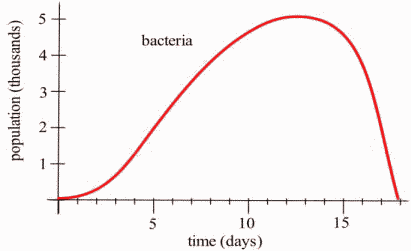
\includegraphics[width=3.00000in,height=2.00000in]{media/image114.wmf}

\begin{quote}
Figure 9

a. Is this an exponential function with base \emph{b} \textgreater{} 1,
an exponential function with\\
0 \textless{} \emph{b} \textless{} 1, or a logarithmic function with
base \emph{b} \textgreater{} 1?

b. What is the value of \emph{b} (the base) for this graph? How do you
know?
\end{quote}

\begin{enumerate}
\item ~
  \hypertarget{chapter-2-the-derivative}{\section{Chapter 2: The
  Derivative}\label{chapter-2-the-derivative}}

  \hypertarget{precalculus-idea-slope-and-rate-of-change}{\subsection{Precalculus
  Idea: Slope and Rate of
  Change}\label{precalculus-idea-slope-and-rate-of-change}}
\end{enumerate}

The slope of a line measures how fast a line rises or falls as we move
from left to right along the line. It measures the rate of change of the
y-coordinate with respect to changes in the x-coordinate. If the line
represents the distance traveled over time, for example, then its slope
represents the velocity. In Figure 1, you can remind yourself of how we
calculate slope using two points on the line:

\textbf{m = \{ slope from P to Q \} = = = }

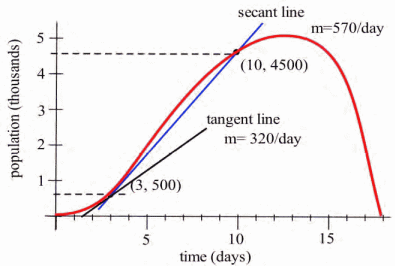
\includegraphics[width=2.73611in,height=1.99028in]{media/image115.emf}

\begin{quote}
Figure 10
\end{quote}

We would like to be able to get that same sort of information (how fast
the curve rises or falls, velocity from distance) even if the graph is
not a straight line. But what happens if we try to find the slope of a
curve, as in Figure 2? We need two points in order to determine the
slope of a line. How can we find a slope of a curve, at just one point?

\begin{quote}
\includegraphics[width=1.88403in,height=1.27917in]{media/image3.png}
\end{quote}

Figure 11

The answer, as suggested in Figure 2 is to find the slope of the tangent
line to the curve at that point. Most of us have an intuitive idea of
what a tangent line is. Unfortunately, ``tangent line'' is hard to
define precisely.

\textbf{Definition:} A \textbf{secant line} is a line between two points
on a curve.

\textbf{Can't-quite-do-it-yet Definition:} A \textbf{tangent line} is a
line at one point on a curve \ldots{}. that does its best to be the
curve at that point?

It turns out that the easiest way to define the tangent line is to
define its slope.

\begin{enumerate}
\item ~
  \hypertarget{section-1-instantaneous-rate-of-change-and-tangent-lines}{\subsection{Section
  1: Instantaneous Rate of Change and Tangent
  Lines}\label{section-1-instantaneous-rate-of-change-and-tangent-lines}}

  \begin{enumerate}
  \item ~
    \subsubsection{Instantaneous Velocity}\label{instantaneous-velocity}
  \end{enumerate}
\end{enumerate}

Suppose we drop a tomato from the top of a 100 foot building and time
its fall .
\includegraphics[width=4.32083in,height=2.19792in]{media/image116.emf}

\begin{quote}
Figure 12
\end{quote}

Some questions are easy to answer directly from the table:

\begin{quote}
(a) How long did it take for the tomato n to drop 100 feet? (2.5
seconds)

(b) How far did the tomato fall during the first second? (100 -- 84 = 16
feet)

(c) How far did the tomato fall during the last second? (64 -- 0 = 64
feet)

(d) How far did the tomato fall between t =.5 and t = 1? (96 -- 84 = 12
feet)
\end{quote}

Some other questions require a little calculation:

\begin{quote}
(e) What was the average velocity of the tomato during its fall?

\textbf{Average velocity = =} = = --40 ft/s .

(f) What was the average velocity between t=1 and t=2 seconds?

Average velocity = = = = --48 ft/s .
\end{quote}

Some questions are more difficult.

\begin{quote}
(g) How fast was the tomato falling 1 second after it was dropped?

This question is significantly different from the previous two questions
about average velocity. Here we want the \textbf{instantaneous
velocity,} the velocity at an instant in time. Unfortunately the tomato
is not equipped with a speedometer so we will have to give an
approximate answer.

One crude approximation of the instantaneous velocity after 1 second is
simply the average velocity during the entire fall, --40 ft/s . But the
tomato fell slowly at the beginning and rapidly near the end so the
"--40 ft/s" estimate may or may not be a good answer.

We can get a better approximation of the instantaneous velocity at t=1
by calculating the average velocities over a short time interval near t
= 1 . The average velocity between t = 0.5 and t = 1 is ~=~--24 ft/s,
and the average velocity between t = 1 and t = 1.5 is = --40 ft/s so we
can be reasonably sure that the instantaneous velocity is between --24
ft/s and --40 ft/s.
\end{quote}

In general, the shorter the time interval over which we calculate the
average velocity, the better the average velocity will approximate the
instantaneous velocity. The average velocity over a time interval is ,
which is the slope of the \textbf{secant line} through two points on the
graph of height versus time (Fig. 4). The instantaneous velocity at a
particular time and height is the slope of the \textbf{tangent line} to
the graph at the point given by that time and height.

\includegraphics[width=3.02847in,height=2.66042in]{media/image117.emf}

\begin{quote}
Figure 13

\textbf{Average velocity = = slope of the secant line through 2 points.}

\textbf{Instantaneous velocity = slope of the line tangent to the
graph.}
\end{quote}

\subsubsection{Tangent Lines}\label{tangent-lines}

Do this!

The graph below is the graph of . We want to find the slope of the
tangent line at the point (1, 2).

First, draw the secant line between (1, 2) and (2, −1) and compute its
slope.

Now draw the secant line between (1, 2) and (1.5, 1) and compute its
slope.

Compare the two lines you have drawn. Which would be a better
approximation of the tangent line to the curve at

(1, 2)?

Now draw the secant line between (1, 2) and (1.3, 1.5) and compute its
slope. Is this line an even better approximation of the tangent line?

Now draw your best guess for the tangent line and measure its slope. Do
you see a pattern in the slopes?

\includegraphics[width=5.32292in,height=2.41667in]{media/image119.png}

\begin{quote}
Figure 14
\end{quote}

You should have noticed that as the interval got smaller and smaller,
the secant line got closer to the tangent line and its slope got closer
to the slope of the tangent line. That's good news -- we know how to
find the slope of a secant line.

\textbf{Example:} Now let's look at the problem of finding the slope of
the line L (Figure 6) which is tangent to f(x) = x2 at the point (2,4).

We could estimate the slope of L from the graph, but we won't. Instead,
we will use the idea that secant lines over tiny intervals approximate
the tangent line.

\includegraphics[width=2.82083in,height=2.82083in]{media/image120.emf}\includegraphics[width=2.28333in,height=2.63194in]{media/image121.emf}

\begin{quote}
Figure 15 Figure 16
\end{quote}

We can see that the line through (2,4) and (3,9) on the graph of f is an
approximation of the slope of the tangent line, and we can calculate
that slope exactly: m = ∆y/∆x = (9--4)/(3--2) = 5. But m = 5 is only an
estimate of the slope of the tangent line and not a very good estimate.
It's too big. We can get a better estimate by picking a second point on
the graph of f which is closer to (2,4) ---- the point (2,4) is fixed
and it must be one of the points we use. From Figure 7, we can see that
the slope of the line through the points (2,4) and (2.5,6.25) is a
better approximation of the slope of the tangent line at (2,4): m =
∆y/∆x = (6.25 -- 4)/(2.5 -- 2) = 2.25/.5 = 4.5 , a better estimate, but
still

an approximation. We can continue picking points closer and closer to
(2,4) on the graph of f, and then calculating the slopes of the lines
through each of these points and the point (2,4):

\begin{quote}
Points to the left of (2,4) Points to the right of (2,4)

x y = x2 slope of line through x y = x2 slope of line through

\emph{(x,y) and (2,4)} \emph{(x,y) and (2,4)}

1.5 2.25 3.5 3 9 5

1.9 3.61 3.9 2.5 6.25 4.5

1.99 3.9601 3.99 2.01 4.0401 4.01
\end{quote}

The only thing special about the x--values we picked is that they are
numbers which are close, and very close, to

x = 2. Someone else might have picked other nearby values for x. As the
points we pick get closer and closer to

the point (2,4) on the graph of y = x2 , the slopes of the lines through
the points and (2,4) are better approximations of the slope of the
tangent line, and these slopes are getting closer and closer to 4.

We can bypass much of the calculating by not picking the points one at a
time: let's look at a general point near (2,4). Define x = 2 + h so h is
the increment from 2 to x (Fig. 8). If h is small, then x = 2 + h is
close to 2 and the point (2+h, f(2+h) ) = (2+h, (2+h)2 ) is close to
(2,4). The slope m of the line through the points (2,4) and (2+h, (2+h)2
) is a good approximation of the slope of the tangent line at the point
(2,4):

\includegraphics[width=2.86806in,height=2.36806in]{media/image122.emf}

\begin{quote}
Figure 17
\end{quote}

m = = = = = = 4 + h .

If h is very small, then m = 4 + h is a very good approximation to the
slope of the tangent line, and m = 4 + h is very close to the value 4.

The value m~=~4 + h is the slope of the secant line through the two
points (2,4) and ( 2+h, (2+h)2 ). As h gets smaller and smaller, this
slope approaches the slope of the tangent line to the graph of f at
(2,4).

In some applications, we need to know where the graph of a function f(x)
has horizontal tangent lines (slopes = 0). In Fig. 3, the slopes of the
tangent lines to graph of y = f(x) are 0 when x = 2 or x ≈ 4.5 .

\textbf{Example:} At right is the graph of y = g(x). At what values of x
does the graph of y = g(x) in Fig. 9 have horizontal tangent lines?

\includegraphics[width=2.73611in,height=1.08472in]{media/image123.emf}

\begin{quote}
Figure 18
\end{quote}

\textbf{Solution:} The tangent lines to the graph of g are horizontal
(slope = 0) when x ≈ --1, 1, 2.5, and 5.

\begin{enumerate}
\item ~
  \hypertarget{section-2-the-derivative}{\subsection{Section 2: The
  Derivative}\label{section-2-the-derivative}}

  \begin{enumerate}
  \item ~
    \subsubsection{Definition of the
    Derivative}\label{definition-of-the-derivative}
  \end{enumerate}
\end{enumerate}

The tangent line problem and the instantaneous velocity problem are the
same problem. In each problem we wanted to know how rapidly something
was \textbf{changing at an instant in time}, and the answer turned out
to be finding the \textbf{slope of a tangent line,} which we
approximated with the \textbf{slope of a secant line}. This idea is the
key to defining the slope of a curve.

\textbf{The Derivative:}

The \textbf{derivative} of a function f at a point (x, f(x)) is the
instantaneous rate of change.

The \textbf{derivative} is the slope of the tangent line to the graph of
f at the point (x, f(x)).

The \textbf{derivative} is the slope of the curve f(x) at the point (x,
f(x)).

A function is called \textbf{differentiable} at (x, f(x)) if its
derivative exists at (x, f(x)).

\textbf{Notation for the Derivative:}

The \textbf{derivative of y = f(x) with respect to x} is written as

(read aloud as ``f prime of x''), or (``y prime'')

or (read aloud as ``dee why dee ex''), or

The notation that resembles a fraction is called \textbf{Leibniz
notation}. It displays not only the name of the function (f or y), but
also the name of the variable (in this case, x). It looks like a
fraction because the derivative is a slope. In fact, this is simply
written in Roman letters instead of Greek letters.

\textbf{Verb forms:}

We \textbf{find the derivative} of a function, or \textbf{take the
derivative} of a function, or \textbf{differentiate} a function.

We use an adaptation of the notation to mean ``find the derivative of
f(x):''

\textbf{Formal Algebraic Definition:}

(*)

\textbf{Practical Definition:}

The derivative can be approximated by looking at an average rate of
change, or the slope of a secant line,\\
over a very tiny interval. The tinier the interval, the closer this is
to the true instantaneous rate of change, slope of the tangent line, or
slope of the curve.

\textbf{Looking Ahead:}

We will have methods for computing exact values of derivatives from
formulas soon. If the function is\\
given to you as a table or graph, you will still need to approximate
this way.

(* information about ``lim'' is in Chapter 5: Optional Topics)

This is the foundation for the rest of this chapter. It's remarkable
that such a simple idea (the slope of a tangent line) and such a simple
definition (for the derivative f ' ) will lead to so many important
ideas and applications.

\subsubsection{The Derivative as a
Function}\label{the-derivative-as-a-function}

We now know how to find (or at least approximate) the derivative of a
function for any x-value; this means we can think of the derivative as a
function, too. The inputs are the same x's; the output is the value of
the derivative at

\textbf{Example:} Fig. 10 is the graph of a function. We can use the
information in the graph to fill in a table showing values of:

\begin{quote}
\includegraphics[width=2.54725in,height=1.66279in]{media/image133.png}

Figure 19
\end{quote}

At various values of \emph{x}, draw your best guess at the tangent line
and measure its slope. You might have to extend your lines so you can
read some points. In general, your estimate of the slope will be better
if you choose points that are easy to read and far away from each other.
Here are my estimates for a few values of \emph{x} (parts of the tangent
lines I used are shown):

\begin{longtable}[]{@{}lll@{}}
\toprule
\begin{minipage}[b]{0.32\columnwidth}\raggedright\strut
\strut
\end{minipage} & \begin{minipage}[b]{0.32\columnwidth}\raggedright\strut
\strut
\end{minipage} & \begin{minipage}[b]{0.32\columnwidth}\raggedright\strut
= the estimated SLOPE

of the tangent line to the curve

at the point .\strut
\end{minipage}\tabularnewline
\midrule
\endhead
0 & 0 & 1\tabularnewline
1 & 1 & 0\tabularnewline
2 & 0 & −1\tabularnewline
3 & −1 & 0\tabularnewline
4 & 1 & 1\tabularnewline
5 & 2 & 0.5\tabularnewline
\bottomrule
\end{longtable}

We can estimate the values of f'(x) at some non-integer values of x,
too: f'(.5) ≈ 0.5 and f'(1.3) ≈ --0.3.

We can even think about entire intervals. For example, if 0 \textless{}
x \textless{} 1, then f(x) is increasing, all the slopes are positive,
and so f'(x) is positive.

The values of f'(x) definitely depend on the values of x , and f'(x) is
a function of x. We can use the results in the table to help sketch the
graph of f'(x) in Fig. 11.

\includegraphics[width=2.76042in,height=1.93750in]{media/image138.png}

\begin{quote}
Figure 20
\end{quote}

\textbf{Example:} Fig. 12 is the graph of the height h(t) of a rocket at
time t. Sketch the graph of the \textbf{velocity} of the rocket at time
t. (Velocity is the \textbf{derivative} of the height function, so it is
the \textbf{slope of the tangent} to the graph of position or height.)

\begin{quote}
\includegraphics[width=2.44306in,height=1.66042in]{media/image139.emf}

Figure 21
\end{quote}

\textbf{Solution:} The lower graph in Fig. 13 shows the velocity of the
rocket. This is v(t) = h'(t).

\begin{quote}
\includegraphics[width=2.73958in,height=3.39583in]{media/image140.png}

Figure 22
\end{quote}

\hypertarget{section-3-rates-in-real-life}{\subsection{Section 3: Rates
in Real Life}\label{section-3-rates-in-real-life}}

So far we have emphasized the derivative as the slope of the line
tangent to a graph . That interpretation is very visual and useful when
examining the graph of a function, and we will continue to use it.
Derivatives, however, are used in a wide variety of fields and
applications, and some of these fields use other interpretations. The
following are a few interpretations of the derivative that are commonly
used.

\textbf{\emph{General}}

\begin{quote}
Rate of Change: f '(x) is the \textbf{rate of change} of the function at
x. If the units for x are years and the units for f(x) are people, then
the units for are , a rate of change in population.
\end{quote}

\textbf{\emph{Graphical}}

\begin{quote}
Slope: f '(x) is the \textbf{slope of the line tangent to the graph of f
at the point ( x, f(x) ).}
\end{quote}

\textbf{\emph{Physical}}

\begin{quote}
Velocity: If f(x) is the position of an object at time x, then f '(x) is
the \textbf{velocity} of the object at time x. If

the units for x are hours and f(x) is distance measured in miles, then
the units for \textbf{f '}(x)~=~~~are~~,

miles per hour, which is a measure of velocity.

Acceleration If f(x) is the velocity of an object at time x, then f '(x)
is the \textbf{acceleration} of the object at time

x. If the units are for x are hours and f(x) has the units ~, then the
units for the acceleration \textbf{f '(x)} =

are = , miles per hour per hour.
\end{quote}

\textbf{\emph{Business}}

\begin{quote}
Marginal Cost If f(x) is the total cost of x objects, then \textbf{f
'(}x\textbf{)} is the \textbf{marginal cost}, at a production level

of x. This marginal cost is approximately the \emph{additional} cost of
making one more object once we have

already made x objects. If the units for x are bicycles and the units
for f(x) are dollars, then the units for

f '(x) = are~~, the cost per bicycle.

Marginal Profit If f(x) is the total profit from producing and selling x
objects, then \textbf{f~'(}x\textbf{)} is the \textbf{marginal }

\textbf{profit}, the profit to be made from producing and selling one
more object. If the units for x are bicycles and

the units for f(x) are dollars, then the units for f~'(x)~=~~~~ are~~,
dollars per bicycle, which is the

profit per bicycle.

In business contexts, the word "marginal" usually means the derivative
or rate of change of some quantity.
\end{quote}

One of the strengths of calculus is that it provides a unity and economy
of ideas among diverse applications. The vocabulary and problems may be
different, but the ideas and even the notations of calculus are still
useful.

\subsubsection{Business and Economics
Terms}\label{business-and-economics-terms}

Suppose you are producing and selling some item. The profit you make is
the amount of money you take in minus what you have to pay to produce
the items. Both of these quantities depend on how many you make and
sell. (So we have functions here.) Here is a list of definitions for
some of the terminology, together with their meaning in algebraic terms
and in graphical terms.

Your \textbf{cost} is the money you have to spend to produce your items.

The \textbf{Fixed Cost (FC)} is the amount of money you have to spend
regardless of how many items you produce. FC can include things like
rent, purchase costs of machinery, and salaries for office staff. You
have to pay the fixed costs even if you don't produce anything.

The \textbf{Total Variable Cost (TVC)} for q items is the amount of
money you spend to actually produce them. TVC includes things like the
materials you use, the electricity to run the machinery, gasoline for
your delivery vans, maybe the wages of your production workers. These
costs will vary according to how many items you produce.

The \textbf{Total Cost (TC)} for q items is the total cost of producing
them. It's the sum of the fixed cost and the total variable cost for
producing q items.

The \textbf{Average Cost (AC)} for q items is the total cost divided by
q, or TC/q. You can also talk about the average fixed cost, FC/q, or the
average variable cost, TVC/q.

\textbf{Demand} is the functional relationship between the price
\textbf{p} and the quantity \textbf{q} that can be sold (that is
demanded). Depending on your situation, you might think of \textbf{p} as
a function of \textbf{q}, or of \textbf{q} as a function of \textbf{p}.

Your \textbf{revenue} is the amount of money you actually take in from
selling your products. Revenue is price × quantity.

The \textbf{Total Revenue (TR)} for q items is the total amount of money
you take in for selling q items.

The \textbf{Average Revenue (AR)} for q items is the total revenue
divided by q, or TR/q.

The \textbf{Profit (π)} for q items is TR(q) -- TC(q).

The average profit for q items is \textbf{π}/q. The marginal profit at q
items is π(q + 1) -- π(q), or

\begin{quote}
\textbf{Example:} Why is it OK that are there two definitions for
Marginal Cost (and Marginal Revenue, and Marginal Profit)?

We have been using slopes of secant lines over tiny intervals to
approximate derivatives. In this example, we'll turn that around --
we'll use the derivative to approximate the slope of the secant line.

Notice that the ``cost of the next item'' definition is actually the
slope of a secant line, over an interval of 1 unit:

So this is approximately the same as the derivative of the cost function
at \emph{q}:

In practice, these two numbers are so close that there's no practical
reason to make a distinction. For our purposes, the marginal cost
\textbf{is} the derivative \textbf{is} the cost of the next item.
\end{quote}

\textbf{Graphical Interpretations of the Basic Business Math Terms}

\textbf{Illustration/Example:}

Here are the graphs of TR and TC for producing and selling a certain
item. The horizontal axis is the number of items, in thousands. The
vertical axis is the number of dollars, also in thousands.

\includegraphics[width=5.04651in,height=2.63525in]{media/image144.png}

\begin{quote}
Figure 23
\end{quote}

First, notice how to find the fixed cost and variable cost from the
graph here. \textbf{FC is the y-intercept of the TC graph.} (FC =
TC(0).) The graph of TVC would have the same shape as the graph of TC,
shifted down. (TVC = TC -- FC.)

We already know that we can find average rates of change by finding
slopes of secant lines. AC, AR, MC, and MR are all rates of change, and
we can find them with slopes, too.

\textbf{AC(q) is the slope of a diagonal line, from (0, 0) to (q,
TC(q)).} \textbf{AR(q) is the slope of the line from (0, 0) to (q,
TR(q)).}

MC(q) = TC(q + 1) -- TC(q), but that's impossible to read on this graph.
How could you distinguish between TC(4022) and TC(4023)? On this graph,
that interval is too small to see, and our best guess at the secant line
is actually the tangent line to the TC curve at that point. (This is the
reason we want to have the derivative definition handy.)

\textbf{MC(q) is the slope of the tangent line to the TC curve at (q,
TC(q)). In a similar way, MR(q) is the slope of the tangent line to the
TR curve at (q, TR(q)).}

\textbf{Profit is the distance between the TR and TC curve.} If you
experiment with your clear plastic ruler, you'll see that the biggest
profit occurs exactly when the tangent lines to the TR and TC curves are
parallel. This is the rule \textbf{``profit is maximized when MR =
MC.''}

\subsubsection{Rates in Real Life}\label{rates-in-real-life}

\textbf{Example:} You can estimate a tree's age in years by multiplying
its diameter (measured in inches) by its growth factor (a number that
depends on the species). According to the Missouri Department of
Conservation, the Growth factor for a cottonwood tree is 2.

\begin{enumerate}
\def\labelenumi{\alph{enumi}.}
\item
  Suppose you find a cottonwood tree in Missouri that is 6 inches in
  diameter. How old would you estimate it to be?
\item
  What are the units of the growth factor?
\item
  Is this growth factor a derivative?
\end{enumerate}

\textbf{Solution:} a. The cottonwood tree should be about 6 × 2 = 12
years old.

\begin{quote}
b. The units of the growth factor are years per inch (because when we
multiply the growth factor by inches, we get years).

c. Yes, the growth factor is a derivative. It has fractional units
(years per inch), so it represents a rate. In this case, it's the
derivative of the function that gives the age of a tree as a function of
its diameter. The function is linear, so the derivative in this case is
the constant slope, 2 years per inch.
\end{quote}

\textbf{Example:} The length of day (that is, daylight) in Seattle is a
function of the day of the year. For example, on August
12\textsuperscript{th}, 2012, there were about 14 hours 24 minutes of
daylight. In Seattle, August is the summer, approaching the autumnal
equinox. The days are decreasing in length by about three minutes per
day. So the derivative of this function is about −3 minutes per day. On
January 15, 2012, which is wintertime in Seattle, there were about 8
hours 52 minutes of daylight, and the derivative was about (positive) 2
minutes per day; the length of the day was increasing by about 2 minutes
a day.

\hypertarget{section-4-derivatives-of-formulas}{\subsection{Section 4:
Derivatives of Formulas}\label{section-4-derivatives-of-formulas}}

In this section, we'll get the derivative rules that will let us find
formulas for derivatives when our function comes to us as a formula.
This is a very algebraic section, and you should get lots of practice.
When you tell someone you have studied calculus, this is the one skill
they will expect you to have. There's not a lot of deep meaning here --
these are strictly algebraic rules.

\subsubsection{Building Blocks}\label{building-blocks}

These are the simplest rules -- rules for the basic functions. We won't
prove these rules; we'll just use them. But first, let's look at a few
so that we can see they make sense.

\begin{quote}
\textbf{Example:} Find the derivative of

\textbf{Solution:} This is a linear function, so its graph is its own
tangent line! The slope of the tangent line, the derivative, is the
slope of the line:

\textbf{Rule: The derivative of a linear function is its slope}

\textbf{Example:} Find the derivative of

\textbf{Solution:} Think about this one graphically, too. The graph of
\emph{f}(\emph{x}) is a horizontal line. So its slope is zero.

\textbf{Rule: The derivative of a constant is zero}

\textbf{Example:} I will just tell you that the derivative of is . Now
think about the function . What will its derivative be?

\textbf{Solution:} Think about what this change means to the graph of
\emph{g} -- it's now 4 times as tall as the graph of \emph{f}. If we
find the slope of a secant line, it will be ; each slope will be 4 times
the slope of the secant line on the \emph{f} graph. This property will
hold for the slopes of tangent lines, too:

\textbf{Rule: Constants come along for the ride.}
\end{quote}

OK, enough of that. Here are the basic rules, all in one place.

\textbf{Derivative Rules: Building Blocks}

In what follows, \emph{f} and \emph{g} are differentiable functions of
\emph{x}.

(a) \textbf{Constant Multiple Rule:}

(b) \textbf{Sum (or Difference) Rule: (or )}

(c) \textbf{Power Rule: }

Special cases: (because )

(because )

(d) \textbf{Exponential Functions: }

(e) \textbf{Natural Logarithm:}

The sum, difference, and constant multiple rule combined with the power
rule allow us to easily find the derivative of any polynomial.

\begin{quote}
\textbf{Example:} Find the derivative of

\textbf{Solution: }
\end{quote}

No, you don't have to show every single step. Do be careful when you're
first working with the rules, but pretty soon you'll be able to just
write down the derivative directly:

\begin{quote}
\textbf{Example:}
\end{quote}

The power rule works even if the power is negative or a fraction. In
order to apply it, first translate all roots and one-overs into
exponents:

\begin{quote}
\textbf{Example:} Find the derivative of

\textbf{Solution:} First step -- translate into exponents:

Now you can take the derivative:

Be careful when finding the derivatives with negative exponents.

\textbf{Example :} The cost to produce x items is hundred dollars.

(a) What is the cost for 100 items? 101 items? What is cost of the
101\textsuperscript{st} item?

(b) For f(x) = , calculate f '(x) and evaluate f ' at x = 100. How does
f '(100) compare with the last answer in part (a)?

\textbf{Solution:}

(a) Put f(x) = = x1/2 hundred dollars, the cost for x items. Then f(100)
= \$1000 and f(101) = \$1004.99, so it costs \$4.99 for that
101\textsuperscript{st} item. Using this definition, the marginal cost
is \$4.99.

(b) f '(x) = x--1/2 = so f '(100) = = hundred dollars = \$5.00. Note how
close these answers are! This shows (again) why it's OK that we use both
definitions for marginal cost.
\end{quote}

\subsubsection{Product and Quotient
Rules}\label{product-and-quotient-rules}

The basic rules will let us tackle simple functions. But what happens if
we need the derivative of a combination of these functions?

\begin{quote}
\textbf{Example:} Find the derivative of

\textbf{Solution:} This function is not a simple sum or difference of
polynomials. It's a product of polynomials. We can simply multiply it
out to find its derivative:
\end{quote}

\textbf{\\
}

\begin{quote}
\textbf{Example:} Find the derivative of

\textbf{Solution:} This function is not a simple sum or difference of
polynomials. It's a product of polynomials. We \textbf{could} simply
multiply it out to find its derivative as before -- who wants to
volunteer? Nobody?
\end{quote}

We'll need a rule for finding the derivative of a product so we don't
have to multiply everything out.

Is the rule what we hope it is, that we can just take the derivatives of
the factors and multiply them? Unfortunately, no -- that won't give the
right answer.

\begin{quote}
\textbf{Example:} Find the derivative of

\textbf{Solution:} We already worked out the derivative. It's . What if
we try differentiating the factors and multiplying them? We'd get ,
which is totally different from the correct answer.
\end{quote}

The rules for finding derivatives of products and quotients are a little
complicated, but they save us the much more complicated algebra we might
face if we were to try to multiply things out. They also let us deal
with products where the factors are not polynomials. We can use these
rules, together with the basic rules, to find derivatives of many
complicated looking functions.

\textbf{Derivative Rules: Product and Quotient Rules}

In what follows, \emph{f} and \emph{g} are differentiable functions of
\emph{x}.

(f) \textbf{Product Rule:}

The derivative of the first factor times the second left alone, plus the
first left alone times the derivative of the second.

The product rule can extend to a product of several functions; the
pattern continues -- take the derivative of each factor in turn,
multiplied by all the other factors left alone, and add them up.

(g) \textbf{Quotient Rule:}

The numerator of the result resembles the product rule, but there is a
minus instead of a plus; the minus sign goes with the g'. The
denominator is simply the square of the original denominator -- no
derivatives there.

\begin{quote}
\textbf{Example:} Find the derivative of

\textbf{Solution:} This is a product, so we need to use the product
rule. I like to put down empty parentheses to remind myself of the
pattern; that way I don't forget anything.

Then I fill in the parentheses -- the first set gets the derivative of ,
the second gets left alone, the third gets left alone, and the fourth
gets the derivative of .
\end{quote}

Notice that this was one we couldn't have done by ``multiplying out.''

\textbf{\\
}

\begin{quote}
\textbf{Example:} Find the derivative of

\textbf{Solution:} This is a quotient, so we need to use the quotient
rule. Again, I find it helpful to put down the empty parentheses as a
template:

Then I fill in all the pieces:

Now for goodness' sakes don't try to simplify that! Remember that
``simple'' depends on what you will do next; in this case, we were asked
to find the derivative, and we've done that. Please STOP!
\end{quote}

\subsubsection{Chain Rule}\label{chain-rule}

There is one more type of complicated function that we will want to know
how to differentiate: composition. The Chain Rule will let us find the
derivative of a composition. (This is the last derivative rule we will
learn!)

\begin{quote}
\textbf{Example:} Find the derivative of .

\textbf{Solution:} This is not a simple polynomial, so we can't use the
basic building block rules yet. It is a product, so we could write it as
and use the product rule. Or we could multiply it out and simply
differentiate the resulting polynomial. I'll do it the second way:
\end{quote}

\textbf{\\
}

\begin{quote}
\textbf{Example:} Find the derivative of

\textbf{Solution:} We \textbf{could} write it as a product with 20
factors and use the product rule, or we \textbf{could} multiply it out.
But I don't want to do that, do you?
\end{quote}

We need an easier way, a rule that will handle a composition like this.
The Chain Rule is a little complicated, but it saves us the much more
complicated algebra of multiplying something like this out. It will also
handle compositions where it wouldn't be possible to ``multiply it
out.''

The Chain Rule is the most common place for students to make mistakes.
Part of the reason is that the notation takes a little getting used to.
And part of the reason is that students often forget to use it when they
should. When should you use the Chain Rule? Almost every time you take a
derivative.

\textbf{Derivative Rules: Chain Rule}

In what follows, \emph{f} and \emph{g} are differentiable functions with
and

(h) \textbf{Chain Rule (Leibniz notation):}

Notice that the du's seem to cancel. This is one advantage of the
Leibniz notation; it can remind you of how the chain rule chains
together.

(h) \textbf{Chain Rule (using prime notation):}

(h) \textbf{Chain Rule (in words): }

The derivative of a composition is) the derivative of the outside TIMES
the derivative of what's inside.

I recite the version in words each time I take a derivative, especially
if the function is complicated.

\begin{quote}
\textbf{Example:} Find the derivative of .

\textbf{Solution:} This is the same one we did before by multiplying
out. This time, let's use the Chain Rule: The inside function is what
appears inside the parentheses: . The outside function is the first
thing we find as we come in from the outside -- it's the square
function, something\textsuperscript{2}. We want the derivative of the
outside\\
(2 something) TIMES the derivative of what's inside (which is ):

(By the way, if you multiply this out, you get the same answer we got
before. Hurray! Algebra works!)

\textbf{Example:} Find the derivative of

\textbf{Solution:} Now we have a way to handle this one. It's the
derivative of the outside TIMES the derivative of what's inside.

\textbf{Example :} Differentiate .

\textbf{Solution:} This isn't a simple exponential function; it's a
composition. Typical calculator or computer syntax can help you see what
the ``inside'' function is here. On a TI calculator, for example, when
you push the key, it opens up parentheses: This tells you that the
``inside'' of the exponential function is the exponent. Here, the inside
is the exponent. Now we can use the Chain Rule: We want the derivative
of the outside TIMES the derivative of what's inside. The outside is the
``e to the'' function, so its derivative is the same thing. The
derivative of what's inside is 2x. So
\end{quote}

\textbf{Example:} The table gives values for f , f ' , g and g ' at a
number of points. Use these values to

determine ( f°g )(x) and \textbf{(} f°g \textbf{) '}(x) at x = --1 and
0.

\begin{quote}
x f(x) g(x) f '(x) g '(x) ( f°g )(x) \textbf{(} f°g \textbf{) '}(x)

~~\emph{~~~~~~~~~~~~~~~~~~~~~~~~~~~~~~~~~~~~~~~~~~~~~~~~~~~~~~~~~~~~~~~~~
~ ~}

--1 2 3 1 0

0 --1 1 3 2

1 1 0 --1 3

2 3 --1 0 1

3 0 2 2 --1
\end{quote}

\textbf{Solution:} ( f°g )(--1) = f( g(--1) ) = f( 3 ) = 0 and ( f°g
)(0) = f( g(0) ) = f( 1 ) = 1.

\begin{quote}
\textbf{(} f°g \textbf{) '}(--1) = \textbf{f '(} g(--1) \textbf{).g '(}
--1 \textbf{)} = \textbf{f '(} 3 \textbf{).}(0) = (2)(0) = 0 and

\textbf{(} f°g \textbf{) '}( 0 ) = \textbf{f '(} g( 0 ) \textbf{).g '(}
0 \textbf{)} = \textbf{f '(} 1 \textbf{).}( 2 ) = (--1)(2) = --2 .

I'll let you do the rest.
\end{quote}

\subsubsection{Derivatives of Complicated
Functions}\label{derivatives-of-complicated-functions}

You're now ready to take the derivative of some mighty complicated
functions. But how do you tell what rule applies first? Come in from the
outside -- what do you encounter first? That's the first rule you need.
Use the Product, Quotient, and Chain Rules to peel off the layers, one
at a time, until you're all the way inside.

\textbf{\\
}

\begin{quote}
\textbf{Example:} Find

\textbf{Solution:} Coming in from the outside, I see that this is a
product of two (complicated) functions. So I'll need the Product Rule
first. I'll fill in the pieces I know, and then I can figure the rest as
separate steps and substitute in at the end:

Now as separate steps, I'll find

(using the Chain Rule) and

(also using the Chain Rule).

Finally, to substitute these in their places:

(And please don't try to simplify that!)

\textbf{Example:} Differentiate

\textbf{Solution:} Don't panic! As you come in from the outside, what's
the first thing you encounter? It's that 4\textsuperscript{th} power.
That tells you that this is a composition, a (complicated) function
raised to the 4\textsuperscript{th} power.

\textbf{Step One:} Use the Chain Rule. The derivative of the outside
TIMES the derivative of what's inside.

Now we're one step inside, and we can concentrate on just the part. Now,
as you come in from the outside, the first thing you encounter is a
quotient -- this is the quotient of two (complicated) functions.

\textbf{Step Two:} Use the Quotient Rule:

Now we've gone one more step inside, and we can concentrate on just the
part. Now we have a product.

\textbf{Step Three:} Use the Product Rule:

And now we're all the way in -- no more derivatives to take.

\textbf{Step Four:} Now it's just a question of substituting back -- be
careful now!

, so

, so

.

\textbf{Phew!}
\end{quote}

\subsubsection{What if the Derivative Doesn't
Exist?}\label{what-if-the-derivative-doesnt-exist}

A function is called \textbf{differentiable} at a point if its
derivative exists at that point.

We've been acting as if derivatives exist everywhere for every function.
This is true for most of the functions that you will run into in this
class. But there are some common places where the derivative doesn't
exist.

Remember that the derivative is the slope of the tangent line to the
curve. That's what to think about.

\textbf{Where can a slope not exist?} If the tangent line is vertical,
the derivative will not exist.

\begin{quote}
\textbf{Example:} This is the graph of f(x) = = x1/3 . Notice that the
tangent line to this curve at \emph{x} = 0 is vertical. So its slope
does not exist, and so the derivative does not exist at \emph{x} = 0.

\includegraphics[width=3.94792in,height=2.04167in]{media/image220.png}

Figure 24
\end{quote}

\textbf{Where can a tangent line not exist?} If there is a corner in the
graph, the derivative will not exist at that point because there is no
well-defined tangent line (a teetering tangent, if you will.) Or if
there is a jump in the graph, the tangent line will be different on
either side and the derivative can't exist.

\begin{quote}
\textbf{Example:} This is the graph of the Greatest Integer Function, a
basic step function. There is no single

tangent line at \emph{x} = 1; the tangent lines on either side are
different. So the derivative does not exist at \emph{x} = 1.

\includegraphics[width=2.50000in,height=1.85417in]{media/image221.png}

Figure 25
\end{quote}

\begin{enumerate}
\item ~
  \hypertarget{section-5-second-derivative-and-concavity}{\subsection{Section
  5: Second Derivative and
  Concavity}\label{section-5-second-derivative-and-concavity}}

  \begin{enumerate}
  \item ~
    \subsubsection{Second Derivative and
    Concavity}\label{second-derivative-and-concavity}
  \end{enumerate}
\end{enumerate}

Graphically, a function is \textbf{concave up} if its graph is curved
with the opening upward (Fig. 17a). Similarly, a function is
\textbf{concave down} if its graph opens downward (Fig. 17b).

\begin{quote}
\includegraphics[width=2.78333in,height=1.21667in]{media/image222.emf}

Figure 26
\end{quote}

For example, \textbf{An Epidemic:} Suppose an epidemic has started, and
you, as a member of congress, must decide whether the current methods
are effectively fighting the spread of the disease or whether more
drastic measures and more money are needed. In Fig. 18, f(x) is the
number of people who have the disease at time x, and two different
situations are shown. In both (a) and (b), the number of people with the
disease, f(now), and the rate at which new people are getting sick, f
'(now), are the same. The difference in the two situations is the
concavity of f, and that difference in concavity might have a big effect
on your decision.

\begin{quote}
\includegraphics[width=3.31250in,height=1.84375in]{media/image223.png}

Figure 27

In (a), f is concave down at "now", the slopes are decreasing, and it
looks as if it's tailing off. We can say ``f is increasing at a
decreasing rate.'' It appears that the current methods are starting to
bring the epidemic under control.

In (b), f is concave up, the slopes are increasing, and it looks as if
it will keep increasing faster and faster. It appears that the epidemic
is still out of control.
\end{quote}

The differences between the graphs come from whether the
\emph{derivative} is increasing or decreasing.

The derivative of a function f is a function that gives information
about the slope of f. \textbf{The derivative tells us if the original
function is increasing or decreasing.}

Because f ` is a function, we can take its derivative. This second
derivative also gives us information about our original function f. The
second derivative gives us a mathematical way to tell how the graph of a
function is curved. \textbf{The second derivative tells us if the
original function is concave up or down.}

\textbf{Second Derivative} Let

The \textbf{second derivative of f} is the derivative of .

Using prime notation, this is or . You can read this aloud as ``y double
prime.''

Using Leibniz notation, the second derivative is written or . This is
read aloud as ``the second derivative of f.

If is positive on an interval, the graph of is \textbf{concave up} on
that interval\textbf{.} We can say that \emph{f} is increasing (or
decreasing) \textbf{at an increasing rate}.

If is negative on an interval, the graph of is \textbf{concave down} on
that interval\textbf{.} We can say that \emph{f} is increasing (or
decreasing) \textbf{at a decreasing rate.}

\begin{quote}
\textbf{Example:} Find for

\textbf{Solution:} First, we need to find the first derivative:

Then we take the derivative of that function:
\end{quote}

If f(x) represents the position of a particle at time x, then v(x) = f
'(x) will represent the velocity (rate of change of the position) of the
particle and a(x) = v '(x) = f ''(x) will represent the acceleration
(the rate of change of the velocity) of the particle.

\textbf{Example :} The height (feet) of a particle at time t seconds is
t3 -- 4t2 + 8t . Find the height,

velocity and acceleration of the particle when t = 0, 1, and 2 seconds.

\textbf{Solution:} f(t) = t3 -- 4t2 + 8t so f(0) = 0 feet, f(1) = 5
feet, and f(2) = 8 feet.

The velocity is v(t) = f '(t) = 3t2 -- 8t + 8 so v(0) = 8 ft/s , v(1) =
3 ft/s, and v(2) = 4 ft/s. At each of these times the velocity is
positive and the particle is moving upward, increasing in height.

The acceleration is a(t) = 6t -- 8 so a(0) = --8 ft/s2 , a(1) = --2
ft/s2 and a(2) = 4 ft/s2 .

\subsubsection{Inflection Points}\label{inflection-points}

\textbf{Definition:} An \textbf{inflection point} is a point on the
graph of a function where the concavity of the

function changes, from concave up to down or from concave down to up.

\textbf{Example:} Which of the labeled points in Fig. 19 are inflection
points?

\includegraphics[width=3.19792in,height=1.22917in]{media/image234.png}

\begin{quote}
Figure 28
\end{quote}

\textbf{Solution:} The concavity changes at points b and g. At points a
and h, the graph is concave up on either side, so the concavity does not
change. At points c and f, the graph is concave down on either side. And
at point e, even though the graph looks strange there, the graph is
concave down on both sides -- the concavity does not change.

Inflection points happen when the concavity changes. Because we know the
connection between the concavity of a function and the sign of its
second derivative, we can use this to find inflection points.

\textbf{Working Definition:} An \textbf{inflection point} is a point on
the graph where the second derivative changes sign.

In order for the second derivative to change signs, it must either be
zero or be undefined. So to find the inflection points of a function we
only need to check the points where f ''(x) is 0 or undefined.

Note that it is not enough for the second derivative to be zero or
undefined. We still need to check that the sign of f'' changes sign. The
functions in the next example illustrate what can happen.

\textbf{Example:} Let f(x) = x3 , g(x) = x4 and h(x) = x1/3 (Fig. 20).
For which of these functions is the point (0,0) an inflection point?

\begin{quote}
\includegraphics[width=3.91667in,height=1.51042in]{media/image235.png}

Figure 29
\end{quote}

\textbf{Solution:} Graphically, it is clear that the concavity of f(x) =
x3 and h(x) = x1/3 changes at (0,0), so (0,0) is an inflection point for
f and h. The function g(x) = x4 is concave up everywhere so (0,0) is not
an inflection point of g.

We can also compute the second derivatives and check the sign change.

\begin{quote}
If f(x) = x3 , then f '(x) = 3x2 and f ''(x) = 6x . The only point at
which f ''(x) = 0 or is undefined
\end{quote}

(f ' is not differentiable) is at x~=~0. If x \textless{} 0, then f
''(x) \textless{} 0 so f is concave down. If x \textgreater{} 0 , then

f ''(x) \textgreater{} 0 so f is concave up. At x = 0 the concavity
changes so the point (0,f(0)) = (0,0) is an inflection point of x3 .

If g(x) = x4 , then g '(x) = 4x3 and g ''(x) = 12x2 . The only point at
which g ''(x) = 0 or is undefined is at x~=~0. If x \textless{} 0, then
g ''(x) \textgreater{} 0 so g is concave up. If x \textgreater{} 0 ,
then g ''(x) \textgreater{} 0 so g is also concave up. At x = 0 the
concavity \textbf{does not change} so the point (0, g(0)) = (0,0) is
\textbf{not an inflection point} of x4 . Keep this example in mind!.

If h(x) = x1/3 , then h '(x) = x--2/3 and h ''(x) = -- x--5/3 . h'' is
not defined if x = 0, but h~''(negative~number) \textgreater{} 0 and h
''(positive number) \textless{} 0 so h changes concavity at (0,0) and
(0,0) is an inflection point of h.

\textbf{Example:} Sketch the graph of a function with f(2) = 3, f '(2) =
1, and an inflection point at (2,3) .

\textbf{Solution:} Two solutions are given in Fig. 21.

\begin{quote}
\includegraphics[width=2.91667in,height=1.37500in]{media/image236.png}

Figure 30
\end{quote}

\hypertarget{section-6-optimization}{\subsection{Section 6:
Optimization}\label{section-6-optimization}}

In theory and applications, we often want to maximize or minimize some
quantity. An engineer may want to maximize the speed of a new computer
or minimize the heat produced by an appliance. A manufacturer may want
to maximize profits and market share or minimize waste. A student may
want to maximize a grade in calculus or minimize the hours of study
needed to earn a particular grade.

Without calculus, we only know how to find the optimum points in a few
specific examples (for example, we know how to find the vertex of a
parabola). But what if we need to optimize an unfamiliar function?

The best way we have without calculus is to examine the graph of the
function, perhaps using technology. But our view depends on the viewing
window we choose -- we might miss something important. In addition,
we'll probably only get an approximation this way. (In some cases, that
will be good enough.)

Calculus provides ways of drastically narrowing the number of points we
need to examine to find the exact locations of maximums and minimums,
while at the same time ensuring that we haven't missed anything
important.

\subsubsection{Local Maxima and Minima}\label{local-maxima-and-minima}

Before we examine how calculus can help us find maximums and minimums,
we need to define the concepts we will develop and use.

\textbf{Definitions:} f has a \textbf{local} \textbf{maximum} at a if
f(a) ≥ f(x) for all x near a

f has a \textbf{local} \textbf{minimum} at a if f(a) \textbf{≤} f(x) for
all x near a

f has a \textbf{local extreme} at a if f(a) is a \textbf{local maximum
or minimum.}

The plurals of these are maxima and minima. We often simply say ``max''
or ``min;'' it saves a lot of syllables.

Some books say ``relative'' instead of ``local.''

The process of finding maxima or minima is called \textbf{optimization.}

A point is a local max (or min) if it is higher (lower) than all the
\textbf{nearby points}. These points come from the shape of the graph.

\textbf{Definitions:} f has a \textbf{global maximum} at a if f(a) ≥
f(x) for all x in the domain of f.

f has a \textbf{global minimum} at a if f(a) \textbf{≤} f(x) for all x
in the domain of f.

f has a \textbf{global extreme} at a if f(a) is a \textbf{global maximum
or minimum.}

Some books say ``absolute'' instead of ``global''

A point is a global max (or min) if it is higher (lower) than every
point on the graph. These points come from the shape of the graph
\textbf{and} the window through which we view the graph.

The local and global extremes of the function in Fig. 22 are labeled.
You should notice that every global extreme is also a local extreme, but
there are local extremes that are not global extremes.

\begin{quote}
\includegraphics[width=3.50000in,height=2.20833in]{media/image237.png}

Figure 31
\end{quote}

If h(x) is the height of the earth above sea level at the location x,
then the global maximum of h is h(summit of Mt. Everest) = 29,028 feet.
The local maximum of h for the United States is h(summit of Mt.
McKinley) = 20,320 feet. The local minimum of h for the United States is
h(Death Valley) = -- 282 feet.

\textbf{Example:} The table shows the annual calculus enrollments at a
large university. Which years had local maximum or minimum calculus
enrollments? What were the global maximum and minimum enrollments in
calculus?

\emph{year 1980 81 82 83 84 85 86 87 88 89 90~~}

enrollment 1257 1324 1378 1336 1389 1450 1523 1582 1567 1545 1571

\textbf{Solution:} There were local maxima in 1982 and 1987; the global
maximum was 1582 students in 1987. There were local minima in 1983 and
1989; the global minimum was 1336 students in 1983. I choose not to
think of 1980 as a local minimum or 1990 as a local maximum. However,
some books would include the endpoints.

\textbf{Finding Maxima and Minima of a Function}

What must the tangent line look like at a local max or min? Look at
these two graphs again -- you'll see that at all the extreme points, the
tangent line is horizontal (so f' = 0). There is one cusp in the blue
graph -- the tangent line if vertical there (so f' is undefined).

That gives us the clue how to find extreme values.

\includegraphics[width=2.75472in,height=1.05882in]{media/image234.png}
\includegraphics[width=2.38679in,height=1.50595in]{media/image237.png}

\textbf{Definition:} A \textbf{critical number} for a function \emph{f}
is a value x = a in the domain of f where either

\textbf{\emph{f} '(a) = 0} or \textbf{\emph{f} `(a) is undefined.}

\textbf{Definition:} A \textbf{critical point} for a function f is a
point (a, f(a)) where a is a critical number of f.

\textbf{Useful Fact: A local max or min of \emph{f} can only occur at a
critical point.}

\textbf{Example:} Find the critical points of f(x) = x3 -- 6x2 + 9x + 2.

Solution: A critical number of f can occur only where f '(x) = 0 or
where f' does not exist.

f~'(x)~=~3x2 -- 12x + 9 = 3(x2 -- 4x + 3) = 3(x -- 1)(x -- 3) so f '(x)
= 0 only at x = 1 and x~=~3.

There are no places where f' is undefined.

The critical numbers are x = 1 and x= 3. So the critical points are (1,
6) and (3, 2).

These are the only possible locations of local extremes of f. We haven't
discussed yet how to tell whether either of these points is actually a
local extreme of f, or which kind it might be. But we can be certain
that no other point is a local extreme.

The graph of f (Fig. 23) shows that (1, f(1) ) = (1, 6) is a local
maximum and (3,~f(3)~) = (3, 2) is a local minimum. This function does
not have a global maximum or minimum.
\includegraphics[width=4.02083in,height=2.58333in]{media/image238.png}

\begin{quote}
Figure 32
\end{quote}

\textbf{Example :} Find all local extremes of f(x) = x3 .

\textbf{Solution:} f(x) = x3 is differentiable for all x, and f '(x) =
3x2. The only place where

f '(x) = 0 is at x~=~0, so the only candidate is the critical point
(0,0). But if x \textgreater{} 0 then

f(x)~=~x3 \textbf{\textgreater{}} 0 = f(0), so f(0) is not a local
maximum. Similarly, if x \textless{} 0 then

f(x) = x3 \textbf{\textless{}} 0 = f(0) so f(0) is not a local minimum.
The critical point (0,0) is the only candidate to be a local extreme of
f, and this candidate did not turn out to be a local

extreme of f. The function f(x) = x3 does not have any local extremes.
(Fig. 24)

\includegraphics[width=1.39583in,height=1.80208in]{media/image239.png}

\begin{quote}
Figure 33
\end{quote}

Remember this example! It is not enough to find the critical points -\/-
we can only say that f \textbf{might have} a local extreme at the
critical points.

\subsubsection{First and Second Derivative
Tests}\label{first-and-second-derivative-tests}

\textbf{Is that critical point a Maximum or Minimum (or Neither)?}

Once we have found the critical points of \emph{f}, we still have the
problem of determining whether these points are maxima, minima or
neither.

All of the graphs in Fig. 25 have a critical point at (2, 3). It is
clear from the graphs that the point (2,3) is a local maximum in (a) and
(d), (2,3) is a local minimum in (b) and (e), and (2,3) is not a local
extreme in (c) and (f).

\begin{quote}
\includegraphics[width=2.13542in,height=3.20833in]{media/image240.png}

Figure 34
\end{quote}

The critical numbers only give the \textbf{possible} locations of
extremes, and some critical numbers are not the locations of extremes.
The critical numbers are the \textbf{candidates} for the locations of
maxima and minima.

\textbf{\\
}

\textbf{f ' and Extreme Values of f}

Four possible shapes of graphs are shown here -- in each graph, the
point marked by an arrow is a critical point, where f `(x) = 0. What
happens to the derivative near the critical point?

\includegraphics[width=6.50000in,height=1.22708in]{media/image241.png}

\begin{quote}
Figure 35
\end{quote}

At a local max, such as in the graph on the left, the function increases
on the left of the local max, then decreases on the right. The
derivative is first positive, then negative at a local max. At a local
min, the function decreases to the left and increases to the right, so
the derivative is first negative, then positive. When there isn't a
local extreme, the function continues to increase (or decrease) right
past the critical point -- the derivative doesn't change sign.

\textbf{The First Derivative Test for Extremes:}

Find the critical points of f. For each critical number c, examine the
sign of f' to the left and to the right of c. What happens to the sign
as you move from left to right?

\textbf{If f '(x) changes from positive to negative} at x = c, then f
has a local \textbf{maximum} at (c, f(c)).

\textbf{If f '(x) changes from negative to positive} at x = c, then f
has a local \textbf{minimum} at (c, f(c)).

\textbf{If f '(x) does not change sign} at x = c, then (c, f(c)) is
\textbf{neither} a local max nor a local min.

\textbf{\\
}

\begin{quote}
\textbf{Example:} Find the critical points of f(x) = x3 -- 6x2 + 9x + 2
and classify them as local max, local min, or neither.

\textbf{Solution:} We already found the critical points; they are (1, 6)
and (3, 2).

Now we can use the first derivative test to classify each. Recall that
f~'(x)~=~3x2 -- 12x + 9 =\\
3(x2 -- 4x + 3) = 3(x -- 1)(x -- 3). The factored form is easiest to
work with here, so let's use that.

(1, 6): You could choose a number slightly less than 1 to plug into the
formula for f' -- perhaps use x = 0, or x = 0.9. Then you could examine
its sign. But I don't care about the numerical value, all I'm interested
in is its sign. And for that, you don't have to do any plugging in:

If x is a little less than 1, then x -- 1 is negative, and x -- 3 is
negative. So f' = 3(x -- 1)(x -- 3) will be pos(neg)(neg) = positive.

For x a little more than 1, you can evaluate f' at a number more than 1
(but less than 3, you don't want to go past the next critical point!) --
perhaps x = 2. Or you can make a quick sign argument like what I did
above. For x a little more than 1, f' = 3(x -- 1)(x -- 3) will be
pos(pos)(neg) = negative.

f' changes from positive to negative, so there is a local max at (1, 6)

(3, 2): f' changes from negative to positive, so there is a local min at
(3, 2).

This confirms what we saw before in the graph.

\includegraphics[width=4.02083in,height=2.58333in]{media/image238.png}

Figure 36
\end{quote}

\textbf{f '' and Extreme Values of f}

The concavity of a function can also help us determine whether a
critical point is a maximum or minimum or neither. For example, if a
point is at the bottom of a concave up function (Fig. 28), then the
point is a minimum.

\begin{quote}
\includegraphics[width=2.08333in,height=1.55208in]{media/image242.png}

Figure 37
\end{quote}

\textbf{The Second Derivative Test for Extremes:}

Find all critical points of f. For those critical points where f'(c) =
0, find f''(c).

(a) If f ''(c) \textless{} 0 then f is concave down and has a local
maximum at x = c.

(b) If f ''(c) \textgreater{} 0 then f is concave up and has a local
minimum at x = c.

(c) If f ''(c) = 0 then f may have a local maximum, a minimum or neither
at x = c.

\begin{quote}
\includegraphics[width=3.43750in,height=1.38706in]{media/image243.png}

Figure 38
\end{quote}

The cartoon faces can help you remember the Second Derivative Test.

\begin{quote}
\textbf{Example:} f(x) = 2x3 -- 15x2 + 24x -- 7 has critical numbers x =
1 and 4. Use the Second Derivative

Test for Extremes to determine whether f(1) and f(4) are maximums or
minimums or neither.

\textbf{Solution:} We need to find the second derivative:

Then we just need to evaluate f `' at each critical number:

x = 1: ; there is a local maximum at x = 1.

x = 4: ; there is a local minimum at x = 4.
\end{quote}

Many students like the Second Derivative Test. The Second Derivative
Test is often easier to use than the First Derivative Test. You only
have to find the sign of one number for each critical number rather than
two. And if your function is a polynomial, its second derivative will
probably be a simpler function than the derivative.

But if you needed a product rule, quotient rule, or chain rule to find
the first derivative, finding the second derivative can be a lot of
work. And, even if the second derivative is easy, the Second Derivative
Test doesn't always give an answer. The First Derivative Test will
always give you an answer.

Use whichever test you want to. But remember -- you have to do some test
to be sure that your critical point actually is a local max or min.

\subsubsection{Global Maxima and Minima}\label{global-maxima-and-minima}

In applications, we often want to find the global extreme; knowing that
a critical point is a local extreme is not enough. For example, if we
want to make the greatest profit, we want to make the absolutely
greatest profit of all. How do we find global max and min?

There are just a few additional things to think about.

\textbf{Endpoint Extremes}

The local extremes of a function occur at critical points -- these are
points in the function that we can find by thinking about the shape (and
using the derivative to help us). But if we're looking at a function on
a closed interval, the endpoints could be extremes. These endpoint
extremes are not related to the shape of the function; they have to do
with the interval, the window through which we're viewing the function.

\begin{quote}
\includegraphics[width=2.44792in,height=1.66667in]{media/image247.png}

Figure 39
\end{quote}

In Fig. 30, it appears that there are three critical points -- one local
min, one local max, and one that is neither one. But the global max, the
highest point of all, is at the left endpoint. The global min, the
lowest point of all, is at the right endpoint.

How do we decide if endpoints are global max or min? It's easier than
you expected -- simply plug in the endpoints, along with all the
critical numbers, and compare y-values.

\begin{quote}
\textbf{Example 3:} Find the global max and min of f(x) = x3 -- 3x2 --
9x + 5 for --2 ≤ x ≤ 6 .

\textbf{Solution:} f '(x) = 3x2 -- 6x -- 9 = 3(x + 1)(x -- 3). We need
to find critical points, and we need to check the endpoints.

(i) f '(x) = 3(x + 1)(x -- 3) = 0 when x = \textbf{--1} and x =
\textbf{3}.

(ii) f is a polynomial so f' is defined everywhere.

(iii) The endpoints of the interval are x = \textbf{--2} and x =
\textbf{6}.

Now we simply compare the values of f at these 4 values of x:

f(--2) = 3 , f(--1) = 10 , f(3) = --22 , and f(6) = 59.

The global minimum of f on {[} --2, 6{]} is --22, when x~=~3, and the
global maximum of f on {[} --2, 6{]} is 59, when x = 6.
\end{quote}

\textbf{If there's only one critical point}

If the function has only one critical point and it's a local max (or
min), then it must be the global max (or min). To see this, think about
the geometry. Look at the graph on the left -- there is a local max, and
the graph goes down on either side of the critical point. Suppose there
was some other point that was higher -- then the graph would have to
turn around. But that turning point would have shown up as another
critical point. If there's only one critical point, then the graph can
never turn back around.

\includegraphics[width=6.50000in,height=1.31181in]{media/image248.png}

\begin{quote}
Figure 40
\end{quote}

\textbf{When in doubt, graph it and look.}

If you are trying to find a global max or min on an open interval (or
the whole real line), and there is more than one critical point, then
you need to look at the graph to decide whether there is a global max or
min. Be sure that all your critical points show in your graph, and that
you go a little beyond -- that will tell you what you want to know.

\textbf{\\
}

\textbf{Example:} Find the global max and min of f(x) = x3 -- 6x2 + 9x +
2.

\textbf{Solution:} We have previously found that (1, 6) is a local max
and (3, 2) is a local min. This is not a closed interval, and there are
two critical points, so we must turn to the graph of the function to
find global max and min.

The graph of f (Fig. 32) shows that points to the left of x = 4 have
y-values greater than 6, so (1, 6) is not a global max. Likewise, if x
is negative, y is less than 2, so (3, 2) is not a global min. There are
no endpoints, so we've exhausted all the possibilities. This function
does not have a global maximum or minimum.

\includegraphics[width=4.02083in,height=2.58333in]{media/image238.png}

\begin{quote}
Figure 41
\end{quote}

\textbf{To find Global Extremes:}

The only places where a function can have a global extreme are critical
points or endpoints.

\textbf{(a)} If the function has only one critical point, and it's a
local extreme, then it is also the global extreme.

(b) If there are endpoints, find the global extremes by comparing
y-values at all the critical points and at the endpoints.

(c) When in doubt, graph the function to be sure.

\hypertarget{section-7-applied-optimization}{\subsection{Section 7:
Applied Optimization}\label{section-7-applied-optimization}}

We have used derivatives to help find the maximums and minimums of some
functions given by equations,

but it is very unlikely that someone will simply hand you a function and
ask you to find its extreme values. More typically, someone will
describe a problem and ask your help in maximizing or minimizing
something: "What is the largest volume package which the post office
will take?"; "What is the quickest way to get from here to there?"; or
"What is the least expensive way to accomplish some task?" In this
section, we'll discuss how to find these extreme values using calculus.

\subsubsection{Max/Min Applications}\label{maxmin-applications}

\begin{quote}
\textbf{Example:} The manager of a garden store wants to build a 600
square foot rectangular enclosure on the store's parking lot in order to
display some equipment. Three sides of the enclosure will be built of
redwood fencing, at a cost of \$7 per running foot. The fourth side will
be built of cement blocks, at a cost of \$14 per running foot. Find the
dimensions of the least costly such enclosure.
\end{quote}

The process of finding maxima or minima is called optimization. The
function we're optimizing is called the \emph{objective function.} The
objective function can be recognized by its proximity to ``est'' words
(greatest, least, highest, farthest, most, \ldots{}) Look at the garden
store example; the cost function is the objective function.

In many cases, there are two (or more) variables in the problem. In the
garden store example again, the length and width of the enclosure are
both unknown. If there is an equation that relates the variables we can
solve for one of them in terms of the others, and write the objective
function as a function of just one variable. Equations that relate the
variables in this way are called \emph{constraint equations.} The
constraint equations are always equations, so they will have equals
signs. For the garden store, the fixed area relates the length and width
of the enclosure. This will give us our constraint equation.

Once we have a function of just one variable, we can apply the calculus
techniques we've just learned to find maxima or minima.

\textbf{Max-Min Story Problem Technique:}

\textbf{(a)} Translate the English statement of the problem line by line
into a picture (if that applies) and into math. This is often the
hardest step!

\textbf{(b)} Identify the objective function. Look for ``est'' words.

\textbf{(b1)} If you seem to have two or more variables, find the
constraint equation. Think about the English meaning of the word
``constraint,'' and remember that the constraint equation will have an =
sign.

\textbf{(b2)} Solve the constraint equation for one variable and
substitute into the objective function. Now you have an equation of one
variable.

\textbf{(c)} Use calculus to find the optimum values. (Take derivative,
find critical points, test. Don't forget to check the endpoints!)

\textbf{(d)} Look back at the question to make sure you answered what
was asked. Translate your number answer back into English.

\begin{quote}
\textbf{Example:} The manager of a garden store wants to build a 600
square foot rectangular enclosure on the store's parking lot in order to
display some equipment. Three sides of the enclosure will be built of
redwood fencing, at a cost of \$7 per running foot. The fourth side will
be built of cement blocks, at a cost of \$14 per running foot. Find the
dimensions of the least costly such enclosure.

\textbf{Solution:} First, translate line by line into math and a
picture:
\end{quote}

\begin{longtable}[]{@{}ll@{}}
\toprule
\emph{\textbf{Text}} & \emph{\textbf{Translation}}\tabularnewline
\midrule
\endhead
\begin{minipage}[t]{0.48\columnwidth}\raggedright\strut
\begin{quote}
The manager of a garden store wants to build a \emph{600 square foot
rectangular} enclosure on the store's parking lot in order to display
some equipment.

\emph{Three sides of the enclosure} will be built of redwood fencing, at
a \emph{cost of \$7 per running foot}. \emph{The fourth side} will be
built of cement blocks, at a \emph{cost of \$14 per running foot.}

Find the dimensions of the least costly such enclosure.
\end{quote}\strut
\end{minipage} & \begin{minipage}[t]{0.48\columnwidth}\raggedright\strut
Let \emph{x} and \emph{y} be the dimensions of the enclosure, with\\
\emph{y} being the length of the side made of blocks.

Then:

\emph{Area = A = xy = 600}

\emph{2x + y costs \$7 per foot}

\emph{y costs \$14 per foot}

So

\emph{Cost = C = 7(2x + y) + 14y = 14x + 21y}

Find \emph{x} and \emph{y} so that \emph{C} is minimized.\strut
\end{minipage}\tabularnewline
\bottomrule
\end{longtable}

\begin{quote}
\includegraphics[width=4.02083in,height=2.16667in]{media/image249.png}

Figure 42

The objective function is the cost function, and we want to minimize it.
As it stands, though, it has two variables, so we need to use the
constraint equation. The constraint equation is the fixed area \emph{A =
xy = 600.} Solve \emph{A} for \emph{x} to get , and then substitute into
\emph{C}:

Now we have a function of just one variable, so we can whack it with
calculus (find the critical points, etc.)

\emph{C'} is undefined for \emph{y} = 0, and \emph{C'} = 0 when \emph{y}
= 20 or \emph{y} = −20.

Of these three critical numbers, only \emph{y} = 20 makes sense (is in
the domain of the actual function) -- remember that \emph{y} is a
length, so it can't be negative. And \emph{y} = 0 would mean there was
no enclosure at all, so it couldn't have an area of 600 square feet.

Test \emph{y} = 20: (I chose the second derivative test)
\end{quote}

, so this is a local minimum.

\begin{quote}
Since this is the only critical point in the domain, this must be the
global minimum. When \emph{y} = 20, \emph{x} = 30. The dimensions of the
enclosure that minimize the cost are 20 feet × 30 feet.
\end{quote}

\subsubsection{ ``Marginal Revenue = Marginal
Cost''}\label{marginal-revenue-marginal-cost}

You've probably heard before that ``profit is maximized when marginal
cost and marginal revenue are equal.'' Now you can see why people say
that! (Even though it's not completely true.)

\textbf{General Example:} Suppose we want to maximize profit. Now we
know what to do -- find the profit function, find its critical points,
test them, etc.\\
But remember that Profit = Revenue -- Cost. So Profit' = Revenue' --
Cost'. That is, the derivative of the profit function is MR -- MC.

Now let's find the critical points -- those will be where Profit' = 0 or
is undefined.

Profit' = 0 when MR -- MC = 0, or where MR = MC.

That's where the saying comes from! Here's a more accurate way to
express this:

\textbf{Profit has critical points when Marginal Revenue and Marginal
Cost are equal. }

In all the cases we'll see in this class, Profit will be very well
behaved, and we won't have to worry about looking for critical points
where Profit' is undefined. But remember that not all critical points
are local max! The places where MR = MC could represent local max, local
min, or neither one.

\begin{quote}
\textbf{Example:} A company sells \emph{q} ribbon winders per year at
\$\emph{p} per ribbon winder. The demand function for ribbon winders is
given by:

The ribbon winders cost \$30 apiece to manufacture, plus there are fixed
costs of \$9000 per year. Find the quantity where profit is maximized.

\textbf{Solution:} We want to maximize profit, but there isn't a formula
for profit showing \ldots{} yet. So let's make one. We can find a
function for Revenue = \emph{pq} using the demand function for \emph{p}.

We can also find a function for Cost, using the variable cost of \$30
per ribbon winder, plus the fixed cost:

Putting them together, we get a function for Profit:

.

Now we have two choices. We can find the critical points of Profit by
taking the derivative of π(\emph{q}) directly, or we can find MR and MC
and set them equal. (Naturally, you'll get the same answer either way.)

I'll use MR = MC this time.

The only critical point is at \emph{q} = 6750. Now we need to be sure
this is a local max and not a local min. In this case, I'll look to the
graph of π(\emph{q}) -- it's a downward opening parabola, so this must
be a local max. And since it's the only critical point, it must also be
the global max.

Profit is maximized when they sell 6750 ribbon winders.
\end{quote}

\subsubsection{``Average Cost = Marginal
Cost''}\label{average-cost-marginal-cost}

``Average cost is minimized when average cost = marginal cost'' is
another saying that isn't quite true; in this case, the correct
statement is:

\textbf{Average Cost has critical points when Average Cost and Marginal
Cost are equal. }

Let's look at a geometric argument here:

\includegraphics[width=5.04651in,height=2.63525in]{media/image144.png}

\begin{quote}
Figure 43
\end{quote}

Remember that the average cost is the slope of the diagonal line, the
line from the origin to the point on the total cost curve. If you move
your clear plastic ruler around, you'll see (and feel) that the slope of
the diagonal line is smallest when the diagonal line just touches the
cost curve -- when the diagonal line is actually a tangent line -- when
the average cost is equal to the marginal cost.

\textbf{Example:} The cost in dollars to produce \emph{q} jars of
gourmet salsa is given by Find the quantity where the average cost is
minimum.

\textbf{\\
}

\textbf{Solution:} . We could find the critical points by finding , or
by setting average cost to marginal cost; I'll do the latter this time.
. So I want to solve:

\begin{quote}
The critical point of average cost is when \emph{q} = 40.

Notice that we still have to confirm that the critical point is a
minimum. For this, we can use the first or second derivative test on .

The second derivative is positive for all positive \emph{q}, so that
means this is a local min. Average cost is minimized when they produce
40 jars of salsa; at that quantity, the average cost is \$10 per jar.
(Mighty expensive salsa.)
\end{quote}

\begin{enumerate}
\item ~
  \subsection{}\label{section-2}

  \hypertarget{section-8-other-applications}{\subsection{Section 8:
  Other Applications}\label{section-8-other-applications}}

  \begin{enumerate}
  \item ~
    \subsubsection{}\label{section-3}

    \subsubsection{Tangent Line
    Approximation}\label{tangent-line-approximation}
  \end{enumerate}
\end{enumerate}

Back when we first thought about the derivative, we used the slope of
secant lines over tiny intervals to approximate the derivative:

Now that we have other ways to find derivatives, we can exploit this
approximation to go the other way. Solve the expression above for
\emph{f}(\emph{x}), and you'll get the tangent line approximation:

\textbf{The Tangent Line Approximation (TLA)}

To approximate the value of \emph{f}(\emph{x}) using TLA, find some
\emph{a} where

1. \emph{a} and \emph{x} are ``close,'' and

2. You know the exact values of both \emph{f} (\emph{a}) and \emph{f}
`(\emph{a}).

Then

Another way to look at the same formula:

How close is close? It depends on the shape of the graph of \emph{f}. In
general, the closer the better.

\begin{quote}
\includegraphics[width=3.93750in,height=2.17708in]{media/image269.png}

Figure 44
\end{quote}

\textbf{Example:} Suppose we know that \emph{g}(20) = 5 and
\emph{g}'(20) = 1.4. Using just this information, we can approximate the
values of \emph{g} at some nearby points:

\begin{quote}
\emph{g}(23) ≈ 5 + (1.4)(23 -- 20) = 9.2

\emph{g}(18) ≈ 5 + (1.4)(18 -- 20) = 2.2
\end{quote}

Note that we don't know if these approximations are close -- but they're
the best we can do with the limited information we have to start with.
Note also that 18 and 23 are sort of close to 20, so we can hope these
approximations are pretty good. We'd feel more confident using this
information to approximate \emph{g}(20.003). We'd feel very unsure using
this information to approximate \emph{g}(55).

\subsubsection{Elasticity}\label{elasticity}

We know that demand functions are decreasing, so when the price
increases, the quantity demanded goes down. But what about revenue =
price × quantity? Will revenue go down because the demand dropped so
much? Or will revenue increase because demand didn't drop very much?

Elasticity of demand is a measure of how demand reacts to price changes.
It's normalized -- that means the particular prices and quantities don't
matter, so we can compare onions and cars. The formula for elasticity of
demand involves a derivative, which is why we're discussing it here .

\textbf{Elasticity of Demand}

Given a demand function that gives q in terms of p,

\textbf{The elasticity of demand is }

(Note that since demand is a decreasing function of p, the derivative is
negative. That's why we have the absolute values -- so E will always be
positive.)

If \textbf{E \textless{} 1,} we say demand is \textbf{inelastic.} In
this case, raising prices increases revenue.

If \textbf{E \textgreater{} 1}, we say demand is \textbf{elastic.} In
this case, raising prices decreases revenue.

If \textbf{E = 1}, we say demand is \textbf{unitary}. E = 1 at critical
points of the revenue function.

\begin{quote}
\textbf{Example:} A company sells \emph{q} ribbon winders per year at
\$\emph{p} per ribbon winder. The demand function for ribbon winders is
given by:

Find the elasticity of demand when the price is \$70 apiece. Will an
increase in price lead to an increase in revenue?

\textbf{Solution:} First, we need to solve the demand equation so it
gives \emph{q} in terms of \emph{p}, so that we can find :

.

We need to find \emph{q} when \emph{p} = 70: \emph{q} = 11500. We also
need

Now compute .

E \textless{} 1, so demand is inelastic. Increasing the price would lead
to an increase in revenue; it seems that the company should increase its
price.
\end{quote}

The demand for products that people have to buy, such as onions, tends
to be inelastic. Even if the price goes up, people still have to buy
about the same amount of onions, and revenue will not go down. The
demand for products that people can do without, or put off buying, such
as cars, tends to be elastic. If the price goes up, people will just not
buy cars right now, and revenue will drop.

\hypertarget{chapter-2-exercises}{\subsection{Chapter 2
Exercises}\label{chapter-2-exercises}}

\textbf{1.} What is the slope of the line through (3,9) and (x, y) for y
= x2 and x~=~2.97? x = 3.001?

x = 3+h? What happens to this last slope when h is very small (close to
0)?

\textbf{2.} What is the slope of the line through (--2,4) and (x, y) for
y = x2 and x~=~--1.98? x = --2.03?

x = --2+h? What happens to this last slope when h is very small (close
to 0)?

\textbf{3}. Fig. 36 shows the temperature during a day in Ames.

\begin{quote}
(a) What was the average change in temperature from 9 am to 1 pm?

(b) Estimate how fast the temperature was rising \textbf{at} 10 am and
\textbf{at} 7 pm?

\includegraphics[width=3.06406in,height=1.95283in]{media/image275.png}

Figure 45
\end{quote}

\textbf{4}. Fig. 37 shows the distance of a car from a measuring
position located on the edge of a straight road.

(a) What was the average velocity of the car from t = 0 to t = 30
seconds?

(b) What was the average velocity of the car from t = 10 to t = 30
seconds?

(c) About how fast was the car traveling \textbf{at} t = 10 seconds?
\textbf{at} t = 20 s ? \textbf{at} t = 30 s ?

(d) What does the horizontal part of the graph between t = 15 and t = 20
seconds mean?

(e) What does the negative velocity at t = 25 represent?

\includegraphics[width=2.99057in,height=1.91332in]{media/image276.png}

\begin{quote}
Figure 46
\end{quote}

\textbf{5}. Fig. 38 shows the distance of a car from a measuring
position located on the edge of a straight road.

(a) What was the average velocity of the car from t = 0 to t = 20
seconds?

(b) What was the average velocity from t = 10 to t = 30 seconds?

(c) About how fast was the car traveling \textbf{at} t = 10 seconds?
\textbf{at} t = 20 s? \textbf{at} t = 30 s?

\includegraphics[width=2.57773in,height=1.96226in]{media/image277.png}

\begin{quote}
Figure 47
\end{quote}

\textbf{\\
}

\textbf{6.} Use the function in Fig. 39 to fill in the table and then
graph m(x).

\includegraphics[width=2.49057in,height=1.86363in]{media/image278.png}

\begin{quote}
Figure 48
\end{quote}

\begin{longtable}[]{@{}lll@{}}
\toprule
& & , the estimated slope of the tangent line to at the
point\tabularnewline
\midrule
\endhead
0 & &\tabularnewline
0.5 & &\tabularnewline
1.0 & &\tabularnewline
1.5 & &\tabularnewline
2.0 & &\tabularnewline
2.5 & &\tabularnewline
3.0 & &\tabularnewline
3.5 & &\tabularnewline
4.0 & &\tabularnewline
\bottomrule
\end{longtable}

\textbf{\\
}

\textbf{7.} The graph of y = f(x) is given in Fig. 40. Set up a table of
values for x and m(x) (the slope of the line tangent to the graph of
y=f(x) at the point (x,y) ), and then graph the function m(x).

\begin{quote}
\includegraphics[width=3.01042in,height=1.76042in]{media/image283.png}

Figure 49
\end{quote}

\textbf{8}. (a) At what values of x does the graph of f in Fig. 41 have
a horizontal tangent line?

(b) At what value(s) of x is the value of f the largest? smallest?

(c) Sketch the graph of m(x) = the slope of the line tangent to the
graph of f at the point (x,y).

\includegraphics[width=2.83019in,height=1.77254in]{media/image284.png}

\begin{quote}
Figure 50
\end{quote}

\textbf{\\
}

\textbf{9.} (a) At what values of x does the graph of g in Fig. 42 have
a horizontal tangent line?

(b) At what value(s) of x is the value of g the largest? smallest?

(c) At what value(s) of x is the slope of g the largest? smallest?

\includegraphics[width=2.74771in,height=1.50943in]{media/image285.png}

\begin{quote}
Figure 51
\end{quote}

\textbf{10}. Match the situation descriptions with the corresponding
\textbf{time--velocity} graphs in Fig. 16.

(a) A car quickly leaving from a stop sign.

(b) A car sedately leaving from a stop sign.

(c) A student bouncing on a trampoline.

(d) A ball thrown straight up.

(e) A student confidently striding across campus to take a calculus
test.

(f) An unprepared student walking across campus to take a calculus test.

\includegraphics[width=3.40556in,height=2.09444in]{media/image286.emf}

\begin{quote}
Figure 52
\end{quote}

\textbf{\\
}

\textbf{11.} Fig. 44 shows the temperature during a summer day in
Chicago. Sketch the graph of the \textbf{rate} at which the temperature
is changing. (This is just the graph of the \textbf{slopes} of the lines
which are tangent to the temperature graph.)

\begin{quote}
\includegraphics[width=3.32744in,height=1.63208in]{media/image287.emf}

Figure 53
\end{quote}

\textbf{12.} Fig. 45 shows six graphs, three of which are derivatives of
the other three. Match the functions with their derivatives.

\begin{quote}
\includegraphics[width=2.71698in,height=1.52668in]{media/image288.emf}

Figure 54
\end{quote}

\textbf{13.} Match the graphs of the three functions in Fig. 46 with the
graphs of their derivatives.

\begin{quote}
\includegraphics[width=3.57569in,height=1.94306in]{media/image289.emf}

Figure 55
\end{quote}

\textbf{14:} Fill in the values in the table for , , and .

\begin{quote}
x f(x) f '(x) g(x) g '(x)

0 3 --2 --4 3

1 2 --1 1 0

2 4 2 3 1
\end{quote}

\textbf{15:} Use the values in the table to fill in the rest of the
table.

\begin{quote}
x f(x) f '(x) g(x) g '(x)

\emph{~~~~~ }

0 3 --2 --4 3

1 2 --1 1 0

2 4 2 3 1
\end{quote}

\textbf{16.} Use the information in Fig. 47 to plot the values of the
functions f + g, f\textbf{.}g and f/g and their derivatives at x = 1, 2,
and 3.

\includegraphics[width=3.28333in,height=1.47153in]{media/image299.emf}

\begin{quote}
Figure 56
\end{quote}

\textbf{17}. Calculate by (a) using the product rule and (b) expanding
the product and

then differentiating. Verify that both methods give the same result.

\textbf{18.} If the product of f and g is a constant ( f(x) ∙ g(x) = k
for all x), then how are

and related?

\textbf{19.} If the quotient of f and g is a constant ( for all x), then
how are g \textbf{.} f ' and f \textbf{.} g ' related?

In problems \textbf{20 -- 25}, (a) calculate f '(1) and (b) determine
when f '(x) = 0.

\textbf{20}. f(x) = x2 -- 5x + 13

\textbf{21}. f(x) = 5x2 -- 40x + 73

\textbf{22}. f(x) = x3 + 9x2 + 6

\textbf{23}. f(x) = x3 + 3x2 + 3x -- 1

\textbf{24}. f(x) = x3 + 2x2 + 2x -- 1

\textbf{25}. f(x) =

\textbf{26.}Determine and .

\textbf{27.} Find (a) and (b) .

\textbf{28}. Find (a) , (b)

\textbf{29:} Where do f(x) = x2 -- 10x + 3 and g(x) = x3 -- 12x have
horizontal tangent lines ?

\textbf{30.} f(x) = x3 + A x2 + B x + C with constants A, B and C. Can
you find conditions on the

constants A, B and C which will guarantee that the graph of y = f(x) has
two distinct "vertices"? (Here a "vertex" means a place where the curve
changes from increasing to decreasing or from decreasing to increasing.)

\textbf{31.} An arrow shot straight up from ground level with an initial
velocity of 128 feet per second will be at height\\
h(x) = --16x2 + 128x feet after x seconds. (Fig.48)

(a) Determine the velocity of the arrow when x = 0, 1 and 2 seconds.

(b) What is the velocity of the arrow, v(x), at any time x?

(c) At what time x will the velocity of the arrow be 0?

(d) What is the greatest height the arrow reaches?

(e) How long will the arrow be aloft?

(f) Use the answer for the velocity in part (b) to determine the
acceleration, a(x) = v '(x), at any time x.

\includegraphics[width=1.99028in,height=1.63194in]{media/image309.emf}

\begin{quote}
Figure 57
\end{quote}

\textbf{\\
}

\textbf{32}. If an arrow is shot straight up from ground level on the
moon with an initial velocity of 128 feet

per second, its height will be h(x) = --2.65x2 + 128x feet at x seconds.
Do parts (a) -- (f) of problem 31 using this new equation for h.

In problems 33 - 38, differentiate each function and find the equation
of the tangent line at \emph{x} = \emph{a}.

\textbf{33}. ; \emph{a} = 0

\textbf{34}. ; \emph{a} = 1

\textbf{35}. ; \emph{a} = 0.5

\textbf{36}. ; \emph{a} = 0

\textbf{37.} ; \emph{a} = 0

\textbf{38}. ; \emph{a} = 0.

\textbf{39.} A manufacturer has determined that an employee with d days
of production experience will be able to

produce approximately P(d) = 3 + 15( 1 -- e--0.2d ) items per day.

(a) Approximately how many items will a beginning employee be able to
produce each day?

(b) How many items will an experienced employee be able to produce each
day?

\begin{quote}
(c) What is the marginal production rate of an employee with 5 days of
experience? (What are the units of your answer, and what does this
answer mean?)
\end{quote}

\textbf{40}. The air pressure P(h) , in pounds per square inch, at an
altitude of h feet above sea level is

approximately P(h) = 14.7 e--0.0000385h .

\begin{quote}
(a) What is the air pressure at sea level? What is the air pressure at
an altitude of 30,000 feet?

(b) At what altitude is the air pressure 10 pounds per square inch?

(c) If you are in a balloon which is 2000 feet above the Pacific Ocean
and is rising at 500 feet per minute, how fast is the air pressure on
the balloon changing?

(d) If the temperature of the gas in the balloon remained constant
during this ascent, what would happen to the volume of the balloon?
\end{quote}

For problems 41 - 53, calculate . The letters A--D represent constants.

\textbf{41}.

\textbf{42}.

\textbf{43}.

\textbf{44.}

\textbf{45}.

\textbf{46}.

\textbf{47}.

\textbf{48}.

\textbf{49.}

\textbf{50.}

\textbf{51.}

\textbf{52.}

\textbf{53.}

\textbf{54.} For y = Ax2 + Bx + C, (a) find y ', (b) find the value(s)
of x so that y ' = 0, and (c) find y ".

(You should recognize the part (b) answer from intermediate algebra.
What is it?)

\textbf{55.} y = Ax(B -- x) = ABx -- Ax2, (a) find y ', (b) find the
value(s) of x so that y ' = 0, and (c) find y ".

\textbf{56.} y = Ax3 + Bx2 + C . , (a) find y ', (b) find the value(s)
of x so that y ' = 0, and (c) find y ".

In problems 57 and 58, each quotation is a statement about a quantity of
something changing over time. Let f(t) represent the quantity at time t.
For each quotation, tell what f represents and whether the first and
second derivatives of f are positive or negative.

\textbf{57}. (a) "Unemployment rose again, but the rate of increase is
smaller than last month."

\begin{quote}
(b) "Our profits declined again, but at a slower rate than last month."

(c) "The population is still rising and at a faster rate than last
year."
\end{quote}

\textbf{58.} (a) "The child's temperature is still rising, but slower
than it was a few hours ago."

\begin{quote}
(b) "The number of whales is decreasing, but at a slower rate than last
year."

(c) "The number of people with the flu is rising and at a faster rate
than last month."
\end{quote}

\textbf{\\
}

\textbf{59}. On which intervals is the function in Fig. 49

(a) concave up? (b) concave down?

\begin{quote}
\includegraphics[width=2.69792in,height=1.14167in]{media/image330.emf}

Figure 58
\end{quote}

\textbf{60.} On which intervals is the function in Fig. 50

(a) concave up? (b) concave down?

\begin{quote}
\includegraphics[width=3.11319in,height=1.17014in]{media/image331.emf}

Figure 59
\end{quote}

\textbf{61.} Sketch the graphs of functions which are defined and
concave up everywhere and which have

(a) no roots. (b) exactly 1 root. (c) exactly 2 roots. (d) exactly 3
roots.

In problems 62 -- 65, a function and values of x so that f '(x) = 0 are
given. Use the Second Derivative Test to determine whether each point
(x, f(x)) is a local maximum, a local minimum or neither .

\textbf{62.} f(x) = 2x3 -- 15x2 + 6 , x = 0 , 5 .

\textbf{63}. g(x) = x3 -- 3x2 -- 9x + 7 , x = --1 , 3 .

\textbf{64}. h(x) = x4 -- 8x2 -- 2 , x = --2, 0, 2 .

\textbf{65}. f(x) = x\textbf{.}ln(x) , x = 1/e .

\textbf{66.} Which of the labeled points in Fig. 51 are inflection
points?

\includegraphics[width=2.39541in,height=1.13208in]{media/image332.png}

\begin{quote}
Figure 60
\end{quote}

\textbf{67.} Which of the labeled points in Fig. 52 are inflection
points?

\includegraphics[width=2.73611in,height=0.97153in]{media/image333.emf}

\begin{quote}
Figure 61
\end{quote}

\textbf{68}. How many inflection points can a (a) quadratic polynomial
have? (b) cubic polynomial have?

(c) polynomial of degree n have?

\textbf{69.} Fill in the table with "+", "--", or "0" for the function
in Fig. 53.

\begin{longtable}[]{@{}llll@{}}
\toprule
0 & & &\tabularnewline
1 & & &\tabularnewline
2 & & &\tabularnewline
3 & & &\tabularnewline
\bottomrule
\end{longtable}

\includegraphics[width=2.28333in,height=1.28333in]{media/image338.emf}

Figure 62

\textbf{70}. Fill in the table with "+", "--", or "0" for the function
in Fig. 54

\begin{longtable}[]{@{}llll@{}}
\toprule
0 & & &\tabularnewline
1 & & &\tabularnewline
2 & & &\tabularnewline
3 & & &\tabularnewline
\bottomrule
\end{longtable}

\includegraphics[width=2.28333in,height=1.16042in]{media/image339.emf}

Figure 63

In problems 71 -- 76 , find the derivative and second derivative of each
function.

\textbf{71}. f(x) = 7x2 + 5x -- 3

\textbf{72}. f(x) = (2x -- 8)5

\textbf{73}. f(x) = (6x -- x2)10

\textbf{74.} f(x) = x \textbf{.}(3x + 7)5

\textbf{75.} f(x) = (2x\textsuperscript{3} + 3)6

\textbf{76}. f(x) =

\textbf{77.} f(x) =

\textbf{78}. Find the equation of the line tangent to f(x) = ex at the
point (3, e3 ). Where will this tangent line intersect the x--axis?
Where will the tangent line to f(x) = ex at the point (p, ep ) intersect
the x--axis?

\textbf{79}. Find all extremes of f(x) = 3x2 -- 12x + 7 and use the
First Derivative Test to determine if they are maximums, minimums or
neither.

In problems 80 -- 85, find all of the critical points and local maximums
and minimums of each function.

\textbf{80.} f(x) = x2 + 8x + 7

\textbf{81}. f(x) = 2x2 -- 12x + 7

\textbf{82}. f(x) = x3 -- 6x2 + 5

\textbf{83}. f(x) = (x -- 1)2 (x -- 3)

\textbf{84.} f(x) = ln( x2 -- 6x + 11 )

\textbf{85.} f(x) = 2x3 -- 96x + 42

In problems 86 -- 93 , find all critical points and global extremes of
each function on the given intervals.

\textbf{86.} f(x) = x2 -- 6x + 5 on the entire real number line.

\textbf{87.} f(x) = 2 -- x3 on the entire real number line.

\textbf{88}. f(x) = x3 -- 3x + 5 on the entire real number line.

\textbf{89.} on the entire real number line.

\textbf{90.} f(x) = x2 -- 6x + 5 on {[} --2, 5{]} .

\textbf{91}. f(x) = 2 -- x3 on {[} --2, 1{]} .

\textbf{92}. f(x) = x3 -- 3x + 5 on {[} --2, 1{]} .

\textbf{93.} on {[} 1, 2{]} .

\textbf{94}.Find all of the critical points of the function in Fig. 55
and identify them as local max, local min, or neither. Find the global
max and min on the interval.

\includegraphics[width=3.16042in,height=1.02847in]{media/image343.emf}

\begin{quote}
Figure 64
\end{quote}

\textbf{95}. Find all of the critical points of the function in Fig. 56
and identify them as local max, local min, or neither. Find the global
max and min on the interval.

\includegraphics[width=2.92453in,height=1.24467in]{media/image344.png}

\begin{quote}
Figure 65
\end{quote}

\textbf{96}. Suppose f(1) = 5 and f '(1) = 0. What can we conclude about
the point (1,5) if

\begin{quote}
(a) f '(x) \textless{} 0 for x \textless{} 1, and f '(x) \textgreater{}
0 for x \textgreater{} 1? (b) f '(x) \textless{} 0 for x \textless{} 1,
and f '(x) \textless{} 0 for x \textgreater{} 1?
\end{quote}

(c) f '(x) \textgreater{} 0 for x \textless{} 1, and f '(x) \textless{}
0 for x \textgreater{} 1? (d) f '(x) \textgreater{} 0 for x \textless{}
1, and f '(x) \textgreater{} 0 for x \textgreater{} 1?

\textbf{97}. What will the 2nd derivative of a quadratic polynomial be?
The 3rd derivative? The 4th derivative?

\textbf{98}. What will the 3rd derivative of a cubic polynomial be? The
4th derivative?

\textbf{99.} What can you say about the nth and (n+1)st derivatives of a
polynomial of degree n?

\textbf{100.} Sketch the graph of a continuous function f so that

\begin{quote}
(a) f(1) = 3, f '(1) = 0 , and the point (1,3) is a local maximum of f .

(b) f(2) = 1, f '(2) = 0 , and the point (2,1) is a local minimum of f .

(c) f(5) = 4, f '(5) = 0, and the point (5,4) is not a local minimum or
maximum of f .
\end{quote}

\textbf{\\
}

\textbf{101}. Define A(x) to be the \textbf{area} bounded between the
x--axis, the graph of f, and a vertical line at x ( ). See Fig. 57.

(a) At what value of x is A(x) minimum?

(b) At what value of x is A(x) maximum?

\includegraphics[width=2.99028in,height=1.42431in]{media/image346.emf}

\begin{quote}
Figure 66
\end{quote}

\textbf{102}. Define S(x) to be the \textbf{slope} of the line through
the points (0,0) and ( x, f(x) ) (). See Fig. 58.

(a) At what value of x is S(x) minimum?

(b) At what value of x is S(x) maximum?

\includegraphics[width=2.73611in,height=1.28333in]{media/image348.emf}

\begin{quote}
Figure 67
\end{quote}

\textbf{103}. (a) You have 200 feet of fencing to enclose a rectangular
vegetable garden. What should the dimensions of your garden be in order
to enclose the largest area?

(b) Show that if you have P feet of fencing available, the garden of
greatest area is a square.

(c) What are the dimensions of the largest rectangular garden you can
enclose with P feet of fencing if one edge of the garden borders a
straight river and does not need to be fenced?

(d) Just thinking ---- calculus will not help with this one: What do you
think is the shape of the largest garden which can be enclosed with P
feet of fencing if we do not require the garden to be rectangular? What
do you think is the shape of the largest garden which can be enclosed
with P feet of fencing if one edge of the garden borders a river and
does not need to be fenced?

\textbf{104}. (a) You have 200 feet of fencing available to construct a
rectangular pen with a fence divider down the middle (see Fig. 59). What
dimensions of the pen enclose the largest total area?

(b) If you need 2 dividers, what dimensions of the pen enclose the
largest area?

(c) What are the dimensions in parts (a) and (b) if one edge of the pen
borders on a river and does not require any fencing?

\includegraphics[width=0.87736in,height=0.73002in]{media/image349.png}

\begin{quote}
Figure 68
\end{quote}

\textbf{105.} You have 120 feet of fencing to construct a pen with 4
equal sized stalls. If the pen is rectangular and shaped like the one in
Fig. 60, what are the dimensions of the pen of largest area and what is
that area?

\includegraphics[width=2.00000in,height=0.73554in]{media/image350.png}

\begin{quote}
Figure 69
\end{quote}

\textbf{106}. Suppose you decide to fence the rectangular garden in the
corner of your yard. Then two sides of the garden are bounded by the
yard fence which is already there, so you only need to use the 80 feet
of fencing to enclose the other two sides. What are the dimensions of
the new garden of largest area? What are the dimensions of the
rectangular garden of largest area in the corner of the yard if you have
F feet of new fencing available?

\textbf{107.} (a) You have been asked to bid on the construction of a
square-bottomed box with no top which will hold 100 cubic inches of
water. If the bottom and sides are made from the same material, what are
the dimensions of the box which uses the least material? (Assume that no
material is wasted.)

(b) Suppose the box in part (a) uses different materials for the bottom
and the sides. If the bottom material costs 5¢ per square inch and the
side material costs 3¢ per square inch, what are the dimensions of the
least expensive box which will hold 100 cubic inches of water?

\textbf{108.} Problem 107 is a "classic" problem which has many
variations. We could require that the box be twice as long as it is
wide, or that the box have a top, or that the ends cost a different
amount than the front and back, or even that it costs some amount of
money to weld each inch of edge. Write and solve a variation of Problem
107.

\textbf{109}. U.S. postal regulations state that the sum of the length
and girth (distance around) of a package must be no more than 108
inches. (Fig. 61)

(a) Find the dimensions of the acceptable box with a square end which
has the largest volume.

(b) Find the dimensions of the acceptable box which has the largest
volume if its end is a rectangle twice as long as it is wide.

\includegraphics[width=2.16042in,height=1.17014in]{media/image351.emf}

\begin{quote}
Figure 70
\end{quote}

\textbf{110}. D. Simonton claims that the "productivity levels" of
people in different fields can be described as a function of their
"career age" t by p(t) = e--at -- e --bt where a and b are constants
which depend on the field of work, and career age is approximately 20
less than the actual age of the individual.

\begin{quote}
(a) Based on this model, at what ages do mathematicians (a=.03, b=.05),
geologists (a=.02, b=.04), and historians (a=.02, b=.03) reach their
maximum productivity?

(b) Simonton says "With a little calculus we can show that the curve (
p(t) ) maximizes at t~=~~~ln( )." Use calculus to show that Simonton is
correct.

Note: Models of this type have uses for describing the behavior of
groups, but it is dangerous and usually invalid to apply group
descriptions or comparisons to \textbf{individuals} in the group.

(\emph{Scientific Genius}, by Dean Simonton, Cambridge University Press,
1988, pp. 69 -- 73)
\end{quote}

\textbf{111.} You own a small airplane which holds a maximum of 20
passengers. It costs you \$100 per flight from St. Thomas to St. Croix
for gas and wages plus an additional \$6 per passenger for the extra gas
required by the extra weight. The charge per passenger is \$30 each if
10 people charter your plane (10 is the minimum number you will fly),
and this charge is reduced by \$1 per passenger for each passenger over
10 who goes (that is, if 11 go they each pay \$29, if 12 go they each
pay \$28, etc.). What number of passengers on a flight will maximize
your profits?

\textbf{112.} The function is called the Gaussian distribution, and its
graph is a bell--shaped curve

(Fig. 62) that occurs commonly in statistics.

\begin{quote}
(i) Show that f has a maximum at x = c . ( The value c is called the
mean of this distribution.)

(ii) Show that f has inflection points where x = c + b and x = c -- b .
(The value b is called

the standard deviation of this distribution.)

\includegraphics[width=3.28333in,height=1.53750in]{media/image353.emf}

Figure 71
\end{quote}

\textbf{113.} In the planning of a coffee shop, we estimate that if
there is seating for between 40 and 80 people, the daily profit will be
\$50 per seat. However, if the seating capacity is more than 80 places,
the daily profit per seat will be decreased by \$1 for each additional
seat over 80. What should the seating capacity be in order to maximize
the coffee shop's total profit?

\textbf{114.} In the planning of a taco restaurant, we estimate that if
there is seating for between 10 and 40 people, the daily profit will be
\$10 per seat. However, if the seating capacity is more than 40 places,
the daily profit per seat will be decreased by \$0.20 per seat. What
should the seating capacity be in order to maximize the taco
restaurant's total profit?

\textbf{115.} The total cost in dollars for Alicia to make \emph{q} oven
mitts is given by .

\begin{quote}
(a) What is the fixed cost?

(b) Find a function that gives the marginal cost.

(c) Find a function that gives the average cost.

(d) Find the quantity that minimizes the average cost.

(e) Confirm that the average cost and marginal cost are equal at your
answer to part (d).
\end{quote}

\textbf{116.} Shaki makes and sells backpack danglies. The total cost in
dollars for Shaki to make \emph{q} danglies is given by . Find the
quantity that minimizes Shaki's average cost for making danglies.

\textbf{117.} If and , estimate the value of .

\textbf{118}. If and , estimate the value of .

\textbf{119.} Use the Tangent Line Approximation to estimate the cube
root of 9.

\textbf{120.} Use the Tangent Line Approximation to estimate the fifth
root of 30.

\textbf{121.} The demand function for Alicia's oven mitts is given by
(\emph{q} is the number of oven mitts, \emph{p} is the price in
dollars). Find the elasticity of demand when \emph{p} = \$7.50. Will
revenue increase if Alicia raises her price from \$7.50?

\textbf{122.} The demand function for Shaki's danglies is given by
(\emph{q} is the number of danglies, \emph{p} is the price in dollars
per dangly). Find the elasticity of demand when \emph{p} = \$5. Should
Shaki raise or lower his price to increase revenue?

\hypertarget{chapter-3-the-integral}{\section{Chapter 3: The
Integral}\label{chapter-3-the-integral}}

The previous chapters dealt with \textbf{Differential Calculus}. We
started with the "simple" geometrical idea of the \textbf{slope of a
tangent line} to a curve, developed it into a combination of theory
about derivatives and their properties, techniques for calculating
derivatives, and applications of derivatives. This chapter deals with
\textbf{Integral Calculus} and starts with the "simple" geometric idea
of \textbf{area}. This idea will be developed into another combination
of theory, techniques, and applications.

\hypertarget{precalculus-idea-the-area-of-a-rectangle}{\subsection{PreCalculus
Idea -- The Area of a
Rectangle}\label{precalculus-idea-the-area-of-a-rectangle}}

If you look on the inside cover of nearly any traditional math book,
you'll find a bunch of area and volume formulas -- the area of a square,
the area of a trapezoid, the volume of a right circular cone, and so on.
Some of these formulas are pretty complicated. But you still won't find
a formula for the area of a jigsaw puzzle piece or the volume of an egg.
There are lots of things for which there is no formula. Yet we might
still want to find their areas.

One reason areas are so useful is that they can represent quantities
other than simple geometric shapes. If the units for each side of the
rectangle are \emph{meters}, then the area will have the units
\emph{meters}× \emph{meters} = \emph{square meters} =
m\textsuperscript{2}. But if the units of the base of a rectangle are
\emph{hours} and the units of the height are \emph{miles/hour}, then the
units of the area of the rectangle are \emph{hours} × \emph{miles/hour}
= \emph{miles}, a measure of distance (Fig. 1a). Similarly, if the base
units are \emph{centimeters} and the height units are \emph{grams} (Fig.
1b), then the area units are \emph{gram-centimeters}, a measure of work.

\includegraphics[width=3.77083in,height=2.42708in]{media/image364.png}

\begin{quote}
Figure 72
\end{quote}

The basic shape we will use is the rectangle; the area of a rectangle is
base × height. The only other area formulas I'll expect you to know are
for triangles () and for circles ().

\hypertarget{section-1-the-definite-integral}{\subsection{Section 1: The
Definite Integral}\label{section-1-the-definite-integral}}

\subsubsection{Distance from Velocity}\label{distance-from-velocity}

\begin{quote}
\textbf{Example}: Suppose a car travels on a straight road at a constant
speed of 40 miles per hour for two hours. See the graph of its velocity
in Fig. 2. How far has it gone?

\includegraphics[width=3.59375in,height=2.48958in]{media/image367.png}

Figure 73

\textbf{Solution:} We all remember \textbf{distance = rate × time}, so
this one is easy. The car has gone 40 miles per hour × 2 hours = 80
miles.

\textbf{Example:} But now suppose that a car travels so that its speed
increases steadily from 0 to 40 miles per hour, for two hours. (Just be
grateful you weren't stuck behind this car on the highway.) See the
graph of its velocity in Fig. 3. How far has this car gone?

\includegraphics[width=3.18750in,height=2.24891in]{media/image368.png}

Figure 74
\end{quote}

The trouble with our old reliable \textbf{distance = rate × time}
relationship is that it only works if the rate is constant. If the rate
is changing, there isn't a good way to use this formula. But look at
Fig. 1 again. Notice that \textbf{distance = rate × time} also describes
the area between the velocity graph and the t-axis, between t = 0 and t
= 2 hours. The \textbf{rate} is the height of the rectangle, the
\textbf{time} is the length of the rectangle, and the \textbf{distance}
is the \textbf{area} of the rectangle. This is the way we can extend our
simple formula to handle more complicated velocities: And this is the
way we can answer the second example.

\begin{quote}
\textbf{Solution:} The distance the car travels is the area between its
velocity graph, the t-axis, t = 0 and t = 2. This region is a triangle,
so its area is ½bh = ½(2 hours)(40 miles per hour) = 40 miles. So the
car travels 40 miles during its annoying trip.
\end{quote}

In our distance/velocity examples, the function represented a
\textbf{rate} of travel (miles per hour), and the area represented the
\textbf{total} distance traveled. This principle works more generally:

For functions representing other \textbf{rates} such as the production
of a factory (bicycles per day), or the flow of water in a river
(gallons per minute) or traffic over a bridge (cars per minute), or the
spread of a disease (newly sick people per week), the area will still
represent the \textbf{total} amount of something.

\begin{quote}
\includegraphics[width=3.11458in,height=2.14583in]{media/image369.emf}

Figure 75
\end{quote}

\textbf{\\
}

\begin{quote}
\textbf{Example:} Fig. 5 shows the flow rate (cubic feet per second) of
water in the Skykomish river at the town of Goldbar in Washington state.
(For comparison, the flow over Niagara Falls is about 2.12x105 cf/s.)

\includegraphics[width=2.98958in,height=1.74033in]{media/image370.emf}

Figure 76

The area of the shaded region represents the total volume (cubic feet)
of water flowing past the town during the month of October. We can
approximate this area to approximate the total water by thinking of the
shaded region as a rectangle with a triangle on top.

Total water = total area ≈ area of rectangle + area of the ``triangle''

≈ (2000 cubic feet/sec)(30 days) + = (2750 cubic feet/sec)(30 days)

Note that we need to convert the units to make sense of our result:

Total water ≈ (2750 cubic feet/sec)(30 days) = (2750 cubic
feet/sec)(2,592,000 sec)

≈ 7.128 x 109 cubic feet.

About 7 billion cubic feet of water flowed past Goldbar in October.
\end{quote}

\subsubsection{}\label{section-4}

\subsubsection{Approximating with
Rectangles}\label{approximating-with-rectangles}

How do we approximate the area if the rate curve is, well, curvy? We
could use rectangles and triangles, like we did in the last example. But
it turns out to be more useful (and easier) to simply use rectangles.
The more rectangles we use, the better our approximation is.

\includegraphics[width=1.88542in,height=1.64754in]{media/image371.png}

\begin{quote}
Figure 77
\end{quote}

Suppose we want to calculate the area between the graph of a positive
function \emph{f} and the interval {[}a, b{]} on the \emph{x}--axis
(Fig. 6). The \textbf{Riemann Sum method} is to build several rectangles
with bases on the interval {[}a, b{]} and sides that reach up to the
graph of \emph{f} (Fig. 7). Then the areas of the rectangles can be
calculated and added together to get a number called a Riemann Sum of
\emph{f} on {[}a, b{]}. The area of the region formed by the rectangles
is an \textbf{approximation} of the area we want.

\begin{quote}
\includegraphics[width=2.13542in,height=1.64583in]{media/image372.png}

Figure 78
\end{quote}

\textbf{\\
}

\begin{quote}
\textbf{Example}: Approximate the area in Fig. 8a between the graph of f
and the interval {[}2, 5{]} on the x--axis by summing the areas of the
rectangles in Fig. 8b.

\includegraphics[width=3.48958in,height=1.86458in]{media/image373.emf}

Figure 79

\textbf{Solution:} The total area of rectangles is (2)(3) + (1)(5) = 11
square units.

\textbf{Example:} Let A be the region bounded by the graph of f(x) =
1/x, the x--axis, and vertical lines at x = 1 and x = 5. We can't find
the area exactly (with what we know now), but we can approximate it
using rectangles.

When we make our rectangles, we have a lot of choices. We could pick any
(non-overlapping) rectangles whose bottoms lie within the interval on
the x-axis, and whose tops intersect with the curve somewhere. But it's
easiest to choose rectangles that -- (a) have all the same width, and
(b) take their heights from the function at one edge. Figs. 9 and 10
below show two ways to use four rectangles to approximate this area. In
Fig. 9, we used left-endpoints; the height of each rectangle comes from
the function value at its left edge. In Fig 10, we used right-hand
endpoints.

\includegraphics[width=1.95833in,height=1.84375in]{media/image374.png}

Figure 80

\textbf{Left-hand endpoints:} The area is approximately the sum of the
areas of the rectangles. Each rectangle gets its height from the
function and each rectangle has width = 1.

You can find the area of each rectangle using area = height × width. So
the total area of the rectangles, the left-hand estimate of the area
under the curve, is

Notice that because this function is decreasing, all the left endpoint
rectangles stick out above the region we want -- using left-hand
endpoints will overestimate the area.

\includegraphics[width=2.10417in,height=1.81250in]{media/image377.png}

Figure 81

\textbf{Right-hand endpoints:} The right-hand estimate of the area is

All the right-hand rectangles lie completely under the curve, so this
estimate will be an underestimate.

We can see that the true area is actually in between these two
estimates. So we could take their average:

\textbf{Average: }

In general, the average of the left-hand and right-hand estimates will
be closer to the real area than either individual estimate.

My estimate of the area under the curve is about 1.68. (The actual area
is about 1.61.)
\end{quote}

If we wanted a better answer, we could use even more, even narrower
rectangles. But there's a limit to how much work we want to do by hand.
In practice, it's probably best to choose a manageable number of
rectangles. We'll have better methods to get more accurate answers
before long.

These sums of areas of rectangles are called \textbf{Riemann sums}. You
may see a shorthand notation used when people talk about sums. We won't
use it much in this book, but you should know what it means.

\textbf{Riemann sum:} A Riemann sum for a function f(x) over an interval
{[}a, b{]} is a sum of areas of rectangles that approximates the area
under the curve. Start by dividing the interval {[}a, b{]} into n
subintervals; each subinterval will be the base of one rectangle. We
usually make all the rectangles the same width Δx. The height of each
rectangle comes from the function evaluated at some point in its sub
interval. Then the Riemann sum is:

\textbf{Sigma Notation:} The upper-case Greek letter Sigma Σ is used to
stand for Sum. Sigma notation is a way to compactly represent a sum of
many similar terms, such as a Riemann sum.

Using the Sigma notation, the Riemann sum can be written .

This is read aloud as ``the sum as i = 1 to n of f of x sub i Delta x.''
The ``i'' is a counter, like you might have seen in a programming class.

\subsubsection{Definition of the Definite
Integral}\label{definition-of-the-definite-integral}

Because the area under the curve is so important, it has a special
vocabulary and notation.

\textbf{The Definite Integral:}

The \textbf{definite integral} of a positive function f(x) over an
interval {[}a, b{]} is the area between f, the x-axis, x = a and x = b.

The \textbf{definite integral} of a positive function f(x) from a to b
is the area under the curve between a and b.

If f(t) represents a positive rate (in y-units per t-units), then the
\textbf{definite integral} of f from a to b is the total y-units that
accumulate between t = a and t = b.

\textbf{Notation for the Definite Integral: }

The definite integral of f from a to b is written

The symbol is called an \textbf{integral sign}; it's an elongated letter
S, standing for sum. (The is actually the Σ from the Riemann sum,
written in Roman letters instead of Greek letters.)

The dx on the end must be included; you can think of and dx as left and
right parentheses. The dx tells what the variable is -- in this example,
the variable is x. (The dx is actually thefrom the Riemann sum, written
in Roman letters instead of Greek letters.)

The function f is called the \textbf{integrand}.

The a and b are called the limits \textbf{of integration}.

\textbf{Verb forms:}

We \textbf{integrate}, or \textbf{find the definite integral} of a
function. This process is called \textbf{integration}.

\textbf{Formal Algebraic Definition:. (*)}

\textbf{Practical Definition:}

The definite integral can be approximated with a Riemann sum (dividing
the area into rectangles where the height of each rectangle comes from
the function, computing the area of each rectangle, and adding them up).
The more rectangles you use, the narrower the rectangles are, the better
your approximation will be.

\textbf{Looking Ahead:}

We will have methods for computing exact values of some definite
integrals from formulas soon. In many cases, including when the function
is given to you as a table or graph, you will still need to approximate
the definite integral with rectangles.

(* information about ``lim'' is in Chapter 5: Optional Topics)

\begin{quote}
\textbf{Example:} Fig. 11 shows y = r(t), the number of telephone calls
made per hours (a rate!) on a Tuesday. Approximately how many calls were
made between 9 pm and 11 pm? Express this as a definite integral and
approximate with a Riemann sum.

\includegraphics[width=2.17708in,height=1.44792in]{media/image388.png}

Figure 82

\textbf{Solution:} We know that the accumulated calls will be the area
under this rate graph over that two-hour period, the definite integral
of this rate from t = 9 to t = 11.

The total number of calls will be .

The top here is a curve, so we can't get an exact answer. But we can
approximate the area using rectangles. I'll choose to use 4 rectangles,
and I'll choose left-endpoints:

\includegraphics[width=2.22917in,height=1.50000in]{media/image390.png}

Figure 83

The units are \emph{calls per hour} × \emph{hours} = \emph{calls}. My
estimate is that about 312 calls were made between 9 pm and 11 pm. Is
this an under-estimate or an over-estimate?

\textbf{Example}: Describe the area between the graph of f(\emph{x}) =
1/\emph{x}, the \emph{x}--axis, and the vertical lines at \emph{x} = 1
and \emph{x} = 5 as a definite integral.

\textbf{Solution:} This is the same area we estimated to be about 1.68
before. Now we can use the notation of the definite integral to describe
it. Our estimate of was 1.68. The true value of is about 1.61.

\textbf{Example}: Using the idea of area, determine the value of .

\textbf{Solution:} represents the area between the graph of f(\emph{x})
= 1+\emph{x}, the \emph{x}--axis, and the vertical lines at 1 and 3
(Fig. 13).

\includegraphics[width=1.61458in,height=2.09375in]{media/image396.emf}

Figure 84
\end{quote}

Since this area can be broken into a rectangle and a triangle, we can
find the area exactly. The area equals 4 + ½ (2)(2) = 6 square units.

\begin{quote}
\textbf{Example:} The table shows rates of population growth for
Berrytown for several years. Use this table to estimate the total
population growth from 1970 to 2000:
\end{quote}

\begin{longtable}[]{@{}lllll@{}}
\toprule
Year (t) & 1970 & 1980 & 1990 & 2000\tabularnewline
\midrule
\endhead
\begin{minipage}[t]{0.19\columnwidth}\raggedright\strut
Rate of population growth R(t)

(thousands of people per year)\strut
\end{minipage} & \begin{minipage}[t]{0.19\columnwidth}\raggedright\strut
1.5\strut
\end{minipage} & \begin{minipage}[t]{0.19\columnwidth}\raggedright\strut
1.9\strut
\end{minipage} & \begin{minipage}[t]{0.19\columnwidth}\raggedright\strut
2.2\strut
\end{minipage} & \begin{minipage}[t]{0.19\columnwidth}\raggedright\strut
2.4\strut
\end{minipage}\tabularnewline
\bottomrule
\end{longtable}

\begin{quote}
\textbf{Solution:} The definite integral of this rate will give the
total change in population over the thirty-year period. We only have a
few pieces of information, so we can only estimate. Even though I
haven't made a graph, we're still approximating the area under the rate
curve, using rectangles. How wide are the rectangles? I have information
every 10 years, so the rectangles have a width of 10 years. How many
rectangles? Be careful here -- this is a thirty-year span, so there are
three rectangles.

Using left-hand endpoints: (1.5)(10) + (1.9)(10) + (2.2)(10) = 56;

Using right-hand endpoints: (1.9)(10) + (2.2)(10) + (2.4)(10) = 65;

Taking the average of these two:

My best estimate of the total population growth from 1970 to 2000 is
60.5 thousand people.
\end{quote}

\subsubsection{Signed Area}\label{signed-area}

You may have noticed that until this point, we've insisted that the
integrand (the function we're integrating) be positive. That's because
we've been talking about area, which is always positive. If the
``height'' (from the function) is a negative number, then multiplying it
by the width doesn't give us actual area, it gives us the area with a
negative sign.

But it turns out to be useful to think about the possibility of negative
area. We'll expand our idea of a definite integral now to include
integrands that might not always be positive. The ``heights'' of the
rectangles, the values from the function, now might not always be
positive.

\textbf{The Definite Integral and Signed Area:}

The \textbf{definite integral} of a function f(x) over an interval {[}a,
b{]} is the \textbf{signed area} between f,\\
the x-axis, x = a and x = b.

The \textbf{definite integral} of a function f(x) from a to b is the
\textbf{signed area} under the curve between\\
a and b.

If the function is positive, the signed area is positive, as before (and
we can call it area.)

If the function dips below the x-axis, the areas of the regions below
the x-axis come in with a\\
negative sign. In this case, we cannot call it simply ``area.'' These
negative areas take away from\\
the definite integral.

= (Area above x-axis) -- (Area below x-axis).

If f(t) represents a positive rate (in y-units per t-units), then the
\textbf{definite integral} of f from a to b is the \textbf{total}
y-units that accumulate between t = a and t = b.

If f(t) represents any rate (in y-units per t-units), then the
\textbf{definite integral} of f from a to b is the \textbf{net} y-units
that accumulate between t = a and t = b.

\begin{quote}
\textbf{Example:} Find the definite integral of of f(\emph{x}) = --2 on
the interval {[}1,4{]}.

\includegraphics[width=1.94792in,height=1.38542in]{media/image399.emf}

Figure 85

\textbf{Solution:} is the signed area of the region shown to the right.
The region lies below the x-axis, so the area (6) comes in with a
negative sign. So the definite integral is\\
= --6.
\end{quote}

Negative rates indicate that the amount is decreasing. For example, if
f(\emph{t}) is the velocity of a car in the positive direction along a
straight line at time \emph{t} (miles/hour) , then negative values of f
indicate that the car is traveling in the negative direction, backwards.
The definite integral of f is the change in position of the car during
the time interval. If the velocity is positive, positive distance
accumulates. If the velocity is negative, distance in the negative
direction accumulates.

This is true of any rate. For example, if f(\emph{t}) is the rate of
population change (people/year) for a town, then negative values of f
would indicate that the population of the town was getting smaller, and
the definite integral (now a negative number) would be the
\textbf{change} in the population, a decrease, during the time interval.

\begin{quote}
\textbf{Example}: In 1980 there were 12,000 ducks nesting around a lake,
and the \textbf{rate} of population change (in ducks per year) is shown
in Fig. 15. Write a definite integral to represent the total change in
the duck population from 1980 to 1990, and estimate the population in
1990.

\includegraphics[width=2.07292in,height=1.07292in]{media/image400.emf}

Figure 86

\textbf{Solution:} The \textbf{change} in population

= = -- \{area between f and axis\}

≈ -- \{200 ducks/year\}\textbf{.}\{10 years\} = -- 2000 ducks.

Then \{1990 duck population\} = \{1980 population\} + \{change from 1980
to 1990\}

= \{12,000\} + \{ --2000\} = 10,000 ducks.

\textbf{Example}: A bug starts at the location x = 12 on the x--axis at
1 pm walks along the axis with the velocity \emph{v}(\emph{x}) shown in
Fig. 16. How far does the bug travel between 1 pm and 3 pm, and where is
the bug at 3 pm?

\includegraphics[width=2.29167in,height=1.50000in]{media/image401.png}

Figure 87

\textbf{Solution:} Note that the velocity is positive from 1 until 2:30,
then becomes negative. So the bug moves in the positive direction from 1
until 2:30, then turns around and moves back toward where it started.
The area under the velocity curve from 1 to 2:30 shows the total
distance traveled by the bug in the positive direction; the bug moved
12.5 feet in the positive direction. The \textbf{area} between the
velocity curve and the x-axis, between 2:30 and 3, shows the total
distance traveled by the bug in the negative direction, back toward
home; the bug traveled 2.5 feet in the negative direction. The definite
integral of the velocity curve, , shows the net change in distance:

The bug ended up 10 feet further in the positive direction than he
started. At 3 pm, the bug is at x = 22.
\end{quote}

\textbf{\\
}

\begin{quote}
\textbf{Example}: Use Fig. 17 to calculate , , , and .

\includegraphics[width=2.07292in,height=1.62500in]{media/image404.emf}

Figure 88

\textbf{Solution:} = 2, = \textbf{-- 5} , = 2, and

= \{area above\} -- \{area below\} = \{2+2\} -- \{5\} = --1.
\end{quote}

\subsubsection{Approximating with
Technology}\label{approximating-with-technology}

If your function is given as a graph or table, you will still have to
approximate definite integrals using areas, usually of rectangles. But
if your function is given as a formula, you can turn to technology to
get a better approximate answer. For example, most graphing calculators
have some kind of numerical integration tool built in. You can also find
many online tools that can do this; type numerical integration into any
search engine to see a selection of these.

Most numerical integration tools use rectangles to estimate the signed
area, just as you would do by hand. But they use many more rectangles
than you would have the patience for, so they get a better answer. Some
of them use computer algebra systems to find exact answers; we will
learn how to do this ourselves later in this chapter.

When you turn to technology to find the value of a definite integral, be
careful. Not every tool will be able to give you a correct answer for
every integral. I have had good luck with my TI 84. You should make an
estimate of the answer yourself first so you can judge whether the
answer you get makes sense.

\begin{quote}
\textbf{Example:} Use technology to approximate the definite integral .
(This is the same definite integral we approximated with rectangles
before.)

\textbf{Solution:} I used my TI-84; the answer it gave me was
1.609437912. This agrees with the exact answer for all the decimal
digits displayed. WebMath said the answer was 1.60944, which is accurate
for all the decimal digits displayed. Microsoft Math said the answer was
ln(5); that's exactly correct. Wolfram\textbar{}Alpha says the answer is
log(5); that's not how everyone writes the natural log, so that might
trick you into writing the wrong answer.

\textbf{Example:} Use technology to approximate the definite integral

\textbf{Solution:} I asked WebMath, and it said the answer was zero -- I
know this is not correct, because the function here is positive, so
there must be some area under the curve here. I asked Microsoft Math,
and it simply repeated the definite integral; that's because there isn't
an algebraic way to find the exact answer. I asked my TI-84, and it said
the answer was 86.83404047; that makes sense with what I expected.
Wolfram\textbar{}Alpha also says the answer is about 86.834. So I
believe:
\end{quote}

\subsubsection{}\label{section-5}

\subsubsection{Accumulation in Real
Life}\label{accumulation-in-real-life}

We have already seen that the "area" under a graph can represent
quantities whose units are not the usual geometric units of square
meters or square feet. For example, if \emph{t} is a measure of time in
seconds and f(\emph{t}) is a velocity with units feet/second, then the
definite integral has units (feet/second) ∙ (seconds) = feet.

In general, the units for the definite integral are (\emph{y}-units~)
\textbf{.} (\emph{x}-units). A quick check of the units can help avoid
errors in setting up an applied problem.

In previous examples, we looked at a function represented a
\textbf{rate} of travel (miles per hour); in that case, the area
represented the \textbf{total} distance traveled. For functions
representing other \textbf{rates} such as the production of a factory
(bicycles per day), or the flow of water in a river (gallons per minute)
or traffic over a bridge (cars per minute), or the spread of a disease
(newly sick people per week), the area will still represent the
\textbf{total} amount of something.

\begin{quote}
\textbf{Example:} Suppose MR(q) is the marginal revenue in dollars/item
for selling q items. Then has units (dollars/item) ∙ (items) = dollars,
and represents the accumulated dollars for selling from 0 to 150 items.
That is, , the total revenue from selling 150 items.

\textbf{Example:} Suppose \emph{r}(\emph{t}), in centimeters per year,
represents how the diameter of a tree changes with time. Then has units
of (centimeters per year) ∙ (years) = centimeters, and represents the
accumulated growth of the tree's diameter from T\textsubscript{1} to
T\textsubscript{2}. That is, is the change in the diameter of the tree
over this period of time.
\end{quote}

\hypertarget{section-2-the-fundamental-theorem-and-antidifferentiation}{\subsection{Section
2: The Fundamental Theorem and
Antidifferentiation}\label{section-2-the-fundamental-theorem-and-antidifferentiation}}

\subsubsection{The Fundamental Theorem of
Calculus}\label{the-fundamental-theorem-of-calculus}

This section contains the most important and most used theorem of
calculus, the Fundamental Theorem of Calculus. Discovered independently
by Newton and Leibniz in the late 1600s, it establishes the connection
between derivatives and integrals, provides a way of easily calculating
many integrals, and was a key step in the development of modern
mathematics to support the rise of science and technology. Calculus is
one of the most significant intellectual structures in the history of
human thought, and the Fundamental Theorem of Calculus is a most
important brick in that beautiful structure.

\textbf{The Fundamental Theorem of Calculus:}

This is actually not new for us; we've been using this relationship for
some time; we just haven't written it this way. This says what we've
said before: the definite integral of a rate from a to b is the net
y-units, the change in y, that accumulate between t = a and t = b. Here
we've just made it plain that that the rate is a derivative.

Thinking about the relationship this way gives us the key to finding
exact answers for some definite integrals. If the integrand is the
derivative of some F, then maybe we could simply find F and subtract --
that would be easier than approximating with rectangles. Going backwards
through the differentiation process will help us evaluate definite
integrals.

\begin{quote}
\textbf{Example:} Find f(x) if f `(x) = 2x.

\textbf{Solution:} Oooh, I know this one. It's . Oh, wait, you were
thinking something else? Yes, I guess you're right -\/- works too. So
does , and . In fact, there are lots of answers.
\end{quote}

In fact, there are infinitely many functions that all have the same
derivative. And that makes sense -- the derivative tells us about the
shape of the function, but it doesn't tell about the location. We could
shift the graph up or down and the shape wouldn't be affected, so the
derivative would be the same.

This leads to one of the trickiest definitions I ever give -- pay
careful attention to the articles, because they're important.

\textbf{Antiderivatives}

\textbf{An antiderivative} of a function f(x) is any function F(x) where
F `(x) = f(x).

\textbf{The antiderivative} of a function f(x) is a whole family of
functions, written F(x) + C, where\\
F `(x) = f(x) and C represents any constant.

The antiderivative is also called the \textbf{indefinite integral}.

\textbf{Notation for the antiderivative: }

The antiderivative of f is written

This notation resembles the definite integral, because the Fundamental
Theorem of Calculus says antiderivatives and definite integrals are
intimately related. But in this notation, there are no limits of
integration.

The symbol is still called an \textbf{integral sign}; the dx on the end
still must be included; you can still think of and dx as left and right
parentheses. The function f is still called the \textbf{integrand}.

\textbf{Verb forms:}

We \textbf{antidifferentiate, or integrate}, or \textbf{find the
indefinite integral} of a function. This process is called
\textbf{antidifferentiation} or \textbf{integration}.

There are no small families in the world of antiderivatives: if f has
one antiderivative F, then f has an infinite number of antiderivatives
and every one of them has the form F(\emph{x}) + C.

\textbf{\\
}

\begin{quote}
\textbf{Example:} Find \textbf{an} antiderivative of 2x.

\textbf{Solution:} I can choose any function I like as long as its
derivative is 2x, so I'll pick .

\textbf{Example:} Find \textbf{the} antiderivative of 2x.

\textbf{Solution:} Now I need to write the entire family of functions
whose derivatives are 2x. I can use the notation:

\textbf{Example:} Find .

\textbf{Solution:} Luckily this one is one I remember -\/- is its own
derivative, so it is also its own antiderivative. The integral sign
tells me that I need to include the entire family of functions, so I
need that + \emph{C} on the end:

.
\end{quote}

\subsubsection{}\label{section-6}

\subsubsection{Antiderivatives Graphically or
Numerically}\label{antiderivatives-graphically-or-numerically}

Another way to think about the Fundamental Theorem of Calculus is to
solve the expression for F(b):

\textbf{The Fundamental Theorem of Calculus:}

The definite integral of a derivative from a to b gives the net change
in the original function.

The amount we end up is the amount we start with plus the net change in
the function.

This lets us get values for the antiderivative -- as long as we have a
starting point, and we know something about the area.

\begin{quote}
\textbf{Example}: Suppose F(t) has the derivative f(t) shown in Fig. 18,
and suppose that we know F(0) = 5. Find values for F(1), F(2), F(3), and
F(4).

\includegraphics[width=1.53125in,height=0.95833in]{media/image423.emf}

Figure 89

\textbf{Solution:} Using the second way to think about the Fundamental
Theorem of Calculus, -\/- we can see that

. We know the value of F(0), and we can easily find from the graph --
it's just the area of a triangle.

So

Note that we can start from any place we know the value of -- now that
we know F(2), we can use that:
\end{quote}

\textbf{\\
}

\begin{quote}
\textbf{Example}: F `(t) = f(t) is shown in Fig. 19. Where does F(t)
have maximum and minimum values on the interval {[}0, 4{]}?

\includegraphics[width=1.65625in,height=0.92708in]{media/image430.emf}

Figure 90

\textbf{Solution:} Since , we know that F is increasing as long as the
area accumulating under F ' = f is positive (until t = 3), and then
decreases when the curve dips below the x-axis so that negative area
starts accumulating. The area between t = 3 and t = 4 is much smaller
than the positive area that accumulates between 0 and 3, so we know that
F(4) must be larger than F(0). The maximum value is when t = 3; the
minimum value is when t = 0.
\end{quote}

Note that this is a different way to look at a problem we already knew
how to solve -- in Chapter 2, we would have found critical points of F,
where f = 0 -- there's only one, when t = 3. f = F' goes from positive
to negative there, so F has a local max at that point. It's the only
critical point, so it must be a global max. Then we would look at the
values of F at the endpoints to find which was the global min.

\subsection{}\label{section-7}

\hypertarget{section-3-antiderivatives-of-formulas}{\subsection{Section
3: Antiderivatives of
Formulas}\label{section-3-antiderivatives-of-formulas}}

Now we can put the ideas of areas and antiderivatives together to get a
way of evaluating definite integrals that is exact and often easy. To
evaluate a definite integral , we can find any antiderivative F of f and
evaluate F(b) -- F(a). The problem of finding the exact value of a
definite integral reduces to finding some (any) antiderivative F of the
integrand and then evaluating F(b) -- F(a). Even finding one
antiderivative can be difficult, and we will stick to functions that
have easy antiderivatives.

\subsubsection{Building Blocks}\label{building-blocks-1}

Antidifferentiation is going backwards through the derivative process.
So the easiest antiderivative rules are simply backwards versions of the
easiest derivative rules. Recall from Chapter 2:

\textbf{Derivative Rules: Building Blocks}

In what follows, \emph{f} and \emph{g} are differentiable functions of
\emph{x} and \emph{k} and \emph{n} are constants.

(a) \textbf{Constant Multiple Rule:}

(b) \textbf{Sum (or Difference) Rule: (or )}

(c) \textbf{Power Rule: }

Special cases: (because )

(because )

(d) \textbf{Exponential Functions: }

(e) \textbf{Natural Logarithm:}

Thinking about these basic rules was how we came up with the
antiderivatives of 2x and before.

The corresponding rules for antiderivatives are next -- each of the
antiderivative rules is simply rewriting the derivative rule. All of
these antiderivatives can be verified by differentiating.

There is one surprise -- the antiderivative of 1/x is actually not
simply ln(x), it's ln\textbar{}x\textbar{}. This is a good thing -- the
antiderivative has a domain that matches the domain of 1/x, which is
bigger than the domain of ln(x), so we don't have to worry about whether
our x's are positive or negative. But you must be careful to include
those absolute values -- otherwise, you could end up with domain
problems.

\textbf{Antiderivative Rules: Building Blocks}

In what follows, \emph{f} and \emph{g} are differentiable functions of
\emph{x} and \emph{k}, \emph{n,} and \emph{C} are constants.

(a) \textbf{Constant Multiple Rule:}

(b) \textbf{Sum (or Difference) Rule:}

(c) \textbf{Power Rule:} , provided that n = −1

Special case: (because )

(d) \textbf{Exponential Functions: }

(e) \textbf{Natural Logarithm:}

\textbf{\\
}

\begin{quote}
\textbf{Example:} Find the antiderivative of

\textbf{Solution:}

That's a little hard to look at, so you might want to simplify a little:

\textbf{Example:} Find

\textbf{Solution:}

\textbf{Example:} Find \emph{F(x}) so that and .

\textbf{Solution:} This time we are looking for a particular
antiderivative; we need to find exactly the right constant. Let's start
by finding the antiderivative:

So we know that some constant; we just need to find which one. For that,
we'll use the other piece of information (the initial condition):

The particular constant we need is 9;
\end{quote}

The reason we are looking at antiderivatives right now is so we can
evaluate definite integrals exactly. Recall the Fundamental Theorem of
Calculus:

If we can find an antiderivative for the integrand, we can use that to
evaluate the definite integral. The evaluation F(b) -- F(a) is
represented by the symbol or .

\textbf{Example}: Evaluate in two ways:

(i) By sketching the graph of \emph{y} = \emph{x} and geometrically
finding the area.

(ii) By finding an antiderivative of F(x) of the integrand and
evaluating F(3)--F(1).

\textbf{Solution:} (i) The graph of \emph{y} = \emph{x} is shown in Fig.
20, and the shaded region has area 4.

\includegraphics[width=1.61458in,height=1.54551in]{media/image453.png}

\begin{quote}
Figure 91

(ii) One antiderivative of \emph{x} is F(\emph{x}) = \emph{x}2 (check by
differentiating ), and

Note that this answer agrees with the answer we got geometrically.
\end{quote}

If we had used another antiderivative of \emph{x}, say F(x) = \emph{x}2
+ 7 ( check by differentiating ),

then F(\emph{x}) \textbar{}= F(3) -- F(1) = \{ + 7 \} -- \{ + 7 \} = --
= 4 . Whatever constant you choose, it gets subtracted away during the
evaluation; we might as well always choose the easiest one, where the
constant = 0.

\begin{quote}
\textbf{Example}: Find the area between the graph of \emph{y} =
3\emph{x}2 and the horizontal axis for \emph{x} between 1 and 2.

\textbf{Solution:} This is

\textbf{Example}: A robot has been programmed so that when it starts to
move, its velocity after \emph{t} seconds will be feet/second.

(a) How far will the robot travel during its first 4 seconds of
movement?

(b) How far will the robot travel during its next 4 seconds of movement?
\end{quote}

\textbf{\\
}

\begin{quote}
\textbf{Solution:} (a) The distance during the first 4 seconds will be
the area under the graph (Fig. 21) of velocity, from \emph{t} = 0 to
\emph{t} = 4.

\includegraphics[width=2.07292in,height=2.11458in]{media/image457.emf}

Figure 92

That area is the definite integral . An antiderivative of is , so feet.

(b) feet.

\textbf{Example 6}: Suppose that \emph{t} minutes after putting 1000
bacteria on a Petri plate the rate of growth of the population is
6\emph{t} bacteria per minute.

(a) How many new bacteria are added to the population during the first 7
minutes?

(b) What is the total population after 7 minutes?
\end{quote}

\textbf{\\
}

\begin{quote}
\textbf{Solution:} (a) The number of new bacteria is the area under the
rate of growth graph (Fig. 22), and one antiderivative of 6\emph{t} is
3\emph{t}2 .

\includegraphics[width=2.43750in,height=2.07292in]{media/image463.png}

Figure 93

So new bacteria = = 3\emph{t}2 \textbar{}= 3(7)2 -- 3(0)2 = 147 .

(b) The new population = \{old population\} + \{new bacteria\} = 1000 +
147 = 1147 bacteria.
\end{quote}

\hypertarget{section-4-substitution}{\subsection{Section 4:
Substitution}\label{section-4-substitution}}

We don't have many integration rules. For quite a few of the problems we
see, the rules won't directly apply. We'll have to do some algebraic
manipulation first. In practice, it is much harder to write down the
antiderivative of a function than it is to find a derivative. (In fact,
it's really easy to write a function that doesn't have any
antiderivative you can find with algebra.)

The Substitution Method is one way of algebraically manipulating an
integrand so that the rules apply. This is a way to unwind the Chain
Rule for derivatives. When you find the derivative of a function using
the Chain Rule, you end up with a product of something like the original
function TIMES a derivative. Try Substitution when you see a product in
your integral, especially if you recognize one factor as the derivative
of some part of the other factor.

\textbf{The Substitution Method for Antiderivatives:}

The goal is to turn into , where \emph{g} is much less messy than
\emph{f}.

1. Let \emph{u} be some part of the integrand. A good first choice is
``one step inside the messiest bit.''

2. Compute

3. Translate all your x's into u's everywhere in the integral, including
the dx. When you're done, you should have a new integral that is
entirely in u. If you have any x's left, then that's an indication that
the substitution didn't work; go back to step 1 and try a different
choice for u.

4. Integrate the new u-integral, if possible. If you still can't
integrate it, go back to step 1 and try a different choice for u.

5. Finally, substitute back x's for u's everywhere in your answer.

\begin{quote}
\textbf{Example:} Evaluate .

\textbf{Solution:} This integrand is more complicated than anything in
our list of basic integral formulas, so we'll have to try something
else. The only tool we have is substitution, so let's try that!

1. Let \emph{u} be some part of the integrand. A good first choice is
``one step inside the messiest bit.''

In this case, the square root in the denominator is the messiest part,
so let's let u be one step inside:

Let

2. Compute

I see \emph{x dx} in the integrand, so that's a good sign; that will be
−½\emph{du}.

3. Translate all your x's into u's everywhere in the integral, including
the dx.

4. Integrate the new u-integral, if possible.

5. Finally, substitute back x's for u's everywhere in your answer.

. So we have found

.

How would we check this? By differentiating:

.

Phew!
\end{quote}

\textbf{\\
}

\begin{quote}
\textbf{Example:} Evaluate

\textbf{Solution:} This integral is not in our list of building blocks.
But notice that the derivative of (that we see in the denominator) is
just (which I see in the numerator). So substitution will be a good
choice for this.

Let . Then , and this integral becomes . Luckily, that is on our list of
building block formulas: Finally, translating back:
\end{quote}

\subsubsection{Substitution and Definite
Integrals}\label{substitution-and-definite-integrals}

When you use substitution to help evaluate a definite integrals, you
have a choice for how to handle the limits of integration. You can do
either of these, whichever seems better to you. The important thing to
remember is -- the original limits of integration were values of the
original variable (say, x), not values of the new variable (say, u).

\begin{quote}
(a) You can solve the antiderivative as a side problem, translating back
to x's, and then use the antiderivative with the original limits of
integration. Or

(b) You can substitute for the limits of integration at the same time as
you're substituting for everything inside the integral, and then skip
the ``translate back into x'' step. If the original integral had
endpoints \emph{x} =a and \emph{x} =b, and we make the substitution
\emph{u} = g(\emph{x} ) and du = g'(\emph{x} )dx, then the new integral
will have endpoints \emph{u}= g(a) and \emph{u}=g(b) and
\end{quote}

becomes .

Method (a) seems more straightforward for most students. But it can
involve some messy algebra. Method (b) is often neater and usually
involves fewer steps.

\begin{quote}
\textbf{Example:} Evaluate

\textbf{Solution:} We'll need substitution to find an antiderivative, so
we'll need to handle the limits of integration carefully. I'll solve
this example both ways.

(a) Doing the antiderivative as a side problem:

\textbf{Step One --} find the antiderivative, using substitution:

Let . Then and

Translating back to x:

\textbf{Step Two --} evaluate the definite integral:

.

(b) Substituting for the limits of integration:

Let . Then , and (substituting for the limits of integration)\\
when x = 0, u = -1, when x = 1, u = 2.

.

\textbf{Example:} Evaluate

\textbf{Solution:} I can see the derivative of in the integrand, so I
can tell that substitution is a good choice. Let . Then . When , . When
, . So the new definite integral is
\end{quote}

\hypertarget{section-5-applications-of-the-definite-integral}{\subsection{Section
5: Applications of the Definite
Integral}\label{section-5-applications-of-the-definite-integral}}

\subsubsection{Area}\label{area-1}

We have already used integrals to find the area between the graph of a
function and the horizontal axis. Integrals can also be used to find the
area between two graphs.

If f(x) ≥ g(x) for all x in {[}a,b{]}, then we can approximate the area
between f and g by partitioning the interval {[}a,b{]} and forming a
Riemann sum (Fig. 23). The height of each rectangle is top -- bottom,
f(ci) -- g(ci) so the area of the ith rectangle is
(height)\textbf{.}(base) = \{f(ci) -- g(ci)\}\textbf{.}∆x . This
approximation of the total area is a Riemann sum.

\begin{quote}
\includegraphics[width=2.98958in,height=1.52083in]{media/image500.emf}

Figure 94
\end{quote}

The limit of this Riemann sum, as the number of rectangles gets larger
and their width gets smaller, is the definite integral .

\textbf{The area between two curves f(x) and g(x), where f(x) ≥ g(x),
between x = a and x = b is}

\textbf{The integrand is ``top -- bottom.'' Make a graph to be sure
which curve is which.}

\textbf{Example}: Find the area bounded between the graphs of f(x) = x
and g(x) = 3 for 1 ≤ x ≤ 4. (Fig. 24)

\begin{quote}
\includegraphics[width=1.69792in,height=1.43750in]{media/image502.emf}

Figure 95
\end{quote}

\textbf{Solution:} Always start with a graph so you can see which graph
is the top and which is the bottom. In this example, the two curves
cross, and they change positions; we'll need to split the area into two
pieces. Geometrically, we can see that the area is 2 + ½ = 2.5.

\begin{quote}
Writing the area as a sum of definite integrals, we get:

Area =

These integrals are easy to evaluate using antiderivatives:
\end{quote}

The two integrals also tell us that the total area between f and g is
2.5 square units, which we already knew.

\begin{quote}
Note that the single integral is not the \textbf{area} we want in this
problem. The value of the \textbf{integral is 1.5}, and the value of the
\textbf{area is 2.5}. That's because for the triangle on the right, the
graph of y = x is above the graph of y = 3, so the integrand 3 -- x is
negative; in the definite integral, the area of that triangle comes in
with a negative sign.
\end{quote}

In this example, it was easy to see exactly where the two curves crossed
so we could break the region into the two pieces to figure separately.
In other examples, you might need to solve an equation to find where the
curves cross.

\textbf{Example}: Two objects start from the same location and travel
along the same path with velocities and meters per second (Fig. 25). How
far ahead is A after 3 seconds?

\begin{quote}
\includegraphics[width=2.03125in,height=1.55208in]{media/image509.emf}

Figure 96
\end{quote}

\textbf{Solution:} Since , the "area" between the graphs of and
represents the distance between the objects.

\begin{quote}
After 3 seconds, the distance apart

meters.
\end{quote}

\subsubsection{Average Value}\label{average-value}

We know the average of n numbers, a1, a2, . . . , an , is their sum
divided by n. But what if we need to find the average temperature over a
day's time -\/- there are too many possible temperatures to add them up.
This is a job for the definite integral.

\textbf{The average value of a function f(x) on the interval {[}a, b{]}
is given by}

The average value of a positive \emph{f} has a nice geometric
interpretation. Imagine that the area under \emph{f} (Fig. 26a) is a
liquid that can "leak" through the graph to form a rectangle with the
same area (Fig. 26b). If the height of the rectangle is \emph{H}, then
the area of the rectangle is . We know the area of the rectangle is the
same as the area under \emph{f} so . Then , the average value of
\emph{f} on {[}a,b{]}.

\begin{quote}
\includegraphics[width=3.23958in,height=1.57292in]{media/image519.emf}

Figure 97
\end{quote}

\textbf{The average value of a positive \emph{f} is the height H of the
rectangle whose area is the same as the area under f.}

\textbf{\\
}

\begin{quote}
\textbf{Example}: During a 9 hour work day, the production rate at time
\emph{t} hours after the start of the shift was given by the function
r(\emph{t})= 5 + cars per hour. Find the average hourly production rate.

\textbf{Solution:} The average hourly production is cars per hour.

A note about the units -- remember that the definite integral has units
(cars per hour) ∙ (hours) = cars. But the 1/(b-a) in front has units
1/hours -- the units of the average value are cars per hour, just what
we expect an average rate to be.
\end{quote}

\textbf{In general, the average value of a function will have the same
units as the integrand.}

Function averages, involving means and more complicated averages, are
used to "smooth" data so that

underlying patterns are more obvious and to remove high frequency
"noise" from signals. In these situations, the original function f is
replaced by some "average of f." If f is rather jagged time data, then
the ten year average of f is the integral , an average of f over 5 units
on each side of x. For example, Fig. 27 shows the graphs of a Monthly
Average (rather ``noisy'' data) of surface temperature data, an Annual
Average (still rather ``jagged), and a Five Year Average (a much
smoother function). Typically the average function reveals the pattern
much more clearly than the original data. This use of a ``moving
average'' value of ``noisy'' data (weather information, stock prices) is
a very common.

\begin{quote}
\includegraphics[width=3.57292in,height=2.53125in]{media/image522.emf}

Figure 98

\textbf{Example:} The graph in Figure 28 shows the amount of water in a
reservoir over a 12 hour period. Estimate the average amount of water in
the reservoir over this period.

\includegraphics[width=3.56977in,height=2.01687in]{media/image523.png}

Figure 99

\textbf{Solution:} If is the volume of the water (in millions of liters)
after \emph{t} hours, then the average amount is . In order to find the
definite integral, we'll have to estimate. I'll use 6 rectangles, and
I'll take the heights from their right edges.

\includegraphics[width=3.72093in,height=2.01632in]{media/image526.png}

Figure 100

My estimate of the integral is .

The units of this integral are millions of liters × feet. So my estimate
of the average volume is millions of liters. Your estimate might be a
little different.

In Figure 30, you can see the same graph with the line drawn in. The
area under the curve and the area under the rectangle are
(approximately) the same.

\includegraphics[width=3.51163in,height=2.09945in]{media/image530.png}

Figure 101

In fact, that would be a different way to estimate the average value. We
could have estimated the placement of the horizontal line so that the
area under the curve and under the line were equal.
\end{quote}

\subsubsection{Consumer and Producer
Surplus}\label{consumer-and-producer-surplus}

Here are a demand and a supply curve for a product. Which is which?

\begin{quote}
\includegraphics[width=3.71875in,height=2.05208in]{media/image531.png}

Figure 102
\end{quote}

The demand curve is decreasing -- lower prices are associated with
higher quantities demanded, higher prices are associated with lower
quantities demanded. Demand curves are often shown as if they were
linear, but there's no reason they have to be.

The supply curve is increasing -- lower prices are associated with lower
supply, and higher prices are associated with higher quantities
supplied.

The point where the demand and supply curve cross is called the
equilibrium point (q*, p*).

\includegraphics[width=5.65625in,height=2.72917in]{media/image532.png}

\begin{quote}
Figure 103
\end{quote}

Suppose that the price is set at the equilibrium price, so that the
quantity demanded equals the quantity supplied. Now think about the
folks who are represented on the left of the equilibrium point. The
consumers on the left would have been willing to pay a higher price than
they ended up having to pay, so the equilibrium price saved them money.
On the other hand, the producers represented on the left would have been
willing to supply these goods for a lower price -- they made more money
than they expected to. Both of these groups ended up with extra cash in
their pockets!

Graphically, the amount of extra money that ended up in consumers'
pockets is the area between the demand curve and the horizontal line at
p*. This is the difference in price, summed up over all the consumers
who spent less than they expected to -- a definite integral.

The amount of extra money that ended up in producers' pockets is the
area between the supply curve and the horizontal line at p*. This is the
difference in price, summed up over all the producers who received more
than they expected to.

\textbf{Consumer and Producer Surplus}

Given a demand function p = f(q) and a supply function p = g(q), and the
equilibrium point (q*, p*)

The \textbf{consumer surplus} =

The \textbf{producer surplus} =

The sum of the consumer surplus and producer surplus is the
\textbf{total gains from trade}.

What are the units of consumer and producer surplus? The units are
(price units)(quantity units) = money!

\begin{quote}
\textbf{Example:} Suppose the demand for a product is given by and the
supply for the same product is given by . For both functions, \emph{q}
is the quantity and \emph{p} is the price, in dollars.
\end{quote}

\begin{enumerate}
\def\labelenumi{\alph{enumi}.}
\item
  Find the equilibrium point.
\item
  Find the consumer surplus at the equilibrium price.
\item
  Find the producer surplus at the equilibrium price.
\end{enumerate}

\begin{quote}
\textbf{Solution:}

a. The equilibrium point is where the supply and demand functions are
equal. Solving\\
gives \emph{q} = 25. The price when \emph{q} = 25 is \emph{p} = 130; the
equilibrium point is\\
(25, 130).

b. The consumer surplus is

c. The producer surplus is

\textbf{Example:} The tables below show information about the demand and
supply functions for a product. For both functions, \emph{q} is the
quantity and \emph{p} is the price, in dollars.
\end{quote}

\begin{longtable}[]{@{}lllllllll@{}}
\toprule
& 0 & 100 & 200 & 300 & 400 & 500 & 600 & 700\tabularnewline
\midrule
\endhead
& 70 & 61 & 53 & 46 & 40 & 35 & 31 & 28\tabularnewline
\bottomrule
\end{longtable}

\begin{longtable}[]{@{}lllllllll@{}}
\toprule
& 0 & 100 & 200 & 300 & 400 & 500 & 600 & 700\tabularnewline
\midrule
\endhead
& 14 & 21 & 28 & 33 & 40 & 47 & 54 & 61\tabularnewline
\bottomrule
\end{longtable}

\begin{enumerate}
\def\labelenumi{\alph{enumi}.}
\item
  Which is which? That is, which table represents demand and which
  represents supply?
\item
  What is the equilibrium price and quantity?
\item
  Find the consumer and producer surplus at the equilibrium price.
\end{enumerate}

\begin{quote}
\textbf{Solution:} a. The first table shows decreasing price associated
with increasing quantity; that is the demand function.

b. For both functions, \emph{q} = 400 is associated with \emph{p} = 40;
the equilibrium price is \$40 and the equilibrium quantity is 400 units.
Notice that we were lucky here, because the equilibrium point is
actually one of the points shown. In many cases with a table, we would
have to estimate.

c. The consumer surplus uses the demand function, which comes from the
first table. We'll have to approximate the value of the integral using
rectangles. There are 4 rectangles, and I choose to use left endpoints.

The consumer surplus = . The consumer surplus is about \$7,000.

The producer surplus uses the supply function, which comes from the
second table. I choose to use left endpoints for this integral also.

The producer surplus = . The producer surplus is about \$6400.
\end{quote}

\subsubsection{Continuous Income Stream}\label{continuous-income-stream}

In precalculus, you learned about compound interest in that really
simple situation where you made a single deposit into an
interest-bearing account and let it sit undisturbed, earning interest,
for some period of time. Recall:

\textbf{Compound Interest Formulas}

Let P = the principal (initial investment), r = the annual interest rate
expressed as a decimal, and let A(t) be the amount in the account at the
end of t years.

\textbf{Compounding \emph{n} times per year:}

\textbf{Compounded continuously:}

If you're using this formula to find what an account will be worth in
the future, t \textgreater{} 0 and A(t) is called the \textbf{future
value}.

If you're using the formula to find what you need to deposit today to
have a certain value P sometime in the future, t \textless{} 0 and A(t)
is called the \textbf{present value.}

You may also have learned somewhat more complicated annuity formulas to
deal with slightly more complicated situations -- where you make equal
deposits equally spaced in time.

But real life is not usually so neat.

Calculus allows us to handle situations where ``deposits'' are flowing
continuously into an account that earns interest. As long as we can
model the flow of income with a function, we can use a definite integral
to calculate the present and future value of a continuous income stream.
The idea is -- each little bit of income in the future needs to be
multiplied by the exponential function to bring it back to the present,
and then we'll add them all up (a definite integral).

\textbf{Continuous Income Stream}

Suppose money can earn interest at an annual interest rate of r,
compounded continuously.\\
Let F(t) be a continuous income function (in dollars per year), that
applies between year 0\\
and year T.

Then the present value of that income stream is given by .

The future value can be computed by the ordinary compound interest
formula

This is a useful way to compare two investments -- find the present
value of each to see which is worth more today.

\begin{quote}
\textbf{Example:} You have an opportunity to buy a business that will
earn \$75,000 per year continuously over the next eight years. Money can
earn 2.8\% per year, compounded continuously. Is this business worth its
purchase price of \$630,000?

\textbf{Solution:} First, please note that we still have to make some
simplifying assumptions. We have to assume that the interest rates are
going to remain constant for that entire eight years. We also have to
assume that the \$75,000 per year is coming in continuously, like a
faucet dripping dollars into the business. Neither of these assumptions
might be accurate. But moving on:

The present value of the \$630,000 is \ldots{} \$630,000. This is one
investment, where we put our \$630,000 in the bank and let it sit there.

To find the present value of the business, we think of it as an income
stream. The function F(t) in this case is \$75,000 dollars per year, r =
.028, and T = 8:

The present value of the business is about \$672,500, which is more than
the \$630,000 asking price -- this is a good deal.
\end{quote}

I used technology to compute the value of this definite integral. For
many of the integrals in this section, you won't be able to use
antiderivatives. But technology will work quickly, and it will give you
an answer that's good enough.

\begin{quote}
\textbf{Example:} A company is considering purchasing a new machine for
its production floor. The machine costs \$65,000. The company estimates
that the additional income from the machine will be a constant \$7000
for the first year, then will increase by \$800 each year after that. In
order to buy the machine, the company needs to be convinced that it will
pay for itself by the end of 8 years with this additional income. Money
can earn 1.7\% per year, compounded continuously. Should the company buy
the machine?

\textbf{Solution:} Assumptions, assumptions. We'll assume that the
income will come in continuously over the 8 years. We'll also assume
that interest rates will remain constant over that 8-year time period.

We're interested in the present value of the machine, which we will
compare to its \$65,000 price tag. Let \emph{t} be the time, in years,
since the purchase of the machine. The income from the machine is
different depending on the time: From \emph{t} = 0 to \emph{t} = 1 (the
first year), the income is constant \$7000 per year. From \emph{t} = 1
to \emph{t} = 8, the income is increasing by \$800 each year; the income
flow function \emph{F}(\emph{t}) will be . To find the present value,
we'll have to divide the integral into the two pieces, one for each of
the functions:

. (Again, I used technology to evaluate these integrals. This is an
example where you can't use antiderivatives.)

The present value is greater than the cost of the machine, so the
company should buy the machine.
\end{quote}

\hypertarget{chapter-3-exercises}{\subsection{Chapter 3
Exercises}\label{chapter-3-exercises}}

\begin{enumerate}
\def\labelenumi{\arabic{enumi}.}
\item
  Let A(\emph{x}) represent the area bounded by the graph and the
  horizontal axis and vertical

  lines at \emph{t}=0 and \emph{t}=\emph{x} for the graph in Fig. 33.
  Evaluate A(\emph{x}) for \emph{x} = 1, 2, 3, 4, and 5.
\end{enumerate}

\begin{quote}
\includegraphics[width=1.79167in,height=1.20833in]{media/image553.png}

Figure 104
\end{quote}

\begin{enumerate}
\def\labelenumi{\arabic{enumi}.}
\item
  Let B(\emph{x}) represent the area bounded by the graph and the
  horizontal axis and vertical

  lines at \emph{t}=0 and \emph{t}=\emph{x} for the graph in Fig. 34.
  Evaluate B(\emph{x}) for \emph{x} = 1, 2, 3, 4, and 5.

  \includegraphics[width=1.78125in,height=1.22917in]{media/image554.png}
\end{enumerate}

\begin{quote}
Figure 105
\end{quote}

\begin{enumerate}
\def\labelenumi{\arabic{enumi}.}
\item
  Let C(\emph{x}) represent the area bounded by the graph and the
  horizontal axis and vertical lines at \emph{t}=0 and \emph{t}=\emph{x}
  for the graph in Fig. 35. Evaluate C(\emph{x}) for \emph{x} = 1, 2,
  and 3 and find a formula for C(\emph{x}).

  \includegraphics[width=1.54167in,height=1.47917in]{media/image555.png}
\end{enumerate}

\begin{quote}
Figure 106
\end{quote}

\begin{enumerate}
\def\labelenumi{\arabic{enumi}.}
\item
  Let A(\emph{x}) represent the area bounded by the graph and the
  horizontal axis and vertical lines at \emph{t}=0 and \emph{t}=\emph{x}
  for the graph in Fig. 36. Evaluate A(\emph{x}) for \emph{x} = 1, 2,
  and 3 and find a formula for A(\emph{x}).

  \includegraphics[width=1.47917in,height=1.56250in]{media/image556.png}
\end{enumerate}

\begin{quote}
Figure 107
\end{quote}

\begin{enumerate}
\def\labelenumi{\arabic{enumi}.}
\item
  A car had the velocity shown in Fig. 37. How far did the car travel
  from \emph{t}= 0 to \emph{t} = 30 seconds?
\end{enumerate}

\begin{quote}
\includegraphics[width=1.86458in,height=1.58333in]{media/image557.png}

Figure 108
\end{quote}

\textbf{6.} A car had the velocity shown in Fig. 38. How far did the car
travel from \emph{t} = 0 to \emph{t} = 30 seconds?

\begin{quote}
\includegraphics[width=1.71875in,height=1.55208in]{media/image558.png}

Figure 109
\end{quote}

\textbf{7.} The velocities of two cars are shown in Fig. 39.

\begin{quote}
(a) From the time the brakes were applied, how many seconds did it take
each car to stop?

(b) From the time the brakes were applied, which car traveled farther
until it came to a complete stop?

\includegraphics[width=2.04167in,height=1.66667in]{media/image559.png}

Figure 110
\end{quote}

\textbf{8.} You and a friend start off at noon and walk in the same
direction along the same path at the rates shown in Fig. 40.

(a) Who is walking faster at 2 pm? Who is ahead at 2 pm?

(b) Who is walking faster at 3 pm? Who is ahead at 3 pm?

(c) When will you and your friend be together? (Answer in words.)

\begin{quote}
\includegraphics[width=1.68750in,height=1.51042in]{media/image560.png}

Figure 111
\end{quote}

\textbf{9.} Police chase: A speeder traveling 45 miles per hour (in a 25
mph zone) passes a stopped police car which immediately takes off after
the speeder. If the police car speeds up steadily to 60 miles/hour in 20
seconds and then travels at a steady 60 miles/hour, \textbf{how long}
and \textbf{how far} before the police car catches the speeder who
continued traveling at 45 miles/hour? (Fig. 41)

\begin{quote}
\includegraphics[width=2.17708in,height=1.54167in]{media/image561.png}

Figure 112
\end{quote}

\textbf{10.} Water is flowing into a tub. The table shows the rate at
which the water flows, in gallons per minute. The tub is initially
empty.

\begin{longtable}[]{@{}llllllllllll@{}}
\toprule
\emph{t}, in minutes & 0 & 1 & 2 & 3 & 4 & 5 & 6 & 7 & 8 & 9 &
10\tabularnewline
\midrule
\endhead
Flow rate, in gal/min & 0.5 & 1.0 & 1.2 & 1.4 & 1.7 & 2.0 & 2.3 & 1.8 &
0.7 & 0.5 & 0.2\tabularnewline
\bottomrule
\end{longtable}

\begin{quote}
Use the table to estimate how much water is in the tub after

a. five minutes

b. ten minutes
\end{quote}

\textbf{11.} The table shows the speedometer readings for a short car
trip.

\begin{longtable}[]{@{}llllll@{}}
\toprule
, in minutes & 0 & 5 & 10 & 15 & 20\tabularnewline
\midrule
\endhead
Speed, in mph & 0 & 30 & 40 & 65 & 40\tabularnewline
\bottomrule
\end{longtable}

\begin{quote}
a. Use the table to estimate how far the car traveled over the twenty
minutes shown.

b. How accurate would you expect your estimate to be?
\end{quote}

\textbf{12.} The table shows values of . Use the table to estimate .

\begin{longtable}[]{@{}llllll@{}}
\toprule
\emph{t} & 0 & 10 & 20 & 30 & 40\tabularnewline
\midrule
\endhead
& 17 & 22 & 18 & 11 & 35\tabularnewline
\bottomrule
\end{longtable}

\textbf{13.} The table shows values of .

\begin{longtable}[]{@{}llllllll@{}}
\toprule
\emph{x} & 0 & 1 & 2 & 3 & 4 & 5 & 6\tabularnewline
\midrule
\endhead
& 140 & 142 & 144 & 152 & 154 & 165 & 200\tabularnewline
\bottomrule
\end{longtable}

\begin{quote}
Use the table to estimate

a.

b.

c.
\end{quote}

\textbf{14.} What are the units for the "area" of a rectangle with the
given

base and height units?

Base units Height units "Area" units

miles per second seconds

hours dollars per hour

square feet feet

kilowatts hours

houses people per house

meals meals

In problems 15 -- 17 , represent the area of each bounded region as a
definite integral, and use geometry to

determine the value of the definite integral.

\textbf{15}. The region bounded by y = 2\emph{x} , the x--axis, the line
\emph{x} = 1, and \emph{x} = 3.

\textbf{16.} The region bounded by y = 4 -- 2\emph{x} , the x--axis, and
the y--axis.

\textbf{17.} The shaded region in Fig. 42.

\begin{quote}
\includegraphics[width=1.59375in,height=1.21875in]{media/image571.png}

Figure 113
\end{quote}

\textbf{18.} Fig. 43 shows the graph of f and the areas of several
regions. Evaluate:

\begin{quote}
(a) (b) (c)

\includegraphics[width=2.71875in,height=1.71875in]{media/image572.png}

Figure 114
\end{quote}

\textbf{\\
19.} Fig. 44 shows the graph of g and the areas of several regions.

\begin{quote}
Evaluate : (a) (b)

(c) (d) (e)

\includegraphics[width=2.83333in,height=1.56250in]{media/image573.png}

Figure 115
\end{quote}

\textbf{20.} Fig. 45 shows the graph of h. Use the graph to evaluate:

\begin{quote}
(a) (b) (c) (d)

\includegraphics[width=2.29167in,height=1.16667in]{media/image574.png}

Figure 116
\end{quote}

\textbf{21.} Your velocity along a straight road is shown in Fig. 46.
How far did you travel in 8 minutes?

\includegraphics[width=2.04167in,height=1.91667in]{media/image575.png}

\begin{quote}
Figure 117
\end{quote}

\textbf{22.} Your velocity along a straight road is shown in Fig. 47.
How many feet did you walk in 8 minutes?

\includegraphics[width=2.26042in,height=1.87500in]{media/image576.png}

\begin{quote}
Figure 118
\end{quote}

In problems 23 - 26, the units are given for \emph{x} and for
f(\emph{x}) . Give the units of .

\textbf{23}. \emph{x} is time in "seconds", and f(\emph{x}) is velocity
in "meters per second."

\textbf{24.} \emph{x} is time in "hours", and f(\emph{x}) is a flow rate
in "gallons per hour."

\textbf{25.} \emph{x} is a position in "feet", and f(\emph{x}) is an
area in "square feet."

\textbf{26}. \emph{x} is a position in "inches", and f(\emph{x}) is a
density in "pounds per inch."

In problems 27 -- 31, represent the area with a definite integral and
use technology to find the approximate answer.

\textbf{27}. The region bounded by y = \emph{x} 3, the x--axis, the line
\emph{x} = 1, and \emph{x} = 5.

\textbf{28}. The region bounded by y = , the x--axis, and the line
\emph{x} = 9.

\textbf{29.} The shaded region in Fig. 48.

\begin{quote}
\includegraphics[width=1.53125in,height=1.20833in]{media/image577.png}

Figure 119
\end{quote}

\textbf{30.} The shaded region in Fig. 49.

\begin{quote}
\includegraphics[width=1.52083in,height=1.15625in]{media/image578.png}

Figure 120
\end{quote}

\textbf{31.} The shaded region in Fig. 49 for 2 ≤ x ≤ 3.

\textbf{\\
}

\textbf{32}. Consider the definite integral .

(a) Using six rectangles, find the left-hand Riemann sum for this
definite integral.

(b) Using six rectangles, find the right-hand Riemann sum for this
definite integral.

(c) Using geometry, find the exact value of this definite integral.

\textbf{33.} Consider the definite integral .

(a) Using four rectangles, find the left-hand Riemann sum for this
definite integral.

(b) Using four rectangles, find the right-hand Riemann sum for this
definite integral.

Problems 34 -- 41 refer to the graph of f in Fig. 50. Use the graph to
determine the values of the definite integrals. (The bold numbers
represent the \textbf{area} of each region.)

\includegraphics[width=2.77083in,height=1.78125in]{media/image581.png}

\begin{quote}
Figure 121
\end{quote}

\textbf{34.} \textbf{35.} \textbf{36.} \textbf{37.} \textbf{38.}

\textbf{39.} \textbf{40.} \textbf{41.}

Problems 42 -- 47 refer to the graph of g in Fig. 51. Use the graph to
evaluate the integrals.

\includegraphics[width=2.02083in,height=1.28125in]{media/image582.png}

\begin{quote}
Figure 122
\end{quote}

\textbf{42.} \textbf{43.} \textbf{44.}

\textbf{45.} \textbf{46.} \textbf{47.}

\textbf{48}. Write the total distance traveled by the car in Fig. 52
between 1 pm and 4 pm as a definite integral and estimate the value of
the integral.

\begin{quote}
\includegraphics[width=2.38542in,height=1.80208in]{media/image583.png}

Figure 123
\end{quote}

\textbf{49.} Write the total distance traveled by the car in Fig. 52
between 3 pm and 6 pm as a definite integral and estimate the value of
the integral.

For problems 50 - 67, find the indicated antiderivative.

\textbf{50.} \textbf{51.}

\textbf{52.} \textbf{53.}

\textbf{54.} \textbf{55.}

\textbf{56.} \textbf{57.}

\textbf{58.} \textbf{59.}

\textbf{60.} \textbf{61}.

\textbf{62.} \textbf{63.}

\textbf{64.} \textbf{65.}

\textbf{66.} \textbf{67.}

For problems 68 - 79, find an antiderivative of the integrand and use
the Fundamental Theorem to evaluate the definite integral.

\textbf{68.} \textbf{69.} \textbf{70.} dx \textbf{71.}

\textbf{72.} \textbf{73.} \textbf{74.} \textbf{75.}

\textbf{76}. \textbf{77.} \textbf{78.} \textbf{79.}

\textbf{80.} Find the area shown in Fig. 53

\includegraphics[width=1.71875in,height=1.37500in]{media/image609.png}

\begin{quote}
Figure 124
\end{quote}

\textbf{81.} Find the area shown in Fig. 54

\includegraphics[width=1.53125in,height=1.20833in]{media/image577.png}

\begin{quote}
Figure 125
\end{quote}

\textbf{82}. Find the area shown in Fig. 55

\includegraphics[width=1.60417in,height=1.54167in]{media/image610.png}

\begin{quote}
Figure 126
\end{quote}

\textbf{\\
}

\textbf{83}. Find the area shown in Fig. 56

\includegraphics[width=1.41667in,height=1.59375in]{media/image611.png}

\begin{quote}
Figure 127
\end{quote}

In problems 84 -- 87, use the values in the table to estimate the areas.

\begin{longtable}[]{@{}llll@{}}
\toprule
0 & 5 & 2 & 5\tabularnewline
1 & 6 & 1 & 6\tabularnewline
2 & 6 & 2 & 8\tabularnewline
3 & 4 & 2 & 6\tabularnewline
4 & 3 & 3 & 5\tabularnewline
5 & 2 & 4 & 4\tabularnewline
6 & 2 & 0 & 2\tabularnewline
\bottomrule
\end{longtable}

\textbf{84.} Estimate the area between \emph{f} and \emph{g}, between
\emph{x} = 0 and \emph{x} = 4.

\textbf{85.} Estimate the area between \emph{g} and \emph{h}, between
\emph{x} = 0 and \emph{x} = 6.

\textbf{86}. Estimate the area between \emph{f} and \emph{h}, between
\emph{x} = 0 and \emph{x} = 4.

\textbf{87.} Estimate the area between \emph{f} and \emph{g}, between
\emph{x} = 0 and \emph{x} = 6.

\textbf{88.} Estimate the area of the island in Fig. 57.

\includegraphics[width=2.05208in,height=1.55372in]{media/image616.png}

\begin{quote}
Figure 128
\end{quote}

In problems 89 -- 98, find the \textbf{area} between the graphs of f and
g for x in the given interval. Remember to draw the graph!

\textbf{89}. f(\emph{x}) = \emph{x}2 + 3 , g(\emph{x}) = 1 and --1 ≤
\emph{x} ≤ 2.

\textbf{90.} f(\emph{x}) = \emph{x}2 + 3 , g(\emph{x}) = 1 + \emph{x}
and 0 ≤ \emph{x} ≤ 3.

\textbf{91.} f(\emph{x}) = \emph{x}2 , g(\emph{x}) = \emph{x} and 0 ≤
\emph{x} ≤ 2.

\textbf{92.} f(\emph{x}) = (\emph{x} --1)2 , g(\emph{x}) = \emph{x} + 1
and 0 ≤ \emph{x} ≤ 3.

\textbf{93.} f(\emph{x}) = , g(\emph{x}) = \emph{x} and 1 ≤ \emph{x} ≤
e.

\textbf{94.} f(\emph{x}) = , g(\emph{x}) = \emph{x} and 0 ≤ \emph{x} ≤
4.

\textbf{95.} f(\emph{x}) = 4 -- \emph{x} 2 , g(\emph{x}) = \emph{x} + 2
and 0 ≤ \emph{x} ≤ 2.

\textbf{96.} f(\emph{x}) = e\emph{x} , g(\emph{x}) = \emph{x} and 0 ≤
\emph{x} ≤ 2.

\textbf{97.} f(\emph{x}) = 3 , g(\emph{x}) = and 0 ≤ \emph{x} ≤ 1.

\textbf{98.} f(\emph{x}) = 2 , g(\emph{x}) = and --2 ≤ \emph{x} ≤ 2.

In problems 99 and 100, use the values in the table to estimate the
average values.

\begin{longtable}[]{@{}lll@{}}
\toprule
0 & 5 & 2\tabularnewline
1 & 6 & 1\tabularnewline
2 & 6 & 2\tabularnewline
3 & 4 & 2\tabularnewline
4 & 3 & 3\tabularnewline
5 & 2 & 4\tabularnewline
6 & 2 & 0\tabularnewline
\bottomrule
\end{longtable}

\textbf{99.} Estimate the average value of f on the interval {[}0, 6{]}.

\textbf{100.} Estimate the average value of g on the interval {[}0,
6{]}.

In problems 101 -- 106, find the \textbf{average value} of f on the
given interval.

\begin{quote}
\includegraphics[width=1.98958in,height=1.53125in]{media/image617.png}

Figure 129
\end{quote}

\textbf{101.} f(\emph{x}) in Fig. 58 for 0 ≤ \emph{x} ≤ 2.

\textbf{102}. f(\emph{x}) in Fig. 58 for 0 ≤ \emph{x} ≤ 4.

\textbf{103.} f(\emph{x}) in Fig. 58 for 1 ≤ \emph{x} ≤ 6.

\textbf{104}. f(\emph{x}) in Fig. 58 for 4 ≤ \emph{x} ≤ 6.

\textbf{\\
}

\textbf{105}. f(\emph{x}) = 2\emph{x} + 1 for 0 ≤ \emph{x} ≤ 4.

\textbf{106.} f(\emph{x}) = \emph{x} 2 for 0 ≤ \emph{x} ≤ 2.

\textbf{107.} Fig. 59 shows the velocity of a car during a 5 hour trip.

(a) Estimate how far the car traveled during the 5 hours.

(b) At what \textbf{constant} velocity should you drive in order to
travel the same distance in 5 hours?

\begin{quote}
\includegraphics[width=2.07292in,height=1.70833in]{media/image618.png}

Figure 130
\end{quote}

\textbf{108.} Fig. 60 shows the number of telephone calls per minute at
a large company.

(a) Estimate the average number of calls per minute from 8 am to 5 pm.

(b) From 9 am to 1 pm.

\includegraphics[width=2.38542in,height=1.66667in]{media/image619.png}

\begin{quote}
Figure 131
\end{quote}

\textbf{\\
}

\textbf{109.} The demand and supply functions for a certain product are
given by and , where \emph{p} is in dollars and \emph{q} is the number
of items.

\begin{quote}
(a) Which is the demand function?

(b) Find the equilibrium price and quantity

(c) Find the total gains from trade at the equilibrium price.
\end{quote}

\textbf{110}. Still thinking about the product from Exercise 109, with
its demand and supply functions, suppose the price is set artificially
at \$70 (which is above the equilibrium price).

\begin{quote}
\textbf{(a)} Find the quantity supplied and the quantity demanded at
this price.

\textbf{(b)} Compute the consumer surplus at this price, using the
quantity demanded.

\textbf{(c)} Compute the producer surplus at this price, using the
quantity demanded (why?).

\textbf{(d)} Find the total gains from trade at this price.

\textbf{(e)} What do you observe?
\end{quote}

\textbf{111.} When the price of a certain product is \$40, 25 items can
be sold. When the price of the same product costs \$20, 185 items can be
sold. On the other hand, when the price of this product is \$40, 200
items will be produced. But when the price of this product is \$20, only
100 items will be produced. Use this information to find supply and
demand functions (assume for simplicity that the functions are linear),
and compute the consumer and producer surplus at the equilibrium price.

\textbf{112}. Find the present and future values of a continuous income
stream of \$5000 per year for 12 years if money can earn 1.3\% annual
interest compounded continuously.

\textbf{113.} Find the present value of a continuous income stream of
\$40,000 per year for 35 years if money can earn

\textbf{(a)} 0.8\% annual interest, compounded continuously,

\textbf{(b)} 2.5\% annual interest, compounded continuously,

\textbf{(c)} 4.5\% annual interest, compounded continuously.

\textbf{114.} Find the present value of a continuous income stream ,
where \emph{t} is in years and \emph{F} is in tens of thousands of
dollars per year, for 10 years, if money can earn 2\% annual interest,
compounded continuously.

\textbf{115.} Find the present value of a continuous income stream ,
where \emph{t} is in years and \emph{F} is in thousands of dollars per
year, for 8 years, if money can earn 3.7\% annual interest, compounded
continuously.

\textbf{116.} Find the future value of a continuous income stream ,
where \emph{t} is in years and \emph{F} is in dollars per year, for 15
years, if money can earn 6\% annual interest, compounded continuously.

\textbf{117.} A business is expected to generate income at a continuous
rate of \$25,000 per year for the next eight years. Money can earn 3.4\%
annual interest, compounded continuously. The business is for sale for
\$153,000. Is this a good deal?

\hypertarget{chapter-4-functions-of-two-variables}{\section{Chapter 4:
Functions of Two Variables}\label{chapter-4-functions-of-two-variables}}

\hypertarget{precalculus-idea----topographical-maps}{\subsection{PreCalculus
Idea -\/- Topographical
Maps}\label{precalculus-idea----topographical-maps}}

If you've ever hiked, you have probably seen a topographical map. Here
is part of a topographic map of Stowe, Vermont, USA (courtesy of United
States Geological Survey and
http://en.wikipedia.org/wiki/File:Topographic\_map\_example.png).

\includegraphics[width=4.63954in,height=4.63954in]{media/image625.png}

\begin{quote}
Figure 132
\end{quote}

Points with the same elevation are connected with curves, so you can
read not only your east-west and your north-south location, but also
your elevation. You may have also seen weather maps that use the same
principle -- points with the same temperature are connected with curves
(isotherms), or points with the same atmospheric pressure are connected
with curves (isobars). These maps let you read not only a place's
location but also its temperature or atmospheric pressure.

In this chapter, we'll use that same idea to make graphs of functions of
two variables.

\hypertarget{section-1-functions-of-two-variables}{\subsection{Section
1: Functions of Two
Variables}\label{section-1-functions-of-two-variables}}

Real life is rarely as simple as one input -- one output. Many
relationships depend on lots of variables.

\begin{quote}
\textbf{Example:} If I put a deposit into an interest-bearing account
and let it sit, the amount I have at the end of 3 years depends on P
(how much my initial deposit is), r (the annual interest rate), and n
(the number of compoundings per year).

\textbf{Example:} The air resistance on a wing in a wind tunnel depends
on the shape of the wing, the speed of the wind, the wing's orientation
(pitch, yaw, and roll), plus a myriad of other things that I can't begin
to describe.

\textbf{Example:} The amount of your television cable bill depends on
which basic rate structure you have chosen and how many pay-per-view
movies you ordered.
\end{quote}

Since the real world is so complicated, we want to extend our calculus
ideas to functions of several variables.

\subsubsection{Functions of Two
Variables}\label{functions-of-two-variables}

If are real numbers, then is called an \emph{n}-tuple. This is an
extension of ordered pairs and triples. A function of \emph{n} variables
is a function whose domain is some set of \emph{n}-tuples and whose
range is some set of real numbers.

For much of what we do here, everything would work the same if we were
working with 2, 3, or 47 variables. Because we're trying to keep things
a little bit simple, we'll concentrate on functions of two variables.

\textbf{A Function of Two Variables}

A function of two variables is a function -- that is, to each input is
associated exactly one output.

The inputs are ordered pairs, (x, y). The outputs are real numbers. The
domain of a function is the\\
set of all possible inputs (ordered pairs); the range is the set of all
possible outputs (real numbers).

The function can be written z = f(x,y).

Functions of two variables can be described numerically (a table),
graphically, algebraically (a\\
formula), or in English.

We will often now call the familiar y = f(x) a function of one variable.

\begin{quote}
\textbf{Example:} The cost of renting a car depends on how many days you
keep it and how far you drive. Let d = the number of days you rent the
car, and m = the number of miles you drive. Then the cost of the car
rental C(d, m) is a function of two variables.

\textbf{Example:} The demand for hot dog buns depends on the price for
the hot dog buns and also on the price for hot dogs. The demand is a
function of two variables. (The demand for hot dogs also depends on the
price of both dogs and buns).
\end{quote}

\subsubsection{Formulas and Tables}\label{formulas-and-tables}

Just as in the case of functions of one variable, we can display a
function of two variables in a table. The two inputs are shown in the
margin (top row, left column), and the outputs are shown in the interior
cells.

\begin{quote}
\textbf{Example:} Here is a table that shows the cost C(d, m) in dollars
for renting a car for d days and driving it m miles:
\end{quote}

\begin{longtable}[]{@{}lllll@{}}
\toprule
\begin{minipage}[b]{0.19\columnwidth}\raggedright\strut
d m →

↓\strut
\end{minipage} & \begin{minipage}[b]{0.19\columnwidth}\raggedright\strut
100\strut
\end{minipage} & \begin{minipage}[b]{0.19\columnwidth}\raggedright\strut
200\strut
\end{minipage} & \begin{minipage}[b]{0.19\columnwidth}\raggedright\strut
300\strut
\end{minipage} & \begin{minipage}[b]{0.19\columnwidth}\raggedright\strut
400\strut
\end{minipage}\tabularnewline
\midrule
\endhead
1 & 55 & 70 & 85 & 100\tabularnewline
2 & 95 & 110 & 125 & 140\tabularnewline
3 & 135 & 150 & 165 & 180\tabularnewline
4 & 175 & 190 & 205 & 220\tabularnewline
\bottomrule
\end{longtable}

\begin{quote}
a. What is the cost of renting a car for 3 days and driving it 200
miles?

b. What is C(100, 4)? What is C(4, 100)?

c. Suppose we rent the car for 3 days. Is C an increasing function of
miles?

\textbf{Solution: }

a. \textbf{According} to the table, renting the car for 3 days (row with
d = 3) and driving it 200 miles (column with m = 300) will cost \$150
(highlighted in aqua).

b. Careful now -- the input is an ordered pair, so in C(100, 4), the 100
has to be a value of d and the 4 has to be a value of m. C(100, 4) would
be the cost of renting a car for 100 days and driving it 4 miles. That
cost is not in the table. (And that would be a pretty silly way to rent
a car.) On the other hand, C(4, 100) is the cost of renting for 4 days
and driving 100 miles -- the table says that would cost \$175.

c. If we know that d is fixed at 3, we're looking at C(3, m). This is
now a function of 1 variable, just m. We can see the table that displays
values of this function by focusing our attention on just the row where
d = 3:
\end{quote}

\begin{longtable}[]{@{}lllll@{}}
\toprule
\begin{minipage}[b]{0.19\columnwidth}\raggedright\strut
d m →

↓\strut
\end{minipage} & \begin{minipage}[b]{0.19\columnwidth}\raggedright\strut
100\strut
\end{minipage} & \begin{minipage}[b]{0.19\columnwidth}\raggedright\strut
200\strut
\end{minipage} & \begin{minipage}[b]{0.19\columnwidth}\raggedright\strut
300\strut
\end{minipage} & \begin{minipage}[b]{0.19\columnwidth}\raggedright\strut
400\strut
\end{minipage}\tabularnewline
\midrule
\endhead
3 & 135 & 150 & 165 & 180\tabularnewline
\bottomrule
\end{longtable}

\begin{quote}
Now we can see that if we rent for 3 days, the cost appears to be an
increasing function of the number of miles we drive. (That shouldn't
have been surprising.)
\end{quote}

The idea of fixing one variable and watching what happens to the
function as the other varies will come up again and again.

It's hard to display a function of more than two variables in a table.
But it's convenient to work with formulas for functions of two
variables, or as many variables as you like.

\begin{quote}
\textbf{Example:} The cost C(d,m) in dollars for renting a car for d
days and driving it m miles is given by the formula

a. What is the cost of renting a car for 3 days and driving it 200
miles?

b. What is C(100, 4)? What is C(4, 100)?

c. Suppose we rent the car for 3 days. Is C an increasing function of
miles?

\textbf{Solution: }

a. . This is the same value we got from the table. The formula will give
us the same answers for any of the table values.

b. C(100, 4) makes perfect sense to the formula (even if it doesn't make
sense for actually renting a car). So now we can get an answer. To rent
the car for 100 days and drive it for 4 miles should cost \$4000.60.
C(4, 100) = \$175, as before.

c. If we fix d = 3, then C(d, m) becomes C(3, m) = 40(3) + .15m = 120 +
.15m. Yes, this is an increasing function of m; I can tell because it's
linear and its slope is .15 \textgreater{} 0.

Reality check -- the formula that gives the cost for the rental car
makes sense for all values of d and m. But that's not how the real cost
works -- you can't rent the car for a negative number of days or drive a
negative number of miles. (That is, there are domain restrictions.) In
addition, most car rental agreements don't compute a charge for
fractions of days; they round up to the next whole number of days.

\textbf{Example:} Let. Evaluate.

\textbf{Solution:} Remember that this is an ordered 4-tuple; make sure
the numbers get substituted into the correct places:
\end{quote}

\subsubsection{Graphs -- Contour
Diagrams}\label{graphs-contour-diagrams}

The graph of a function of two variables is a surface in
three-dimensional space. Think of each input (x,y) as a location on the
plane, and plot the point f(x,y) units above that point. But how do you
draw a picture of the surface?

1. You can use a fancy computer program to draw beautiful perspective
drawings.

\begin{quote}
\includegraphics[width=3.38214in,height=2.70930in]{media/image634.png}

Figure 133
\end{quote}

2. You can try to draw a perspective drawing by hand. I'm very bad at
this.

3. But one of the best ways, the way I like best, the way we will
concentrate on here, is using level curves to draw contour diagrams. A
contour diagram is like a topographical map -- points with the same
elevation (outputs) are connected with curves. Each particular output is
called a \emph{level,} and these curves are called \emph{level curves}
or \emph{contours}. The closer the curves are to each other, the steeper
that section of the surface is. Topographical maps give hikers
information about elevation, steep and shallow grades, peaks and
valleys. Contour diagrams give us the same kind of information about a
function.

\begin{quote}
\includegraphics[width=3.13954in,height=3.12270in]{media/image635.png}

Figure 134
\end{quote}

This is a contour diagram of the same surface shown in Fig. 2. The level
curves are graphs in the xy-plane of curves f(x, y) = c for various
constants c.

Each of the squares corresponds to one of the bumps on the surface. If
the contours are positive, as highlighted in Fig. 4, the bump is above
the xy-plane. If the contours are negative, the bump extends below the
xy-plane.

\begin{quote}
\includegraphics[width=2.59302in,height=2.55872in]{media/image636.png}

Figure 135
\end{quote}

Everywhere on the crisscrossed pattern of diagonal lines, the height of
the surface is 0, so the surface is on the xy-plane. This is a feature
that I couldn't see when I looked at the perspective drawing.

\begin{quote}
\includegraphics[width=2.54651in,height=2.52079in]{media/image637.png}

Figure 136

\textbf{Example:} Here is the contour diagram for our car rental
example. I made it by setting the cost function for c = 0, 100, 200,
300, and 400 and drawing the curves in the dm-plane.

\includegraphics[width=3.42237in,height=3.27907in]{media/image639.png}

Figure 137

The first coordinate of the ordered pair is d, so the d-axis will be
horizontal; the m-axis will be vertical. Remember that the domain for
this function is really just where d ≥ 0 and m ≥ 0, so I only drew the
curves in the first quadrant.

For c = 0:

This is the equation of a line, with slope about, passing through the
origin. Because of the domain restrictions, the ``curve'' I will draw
for this level is simply the origin.

Putting this back into the car rental context, the only point where I
pay \$0 for renting the car is when I rent the car for 0 days and drive
it 0 miles -- that is, if I don't rent it at all.

For c = 100:

This is the equation of a line, with slope about, and d-intercept of
about 667. This section of this line that lies in the first quadrant is
shown with 100 labeling it.

Putting this into context, any point on that line represents a (d, m)
combination of days and miles that will make the cost exactly \$100. So,
for example -- if I rent the car for 0 days and drive it 667 miles, it
will cost me \$100. If I rent the car for 2.5 days and don't drive any
miles, it will cost me \$100.

For c = 200, c = 300, and so on? I can see the pattern now. Each of
these level curves will have the same slope, but the m-intercept will
increase each time. The contour diagram is a bunch of equally spaced
parallel lines.

\textbf{Example:} The contour diagram for the cost C(d,m) in dollars for
renting a car for d days and driving it m miles is shown in Fig. 6. Use
the diagram to answer the following questions.

a. What is the cost of renting a car for 3 days and driving it 200
miles?

b. What is C(100, 4)? What is C(4, 100)?

c. Suppose we rent the car for 3 days. Is C an increasing function of
miles?
\end{quote}

\textbf{\\
}

\begin{quote}
\textbf{Solution:}

a. The point (3, 200) is between contours on this graph, so I can't get
an exact answer for C(3, 200). (But it's typical for a graph that we
would have to estimate). It looks to me as if (3, 200) is halfway
between the 100 and the 200 contours, so I will estimate that C(3, 200)
is about \$150.

Estimates from the graph are necessarily very rough. The graph only
shows a little information (in this way, a contour diagram is like a
table), so I have to extrapolate in between. But for most graphs, I
don't actually know what happens between the contours. All I know for
sure is that the output at (3, 200) is between the two levels I see. For
this car rental example, I also know a formula, and my table showed this
particular input, so I have other ways to get a better answer.

b. I can't find (100, 4) on this diagram, so I can't make an estimate of
C(100, 4) from this graph.

(4, 100) lies between the contours for 100 and 200. It looks closer to
200, so I'll estimate that\\
C(4, 100) is about \$180.

c. If we fix d = 3, we get a vertical line. What happens as m increases
on this vertical line? As m increases, the function values shown on the
contours increase -- C appears to be an increasing function of miles.

\includegraphics[width=3.32558in,height=3.21750in]{media/image644.png}

Figure 138
\end{quote}

\textbf{\\
}

\begin{quote}
\textbf{Example:} Here is a contour diagram for a function g(x,y).

\includegraphics[width=3.49424in,height=3.51163in]{media/image645.png}

Figure 139
\end{quote}

Use the diagram to answer the following questions:

\begin{quote}
a. What is g(3, 5)?

b. What is the highest point shown on the diagram? What is the lowest
point shown?

c. If you start at (3, 5) and head in the positive x direction, do you
go uphill or downhill first?
\end{quote}

\textbf{\\
}

\textbf{Solution:} a. g(3, 5) is 0.6. I can tell because the point is
right on one of the contours.

\begin{quote}
\includegraphics[width=3.40698in,height=3.35613in]{media/image646.png}

Figure 140

b. The highest contour shown is 0.9, and there would be a contour for
1.0 if the surface had ever got that high. However, the height seems to
be increasing as we move in toward the center, so I'm guessing that the
g gets to nearly 1 in the center. The lowest contour is 0.1. But again,
I will guess that the height continues to decrease, so I think g is
nearly 0 around the outside.

c. Starting at the point (3, 5, 0.6) on the surface and traveling to the
right along the horizontal line shown in Fig. 9, you would cross the
contour for 0.7 next. So the function increases first (we go uphill),
and then decreases again.

Note one more time -- we don't really know what happens between the
contours. All we can do is estimate from the information in the graph.
\end{quote}

\textbf{\\
}

\textbf{Example:} Here is a contour diagram for a function F(x,y).

\begin{quote}
\includegraphics[width=3.91860in,height=3.69887in]{media/image647.png}

Figure 141

a) Describe the surface shown in Fig. 10.

b) Suppose you travel along the surface in the positive y-direction,
starting on the surface at the point above (or below) the point (x, y) =
(-1, 1). Describe your journey.
\end{quote}

\textbf{Solution:}

\begin{quote}
a) The surface is bumpy, with regularly spaced oval bumps. Notice that
some of the bumps go up (positive contours), but others go down. Between
the bumps, there are horizontal lines that are completely level, with an
elevation of 0.

b) It looks as if F(-1,1) is about 3. As I head in the positive
y-direction along the line shown in Fig. 11, I first go uphill, nearly
to 4, then I start going downhill. As I keep going north, I keep
descending, going into the dip, until nearly -4. I'm starting to go
uphill again just as I leave the graph.

\includegraphics[width=3.62791in,height=3.63716in]{media/image648.png}

Figure 142
\end{quote}

What happens if you have a function of more than two variables? Its
graph will be a \emph{hyper-surface}. For example, the graph of a
function of four variables will be a hyper-surface in 5-dimensional
space. This is hard (impossible for most of us) to visualize. Even the
contours are hard to visualize -- instead of curves in the plane,
they're hyper-surfaces in 4-dimensional space. So -- if you have more
than two variables, the graph isn't usually very useful.

\subsubsection{Functions of Two Real-Life
Variables}\label{functions-of-two-real-life-variables}

\textbf{Complementary goods and substitute goods}

The demand for some pairs of goods have a relationship, where the
quantity demanded for one product depends somehow on the prices for
both.

Two goods are \emph{complementary} if an increase in the price of either
decreases the demand for both.

\begin{quote}
\textbf{Example:} The demand for cars depends on both the price for cars
and the price of gasoline.

\textbf{Example:} The demand for hot dog buns depends on both the price
for the buns and the price for the hot dogs.
\end{quote}

Two goods are \emph{substitutes} if an increase in the price of one
increases the demand for the other.

\begin{quote}
\textbf{Example:} The demand for Brand A depends on its price and also
on the price of its main competitor Brand B. If the Brand B raises its
price, consumers will switch brands -- substitute -- and demand for
Brand A will increase.
\end{quote}

Think brands of soft drinks, detergent, or paper towels. A traditional
example is coffee and tea -- the idea is that consumers are simply
looking for a hot drink and they'll buy whatever is cheaper. But this
has always seemed fishy to me -- I've never met any coffee- or
tea-drinkers who would happily switch.

These demand functions are functions of two variables.

\begin{quote}
\textbf{Example:} The demand functions for two products are given below.
p\textsubscript{1}, p\textsubscript{2}, q\textsubscript{1}, and
q\textsubscript{2} are the prices (in dollars) and quantities for
products 1 and 2.

Are these two products complementary goods or substitute goods? What is
the quantity demanded for each when the price for product 1 is \$20 per
item and the price for product 2 is \$30 per item?

\textbf{Solution:} These products are complementary -- an increase in
either price decreases both demands. You can see that because the
coefficients are both negative in each demand function.

When p\textsubscript{1} = 20 and p\textsubscript{2} = 30, we have

110 units are demanded for product 1 and 70 units are demanded for
product 2 when the price for product 1 is \$20 per item and the price
for product 2 is \$30 per item
\end{quote}

\textbf{Cobb-Douglas Production function}

Production functions are used to model the total output of a firm for a
variety of inputs (doesn't this sound like a function of several
variables?). One example is a Cobb-Douglas Production function:

In this function, P is the total production, A is a constant, α and β
are constants between 0 and 1, L is the labor force, and K is the
capital expenditure. (And the units must be massaged well.)

You can read more about Cobb-Douglas Production functions at
\url{http://en.wikipedia.org/wiki/Cobb-Douglas}. You can read about
other kinds of production functions at
\url{http://en.wikipedia.org/wiki/Production_function}.

\hypertarget{section-2-calculus-of-functions-of-two-variables}{\subsection{Section
2: Calculus of Functions of Two
Variables}\label{section-2-calculus-of-functions-of-two-variables}}

Now that you have some familiarity with functions of two variables, it's
time to start applying calculus to help us solve problems with them. In
Chapter 2, we learned about the derivative for functions of two
variables. Derivatives told us about the shape of the function, and let
us find local max and min -- we want to be able to do the same thing
with a function of two variables.

First let's think. Imagine a surface, the graph of a function of two
variables. Imagine that the surface is smooth and has some hills and
some valleys. Concentrate on one point on your surface. What do we want
the derivative to tell us? It ought to tell us how quickly the height of
the surface changes as we move \ldots{}. Wait, which direction do we
want to move? This is the reason that derivatives are more complicated
for functions of several variables -- there are so many directions we
could move from any point.

It turns out that our idea of fixing one variable and watching what
happens to the function as the other changes is the key to extending the
idea of derivatives to more than one variable.

\subsubsection{Partial Derivatives}\label{partial-derivatives}

\textbf{Partial Derivatives:}

Suppose that z = f(x, y) is a function of two variables.

The \textbf{partial derivative of f with respect to x} is the ordinary
derivative of the function f(x,y)

where we think of x as the only variable and act as if y is a constant.

The \textbf{partial derivative of f with respect to y} is the ordinary
derivative of the function f(x,y)

where we think of y as the only variable and act as if x is a constant.

The ``with respect to x'' or ``with respect to y'' part is really
important -- you have to know and tell which variable you are thinking
of as THE variable.

\textbf{Geometrically} -- the partial derivative with respect to x gives
the slope of the curve as you travel along a cross-section, a curve on
the surface parallel to the x-axis. The partial derivative with respect
to y gives the slope of the cross-section parallel to the y-axis.

\textbf{Notation for the Partial Derivative:}

The \textbf{partial} \textbf{derivative of y = f(x) with respect to x}
is written as

or simply

The Leibniz notation is or

We use an adaptation of the notation to mean ``find the partial
derivative of f(x,y) with respect to x:''

\textbf{To estimate a partial derivative from a table or contour
diagram:}

The partial derivative with respect to x can be approximated by looking
at an average rate of change, or the slope of a secant line, over a very
tiny interval in the x-direction (holding y constant). The tinier the
interval, the closer this is to the true partial derivative.

\textbf{To compute a partial derivative from a formula:}

If f(x,y) is given as a formula, you can find the partial derivative
with respect to x algebraically by taking the ordinary derivative
thinking of x as the only variable (holding y fixed).

\textbf{Of course, everything here works the same way if we're trying to
find the partial derivative with respect to y -- just think of y as your
only variable and act as if x is constant.}

The idea of a partial derivative works perfectly well for a function of
several variables -- you focus on one variable to be THE variable and
act as if all the other variables are constants.

\textbf{\\
}

\begin{quote}
\textbf{Example:} Here is a contour diagram for a function g(x,y). Use
the diagram to answer the following questions:

a. Estimate and

b. Where on this diagram is greatest? Where is greatest?

\includegraphics[width=4.18750in,height=4.12500in]{media/image646.png}

Figure 143

\textbf{Solution:}

a. means I'm thinking of x as my only variable, so I'll hold y fixed at
y = 5. That means I'll be looking along the horizontal line y = 5. (3,
5) lies on the contour line, so I know that g(3, 5) = 0.6. I'll use the
next point that I can read as I move to the right -- that would be
g(4.2,5) = 0.7. Then I'll find the average rate of change:

Average rate of change = (change in output) / (change in input) .

I can do the same thing by going to the next point I can read to the
left, which is g(2.4,5) = 0.5. Then the average rate of change is .
Either of these would be a fine estimate of given the information we
have, or you could take their average. I estimate that .

Estimate the same way, but moving on the vertical line. Using the next
point up, I get the average rate of change. Using the next point down, I
get . Taking their average, I estimate .

b. means x is my only variable, and I'm thinking of y as a constant. So
I'm thinking about moving across the diagram on horizontal lines. will
be greatest when the contour lines are closest together, when the
surface is steepest -- then the denominator in will be small, so will be
big. Scanning the graph, I can see that the contour lines are closest
together when I head to the left or to the right from about (0.5, 8) and
(9, 8). So is greatest at about (0.5, 8) and (9, 8). For , I want to
look at vertical lines. is greatest at about (5, 3.8) and (5, 12).
\end{quote}

\textbf{\\
}

\begin{quote}
\textbf{Example:} Cold temperatures feel colder when the wind is
blowing. Windchill is the perceived temperature, and it depends on both
the actual temperature and the wind speed -- a function of two
variables! You can read more about windchill at
\url{http://www.nws.noaa.gov/om/windchill/}. Fig. 13 shows a table
(courtesy of the National Weather Service) that shows the perceived
temperature for various temperatures and windspeeds. Note that they also
include the formula, but I want to use the information in the
table.\includegraphics[width=5.90698in,height=4.46527in]{media/image673.png}

Figure 144

a. What is the perceived temperature when the actual temperature is 25˚F
and the wind is blowing at 15 miles per hour?

b. Suppose the actual temperature is 25˚F. Use information from the
table to describe how the perceived temperature would change if the wind
speed increased from 15 miles per hour?
\end{quote}

\textbf{\\
}

\begin{quote}
\textbf{Solution:}

a. Reading the table, we see that the perceived temperature is 13˚F.

b. This is a question about a partial derivative. We're holding the
temperature (T) fixed at 25˚F, and asking what happens as wind speed (V)
increases from 15 miles per hour. We're thinking of V as the only
variable, so we want WindChill\textsubscript{V} = W\textsubscript{V}
when T = 25 and V = 15. We'll find the average rate of change by looking
in the column where T = 25 and letting V increase, and use that to
approximate the partial derivative.

What are the units? W is measured in ˚F and V is measured in mph, so the
units here are ˚F/mph. And that lets us describe what happens:

The perceived temperature would decrease by about .4˚F for each mph
increase in wind speed.

\textbf{Example:} Find and at the points (0, 0) and (1, 1) if

\textbf{Solution:} To find , take the ordinary derivative of \emph{f}
with respect to \emph{x}, acting as if \emph{y} is constant:

Note that the derivative of the term with respect to \emph{x} is zero --
it's a constant.

Similarly, . Now we can evaluate these at the points:

and; this tells us that the cross sections parallel to the x- and y-
axes are both flat at (0,0).

and ; this tells us that above the point (1, 1), the surface decreases
if you move to more positive x values and increases if you move to more
positive y values.

\textbf{Example:} Find and if

\textbf{Solution:} means \emph{x} is our only variable, we're thinking
of \emph{y} as a constant. Then we'll just find the ordinary derivative.
From \emph{x}'s point of view, this is an exponential function, divided
by a constant, with a constant added. The constant pulls out in front,
the derivative of the exponential function is the same thing, and we
need to use the chain rule, so we multiply by the derivative of that
exponent (which is just 1):

means that we're thinking of \emph{y} as the variable, acting as if
\emph{x} is constant. From \emph{y}'s point of view, \emph{f} is a
quotient plus a product -- we'll need the quotient rule and the product
rule:
\end{quote}

For goodness' sake, don't try to simplify that. Just leave it.

\begin{quote}
\textbf{Example:} Find if

\textbf{Solution:} means \emph{z} is our only variable, so we'll act as
if all the other variables (x, y and w) are constants and take the
ordinary derivative.
\end{quote}

\subsubsection{Using Partial Derivatives to Estimate Function
Values}\label{using-partial-derivatives-to-estimate-function-values}

We can use the partial derivatives to estimate values of a function. The
geometry is similar to the tangent line approximation in one variable.
Recall the one-variable case: if \emph{x} is close enough to a known
point \emph{a}, then . In two variables, we do the same thing in both
directions at once:

\textbf{Approximating Function Values with Partial Derivatives}

To approximate the value of \emph{f}(\emph{x, y}), find some point
(\emph{a, b}) where

1. (\emph{x, y}) and (\emph{a, b}) are close -- that is, \emph{x} and
\emph{a} are close and \emph{y} and \emph{b} are close.

2. You know the exact values of \emph{f} (\emph{a, b}) and both partial
derivatives there.

Then

Notice that the total change in \emph{f} is being approximated by adding
the approximate changes coming from the \emph{x} and \emph{y}
directions. Another way to look at the same formula:

How close is close? It depends on the shape of the graph of \emph{f}. In
general, the closer the better.

\begin{quote}
\textbf{Example:} Use partial derivatives to estimate the value of at
(0.9, 1.1)

\textbf{Solution:} Note that the point (0.9, 1.1) is close to an
``easy'' point, (1, 1). In fact, we already worked out the partial
derivatives at (1, 1): ; . ; . We also know that .

So

Note that it would have been possible in this case to simply compute the
exact answer; . Our estimate is not perfect, but it's pretty close.

\textbf{Example:} Here is a contour diagram for a function g(x,y). Use
partial derivatives to estimate the value of g(3.2, 4.7).

\includegraphics[width=4.18750in,height=4.12500in]{media/image646.png}

Figure 145

\textbf{Solution:} This is the same diagram from before, so we already
estimated the value of the function and the partial derivatives at the
nearby point (3,5). g(3, 5) is 0.6, our estimate of , and our estimate
of . So Note that in this case, we have no way to know how close our
estimate is to the actual value.
\end{quote}

\subsection{}\label{section-8}

\hypertarget{section-3-optimization}{\subsection{Section 3:
Optimization}\label{section-3-optimization}}

The partial derivatives tell us something about where a surface has
local maxima and minima. Remember that even in the one-variable cases,
there were critical points which were neither maxima nor minima -- this
is also true for functions of many variables. In fact, as you might
expect, the situation is even more complicated.

\subsubsection{Second Derivatives}\label{second-derivatives}

When you find a partial derivative of a function of two variables, you
get another function of two variables -- you can take its partial
derivatives, too. We've done this before, in the one-variable setting.
In the one-variable setting, the second derivative gave information
about how the graph was curved. In the two-variable setting, the second
partial derivatives give some information about how the surface is
curved, as you travel on cross-sections -- but that's not very complete
information about the entire surface.

Imagine that you have a surface that's ruffled around a point, like what
happens near a button on an overstuffed sofa, or a pinched piece of
fabric, or the wrinkly skin near your thumb when you make a fist. Right
at that point, every direction you move, something different will happen
-- it might increase, decrease, curve up, curve down \ldots{} A simple
phrase like ``concave up'' or ``concave down'' can't describe all the
things that can happen on a surface.

Surprisingly enough, though, there is still a second derivative test
that can help you decide if a point is a local max or min or neither. So
we still do want to find second derivatives.

\textbf{Second Partial Derivatives }

Suppose is a function of two variables. Then it has four \textbf{second
partial derivatives}:

; ; ; and

and are called the \textbf{mixed (second) partial derivatives of
\emph{f}}

Leibniz notation for the second partial derivatives is a bit confusing,
and we won't use it as often:

; ; ;

Notice that the order of the variables for the mixed partials goes from
right to left in the Leibniz notation instead of left to right.

\begin{quote}
\textbf{Example:} Find all four partial derivatives of

\textbf{Solution:} We have to start by finding the (first) partial
derivatives:

Now we're ready to take the second partial derivatives:
\end{quote}

You might have noticed that the two mixed partial derivatives were equal
in this last example. It turns out that it's not a coincidence -- it's a
theorem.

\textbf{Mixed Partial Derivative Theorem }

If , , , , and are all continuous (no breaks in their graph)

Then= .

In fact, as long as \emph{f} and all its appropriate partial derivatives
are continuous, the mixed partials are equal even if they are of higher
order, and even if the function has more than two variables.

This theorem means that the confusing Leibniz notation for second
derivatives is not a big problem -- in almost every situation, the mixed
partials are equal, so it doesn't matter in which order we compute them.

\begin{quote}
\textbf{Example:} Find for

\textbf{Solution:} We already found the first partial derivatives in an
earlier example:

Now we need to find the mixed partial derivative -- the Theorem says it
doesn't matter whether we find the partial derivative of with respect to
\emph{y} or the partial derivative of with respect to \emph{x}. Which
would you rather do?

Yes, me too. I'll compute the mixed partial by finding the partial
derivative of with respect to \emph{y} -- it still looks messy, but it
looks less messy:

If you'd decided to do this the other way, you'd end up in the same
place. Eventually.
\end{quote}

\subsubsection{Local Maxima, Minima, and Saddle
Points}\label{local-maxima-minima-and-saddle-points}

Let's briefly review max-min problems in one variable.

A local max is a point on a curve that is higher than all the nearby
points. A local min is lower than all the nearby points. We know that
local max or min can only occur at critical points, where the derivative
is zero or undefined. But we also know that not all critical points are
max or min, so we also need to test them, with the First Derivative or
Second Derivative Test.

The situation with a function of two variables is much the same. Just as
in the one-variable case, the first step is to find critical points,
places where both the partial derivatives are either zero or undefined.

\textbf{Definition: }

f has a \textbf{local maximum} at (a, b) if f(a, b) ≥ f(x, y) for all
points (x, y) near (a, b)

f has a \textbf{local minimum} at (a, b) if f(a, b) ≤ f(x, y) for all
points (x, y) near (a, b)

A \textbf{critical point} for a function f(x, y) is a point (x, y) (or
(x, y, f(x, y)) where \textbf{both} the following are true:

\textbf{or is undefined }

\textbf{and}

\textbf{or is undefined}

\textbf{Useful Fact: Just as in the one-variable case, a local max or
min of f can only occur at a critical point.}

And then, just as in the one-variable setting, not all critical points
are local max or min. For a function of two variables, the critical
point could be a local max, local min, or a saddle point.

A point on a surface is a local maximum if it's higher than all the
points nearby; a point is a local minimum if it's lower than all the
points nearby.

A saddle point is a point on a surface that is a minimum along some
paths and a maximum along some others. It's called this because it's
shaped a bit like a saddle you might use to ride a horse. You can see a
saddle point by making a fist -- between the knuckles of your index and
middle fingers, you can see a place that is a minimum as you go across
your knuckles, but a maximum as you go along your hand toward your
fingers.

Here is a picture of a saddle point from a few different angles. This is
the surface , and there is a saddle point above the origin. The lines
show what the surface looks like above the \emph{x}- and \emph{y}-axes.
Notice how the point above the origin, where the lines cross, is a local
minimum in one direction, but a local maximum in the other direction.

\begin{quote}
\includegraphics[width=2.12245in,height=1.51163in]{media/image728.png}
\includegraphics[width=2.38372in,height=0.84437in]{media/image729.png}
\includegraphics[width=2.29828in,height=1.40698in]{media/image730.png}
\includegraphics[width=2.54651in,height=1.04400in]{media/image731.png}

Figure 146
\end{quote}

\subsubsection{Second Derivative Test}\label{second-derivative-test}

Just as in the one-variable case, we'll need a way to test critical
points to see whether they are local max or min. There is a second
derivative test for functions of two variables that can help -- but,
just as in the one-variable case, it won't always give an answer.

\textbf{The Second Derivative Test for Functions of Two Variables:}

Find all critical points of f(x,y).

Compute , and evaluate it at each critical point.

(a) If D \textgreater{} 0, then f has a local max or min at the critical
point. To see which, look at the sign of \textbf{:}

If \textbf{,} then f has a local minimum at the critical point.

If \textbf{,} then f has a local maximum at the critical point.

(b) If D \textless{} 0 then f has a saddle point at the critical point.

(c) If D = 0, there could be a local max, local min, or neither.

\begin{quote}
\textbf{Example:} Find all local maxima, minima, and saddle points for
the function

\textbf{Solution:} First we need the critical points:

and

Critical points are the places where both these are zero (neither is
ever undefined):

when \emph{x} = 0 or when \emph{x} = −2.

when \emph{y} = 0 or when \emph{y} = 2.

Putting these together, we get four critical points: (0, 0), (−2, 0),
(0, 2), and (−2, 2).

Now to classify them, we'll use the Second Derivative Test. We'll need
all the second partial derivatives:

, ,

Then .

Now look at each critical point in turn:

At (0, 0): ; there is a saddle point at (0, 0).

At (−2, 0): , and ; there is a local maximum at (−2, 0).

At (0, 2): and ; there is a local minimum at (0, 2).

At (−2, 2): ; there is another saddle point at (−2, 2).

\textbf{Example:} Find all local maxima, minima, and saddle points for
the function

\textbf{Solution:} We'll need all the partial derivatives and second
partial derivatives, so let's compute them all first:

Now to find the critical points: We need both and to be zero (neither is
ever undefined), so we need to solve this set of equations
simultaneously:

Perhaps it's been a while since you solved systems of equations. Just
remember the substitution method -- solve one equation for one variable
and substitute into the other equation:

solve for , then substitute into the other equation

Now we have just one equation in one variable to solve. You can use
algebra (this one factors, it's not too bad), or you can use technology
to find the solutions: or. Plugging back in to find x gives us the two
critical points: (0, 0) and .

Now to test them: Compute , evaluate it at the two critical points, and
see:

At (0,0): D = −16 \textless{} 0, so there is a saddle point at (0, 0).

At : D = 48 \textgreater{} 0, and \textbf{,} so there is a local minimum
at .
\end{quote}

\subsubsection{Applied Optimization}\label{applied-optimization}

\begin{quote}
\textbf{Example:} A company makes two products. The demand equations for
the two products are given below. p\textsubscript{1},
p\textsubscript{2}, q\textsubscript{1},and q\textsubscript{2} are the
prices and quantities for products 1 and 2.

Find the price the company should charge for each product in order to
maximize total revenue. What is that maximum revenue?

\textbf{Solution:} Revenue is still price × quantity. If we're selling
two products, the total revenue will be the sum of the revenues from the
two products:

This is a function of two variables, the two prices, and we need to
optimize it -- just as in the previous examples.

Find critical points (now the notation here gets a bit hard to look at,
but hang in there -- this is the same stuff we've done before): and

Solving these simultaneously gives the one critical point .

To confirm that this gives maximum revenue, we need to use the Second
Derivative Test. Find all the second derivatives:

, , and

So and , so this really is a local maximum.

To maximize revenue, the company should charge \$25 per unit for both
products. This will yield a maximum revenue of \$4375.
\end{quote}

\hypertarget{chapter-4-exercises}{\subsection{Chapter 4
Exercises}\label{chapter-4-exercises}}

\textbf{1.} . Find

\begin{quote}
a) b) c) d)

e) f) g)
\end{quote}

\textbf{2.} . Find

\begin{quote}
a) b) c) d) e)
\end{quote}

\textbf{3.} Let . Evaluate .

\textbf{4.} Let . Evaluate .

\textbf{5.} Here is a table showing the function

\begin{longtable}[]{@{}llllll@{}}
\toprule
\begin{minipage}[b]{0.16\columnwidth}\raggedright\strut
t r →

↓\strut
\end{minipage} & \begin{minipage}[b]{0.16\columnwidth}\raggedright\strut
.03\strut
\end{minipage} & \begin{minipage}[b]{0.16\columnwidth}\raggedright\strut
.04\strut
\end{minipage} & \begin{minipage}[b]{0.16\columnwidth}\raggedright\strut
.05\strut
\end{minipage} & \begin{minipage}[b]{0.16\columnwidth}\raggedright\strut
.06\strut
\end{minipage} & \begin{minipage}[b]{0.16\columnwidth}\raggedright\strut
.07\strut
\end{minipage}\tabularnewline
\midrule
\endhead
1 & 30.45 & 40.81 & 51.27 & 61.84 & 72.51\tabularnewline
2 & 61.84 & 83.29 & 105.17 & 127.50 & 150.27\tabularnewline
3 & 94.17 & 127.50 & 161.83 & 197.22 & 233.68\tabularnewline
\bottomrule
\end{longtable}

\begin{quote}
a) Find

b) Find

c) Is an increasing or decreasing function of \emph{t} ?

d) Is an increasing or decreasing function of \emph{r}?
\end{quote}

\textbf{6.} Here is a table showing values for the function .

\begin{longtable}[]{@{}llll@{}}
\toprule
\begin{minipage}[b]{0.24\columnwidth}\raggedright\strut
t h →

↓\strut
\end{minipage} & \begin{minipage}[b]{0.24\columnwidth}\raggedright\strut
100\strut
\end{minipage} & \begin{minipage}[b]{0.24\columnwidth}\raggedright\strut
150\strut
\end{minipage} & \begin{minipage}[b]{0.24\columnwidth}\raggedright\strut
200\strut
\end{minipage}\tabularnewline
\midrule
\endhead
0 & 100 & 150 & 200\tabularnewline
1 & 110.1 & 160.1 & 210.1\tabularnewline
2 & 110.4 & 160.4 & 210.4\tabularnewline
3 & 100.9 & 150.9 & 200.9\tabularnewline
4 & 81.6 & 131.6 & 181.6\tabularnewline
5 & 52.5 & 102.5 & 152.5\tabularnewline
\bottomrule
\end{longtable}

\begin{quote}
a) Is an increasing or decreasing function of \emph{t} ?

b) Is an increasing or decreasing function of \emph{h}?

c) Fill in the blanks: The maximum value shown on this table is .

d) Fill in the blanks: The minimum value shown on this table is .
\end{quote}

For problems 7 through 12. Match the contour diagram to the
computer-generated, perspective drawing (a through f) it matches.
Briefly explain your answer.

\textbf{7.} \textbf{8.}

\includegraphics[width=2.50000in,height=2.54065in]{media/image804.png}
\includegraphics[width=2.36046in,height=2.36676in]{media/image805.png}

\textbf{\\
}

\textbf{9.} \textbf{10.}

\includegraphics[width=2.44316in,height=2.43023in]{media/image806.png}
\includegraphics[width=2.45349in,height=2.34599in]{media/image807.png}

\textbf{11}. \textbf{12}.

\includegraphics[width=2.44186in,height=2.45499in]{media/image808.png}
\includegraphics[width=2.44186in,height=2.46161in]{media/image809.png}

\textbf{\\
}

\textbf{a.} \textbf{b.} \textbf{c.}

\includegraphics[width=1.66188in,height=1.44186in]{media/image810.png}
\includegraphics[width=1.69418in,height=1.12791in]{media/image811.png}
\includegraphics[width=1.66279in,height=1.23483in]{media/image812.png}

\textbf{d.} \textbf{e.} \textbf{f.}

\includegraphics[width=1.78957in,height=1.36046in]{media/image813.png}
\includegraphics[width=1.71455in,height=1.39535in]{media/image814.png}\includegraphics[width=1.79070in,height=1.18944in]{media/image815.png}

For problems 13 through 18. Match the contour diagram to the equation (a
through f) it matches. Briefly explain your answer.

\textbf{13.} \textbf{14.}

\includegraphics[width=2.44186in,height=2.46161in]{media/image809.png}
\includegraphics[width=2.41972in,height=2.40688in]{media/image816.png}

\textbf{15.} \textbf{16}.

\includegraphics[width=2.51645in,height=2.52326in]{media/image817.png}
\includegraphics[width=2.50000in,height=2.54065in]{media/image804.png}

\textbf{17.} \textbf{18.}

\includegraphics[width=2.36046in,height=2.36676in]{media/image805.png}
\includegraphics[width=2.44186in,height=2.45499in]{media/image808.png}

\begin{quote}
a. b.

c. d.

e. f.
\end{quote}

\textbf{\\
}

\textbf{19.} The contour diagram shown is for a function M(x, y). Use
the diagram to answer the following:

\includegraphics[width=3.86458in,height=3.81250in]{media/image824.png}

\begin{quote}
Figure 147

a) Estimate M(1, 3)

b) Estimate M(3, 1)

c) Is M(x, 3) an increasing or decreasing function of x?

d) Is M(3, y) an increasing or decreasing function of y?

e) Find a value of c so that M(c, y) is a constant function of y.
\end{quote}

\textbf{\\
}

\textbf{20.} The contour diagram shown is for a function G(x, y). Use
the diagram to answer the following:

\includegraphics[width=3.87500in,height=3.86458in]{media/image825.png}

\begin{quote}
Figure 148

a) Estimate G(2, 3)

b) Suppose you travel north (in the direction of increasing y) along the
surface, starting above (2, 3). Describe your journey.

c) Suppose you travel east (in the direction of increasing x) along the
surface, starting above (2, 3). Describe your journey.
\end{quote}

For problems 21 through 35, find andfor the function given

\begin{quote}
\textbf{21.}

\textbf{22}.

\textbf{23.}

\textbf{24.}

\textbf{25.}

\textbf{26.}

\textbf{27.}

\textbf{28.}

\textbf{29.}

\textbf{30.}

\textbf{31.}

\textbf{32.}

\textbf{33.}

\textbf{34.}

\textbf{35.}
\end{quote}

For problems 36 through 46, find ,, and for the function given. Confirm
that .

\begin{quote}
\textbf{36.}

\textbf{37}.

\textbf{38}.

\textbf{39.}

\textbf{40.}

\textbf{41.}
\end{quote}

\textbf{42.} Given the function , find . Hint -- think about which order
to find these partial derivatives in; is there a way to save yourself
some work?

\textbf{43.} Here is a table showing the function

\begin{longtable}[]{@{}llllll@{}}
\toprule
\begin{minipage}[b]{0.16\columnwidth}\raggedright\strut
t r →

↓\strut
\end{minipage} & \begin{minipage}[b]{0.16\columnwidth}\raggedright\strut
.03\strut
\end{minipage} & \begin{minipage}[b]{0.16\columnwidth}\raggedright\strut
.04\strut
\end{minipage} & \begin{minipage}[b]{0.16\columnwidth}\raggedright\strut
.05\strut
\end{minipage} & \begin{minipage}[b]{0.16\columnwidth}\raggedright\strut
.06\strut
\end{minipage} & \begin{minipage}[b]{0.16\columnwidth}\raggedright\strut
.07\strut
\end{minipage}\tabularnewline
\midrule
\endhead
1 & 30.45 & 40.81 & 51.27 & 61.84 & 72.51\tabularnewline
2 & 61.84 & 83.29 & 105.17 & 127.50 & 150.27\tabularnewline
3 & 94.17 & 127.50 & 161.83 & 197.22 & 233.68\tabularnewline
\bottomrule
\end{longtable}

\begin{quote}
a. Estimate .

b. Estimate

c. Use your answers to parts a and b to estimate the value of

d. The values in the table came from , which shows the interest earned
if 1000 dollars is deposited in an account earning \emph{r} annual
interest, compounded continuously, and left there for \emph{t} years.
How close are your estimates from parts a, b, and c?
\end{quote}

\textbf{44}. Here is a table showing values for the function .

\begin{longtable}[]{@{}llll@{}}
\toprule
\begin{minipage}[b]{0.24\columnwidth}\raggedright\strut
t h →

↓\strut
\end{minipage} & \begin{minipage}[b]{0.24\columnwidth}\raggedright\strut
100\strut
\end{minipage} & \begin{minipage}[b]{0.24\columnwidth}\raggedright\strut
150\strut
\end{minipage} & \begin{minipage}[b]{0.24\columnwidth}\raggedright\strut
200\strut
\end{minipage}\tabularnewline
\midrule
\endhead
0 & 100 & 150 & 200\tabularnewline
1 & 110.1 & 160.1 & 210.1\tabularnewline
2 & 110.4 & 160.4 & 210.4\tabularnewline
3 & 100.9 & 150.9 & 200.9\tabularnewline
4 & 81.6 & 131.6 & 181.6\tabularnewline
5 & 52.5 & 102.5 & 152.5\tabularnewline
\bottomrule
\end{longtable}

\begin{quote}
a. Estimate the value of at (3, 150).

b. Estimate the value ofat (3, 150).

c. Use your answers to parts a and b to estimate the value of .

d. The values in the table came from , which gives the height in meters
above the ground after \emph{t} seconds of an object that is thrown
upward from an initial height of \emph{h} meters with an initial
velocity of 15 meters per second. How close are your estimates from
parts a, b, and c?
\end{quote}

\textbf{45}. Find the critical points of and use the Second Derivative
Test to classify them. If the test fails, say ``the test fails.''

\textbf{46.} Find the critical points of and use the Second Derivative
Test to classify them. If the test fails, say ``the test fails.''

\textbf{47.} Find the critical points of and use the Second Derivative
Test to classify them. If the test fails, say ``the test fails.''

\textbf{48}. Find the critical points of and use the Second Derivative
Test to classify them. If the test fails, say ``the test fails.''

\textbf{49.} The origin is a critical point for the function , and D = 0
there. That is, the Second Derivative Test fails. Use what you know
about shapes of functions to decide if there is a local minimum, local
maximum, or saddle point for this function at (0, 0).

\textbf{50.} The origin is a critical point for the function , and D = 0
there. That is, the Second Derivative Test fails. Use what you know
about shapes of functions to decide if there is a local minimum, local
maximum, or saddle point for this function at (0, 0).

For problems 51 through 56, find all local maxima, minima, and saddle
points for the function.

\begin{quote}
\textbf{51.}

\textbf{52.}

\textbf{53.}

\textbf{54.}

\textbf{55.}

\textbf{56.} , for and .
\end{quote}

\textbf{\\
}

\textbf{57}. The demand functions for two products are given below.
p\textsubscript{1}, p\textsubscript{2}, q\textsubscript{1},and
q\textsubscript{2} are the prices (in dollars) and quantities for
products 1 and 2.

\begin{quote}
a. Are these two products complementary goods or substitute goods?

b. What is the quantity demanded for each when the price for product 1
is \$20 per item and the price for product 2 is \$30 per item?

c. Write a function that expresses the total revenue from these two
products.

d. Find the price and quantity for each product that maximizes the total
revenue.
\end{quote}

\textbf{58.} Suppose the demand functions for two products are and ,
where p\textsubscript{1}, p\textsubscript{2}, q\textsubscript{1}, and
q\textsubscript{2} are the prices (in dollars) and quantities for
products 1 and 2. Consider the four partial derivatives ,,, and . Tell
the sign of each of these partial derivatives if

\begin{quote}
a. the products are complementary goods.

b. the products are substitute goods.
\end{quote}

\hypertarget{brief-answers-to-selected-exercises}{\section{Brief Answers
to Selected Exercises}\label{brief-answers-to-selected-exercises}}

\hypertarget{chapter-1}{\subsection{Chapter 1}\label{chapter-1}}

1. a. b. f.

3.

4. , where \emph{C} is the cost in dollars and \emph{n} is the number of
pounds of coffee produced.

5.

7. a. . b. .

9.

11. The graph is the same basic shape, but is upside down, 3 times as
tall, and shifted 2 units to the right. The four labeled points are now
(-1, -6), (0, 3), (5, -12), and (9, 0).

13. a. This is exponential decay, so an exponential function with 0
\textless{} \emph{b} \textless{} 1.

b. (You have to estimate here. Your answer might be different from
mine.) It looks to me as if when \emph{x} = -1, \emph{y} is about 2.8,
so I will guess that this is .

\hypertarget{chapter-2}{\subsection{Chapter 2}\label{chapter-2}}

\textbf{1.} m = . If x = 2.97, then m = = 5.97 . If x = 3.001, then m =
= 6.001.

If x = 3 + h, then m = = = 6 + h. When h is very small (close to 0),

6 + h is very close to 6.

\textbf{\\
}

\textbf{3.} All of these answers are \textbf{approximate}. Your answers
should be close to these numbers.

(a) average rate of temperature change ≈ = = 4o per hour.

(b) Use the slope of the tangent line. At 10 am, temperature was rising
about 5o per hour.

At 7 pm, temperature was rising about \textbf{--}10o per hour
(\textbf{falling} about 10o per hour).

\textbf{5.} All of these answers are \textbf{approximate}. Your answers
should be close to these numbers.

(a) average velocity \textbf{≈} = 15 feet per second.

(b) average velocity \textbf{≈} = --5 feet per second.

(c) at t = 10 seconds, velocity \textbf{≈} 30 feet per second (between
20 and 35 ft/s).

at t = 20 seconds, velocity \textbf{≈} --1 feet per second.

at t = 30 seconds, velocity \textbf{≈} --40 feet per second.

\textbf{7.} Fig. 1 is a graph of m(x). Approximate values of m(x) are in
the table.

\begin{longtable}[]{@{}lll@{}}
\toprule
\emph{x} & \emph{f}(\emph{x}) & \emph{m}(\emph{x})= the estimated slope
of the tangent line to \emph{y} = \emph{f}(\emph{x}) at the point
(\emph{x, f}(\emph{x}))\tabularnewline
\midrule
\endhead
0 & 2 & −1\tabularnewline
1 & 1 & −1\tabularnewline
2 & 1/3 & 0\tabularnewline
3 & 1 & 1\tabularnewline
4 & 3/2 & ½\tabularnewline
5 & 1 & −2\tabularnewline
\bottomrule
\end{longtable}

\includegraphics[width=2.40625in,height=2.60417in]{media/image897.png}

\begin{quote}
Figure 149
\end{quote}

\textbf{\\
}

\textbf{9:} a. The graph of g has a horizontal tangent line at about x =
1, x = 2, and x = 3.

b. g is largest when x = 2 and for x = -0.5 and x = 6 (the edges of the
graph). g is smallest when x = 1 and x = 3.

c. The slope of g is the largest when x = about 1.5, when the graph of g
is steepest while increasing. The slope of g is smallest when x = about
2.5, when the graph of g is steepest while decreasing.

\textbf{11.} Fig. 2 is a graph of the approximate \textbf{rate} of
temperature change (slope).

\begin{quote}
\includegraphics[width=3.76042in,height=2.63542in]{media/image898.png}

Figure 150
\end{quote}

\textbf{13.} The left derivative graph is g'. The middle derivative
graph is h'. The right derivative graph is f'.

\textbf{15: }

\begin{longtable}[]{@{}llllllll@{}}
\toprule
\emph{x} & f(x) & f'(x) & g(x) & g'(x) & & &\tabularnewline
\midrule
\endhead
\begin{minipage}[t]{0.12\columnwidth}\raggedright\strut
0\strut
\end{minipage} & \begin{minipage}[t]{0.12\columnwidth}\raggedright\strut
3\strut
\end{minipage} & \begin{minipage}[t]{0.12\columnwidth}\raggedright\strut
−2\strut
\end{minipage} & \begin{minipage}[t]{0.12\columnwidth}\raggedright\strut
−4\strut
\end{minipage} & \begin{minipage}[t]{0.12\columnwidth}\raggedright\strut
3\strut
\end{minipage} & \begin{minipage}[t]{0.12\columnwidth}\raggedright\strut
( −2)( −4) + (3)(3)

= 17\strut
\end{minipage} & \begin{minipage}[t]{0.12\columnwidth}\raggedright\strut
\strut
\end{minipage} & \begin{minipage}[t]{0.12\columnwidth}\raggedright\strut
\strut
\end{minipage}\tabularnewline
1 & 2 & −1 & 1 & 0 & −1 & −1 & 1/4\tabularnewline
2 & 4 & 2 & 3 & 1 & 10 & 2/9 & −1/8\tabularnewline
\bottomrule
\end{longtable}

\textbf{\\
}

\textbf{17.} (a)

(b)

\textbf{19.} If , then . So the numerator of the rational function we'd
get from the quotient rule must be zero; that is, . So and are equal.
(Another way to think about this -- if , then and . So .)

\textbf{21.} , so . , and when .

\textbf{23.} , so . , and when

\textbf{25.} , so . , and when

\textbf{27.} (a)

\begin{quote}
(b) Alternatively,
\end{quote}

\textbf{29}. , so . \emph{f} has horizontal tangents where \emph{f} ` =
0, so \emph{f} has a horizontal tangent at \emph{x} = 5. , so . \emph{g}
has horizontal tangents at \emph{x} = −2 and at \emph{x} = 2.

\textbf{\\
}

\textbf{31}. (a) h'(x) = −32x + 128. When x = 0, the velocity is 128
ft/sec (of course), when x = 1, the velocity is 96 ft/sec, and when x =
2, the velocity is 64 ft/sec.

\begin{quote}
(b) v(x) = h'(x) = −32x + 128.

(c) The velocity is zero when x = 4; the velocity is zero 4 seconds
after the arrow is shot.

(d) The greatest height is the vertex of the parabola (also where
velocity = 0), when x = 4 seconds. After 4 seconds, the arrow is 256
feet high.

(e) The arrow will be aloft until it hits the ground, until its height
is zero. Solving h(x) = 0 gives x = 0 (when the arrow is shot) and x = 8
(when the arrow comes back to ground). The arrow is aloft for 8 seconds.

(f) a(x) = v'(x) = h''(x) = -32. The acceleration is a constant 32
ft/sec\textsuperscript{2}, the acceleration due to gravity.
\end{quote}

\textbf{33}. ; at \emph{a} = 0,and . The equation of the tangent line is
, or

\textbf{35}. ; at \emph{a} =0.5, and . The equation of the tangent line
is .

\textbf{37}. ; at \emph{a} = 0, and . The equation of the tangent line
is

\textbf{39.} (a) A beginning employee has d = 0 days of production
experience, so his production will be about items per day.

\begin{quote}
(b) As d ∞, the exponential part of this function will 0; an experienced
employee will be approaching 18 items per day.

(c) Marginal production is the derivative, . When \emph{d} = 5,
\emph{P}(5) = about 1.1 items per day per day. That is, when the
employee has 5 days of experience, her production is increasing by a
little more than one item per day each day.
\end{quote}

\textbf{41.}

\textbf{43.} so

\textbf{45.}

\textbf{47.}

\textbf{49.}

\textbf{51.} , so

\textbf{53.} . Alternatively, you can write ; then .

\textbf{55}. (a) (b) when (provided ), (c) .

\textbf{57.} (a) The quantity that is changing is ``unemployment.'' The
units of unemployment are not stated.\\
Let f(t) be the unemployment after t months. The statement says that f'
is positive, but f'' is negative.

\begin{quote}
(b) The quantity is profits. Let f(t) be profit in dollars after t
months. The statement says f' is negative, but f'' is positive (f' is
getting less negative, so f' is increasing).

(c) The quantity is population. Let f(t) be the population in millions
of people after t years. The statement says f' is positive, and f'' is
positive.
\end{quote}

\textbf{59.} The function is concave down on (0, 3), concave up on (3,
7).

\textbf{61.} Answers will vary. Here are some examples:

\begin{quote}
(a)

\includegraphics[width=2.46875in,height=2.12500in]{media/image963.png}

Figure 151

(b)

\includegraphics[width=2.52083in,height=2.34375in]{media/image964.png}

Figure 152

(c)

\includegraphics[width=2.27083in,height=1.93750in]{media/image965.png}

Figure 153

(d) This can't be done if the function really is concave up everywhere.
Here is an example where the function is concave up everywhere except
one point (the cusp).

\includegraphics[width=2.85417in,height=2.27083in]{media/image966.png}

Figure 154
\end{quote}

\textbf{63.} ; ; .

At \emph{x} = −1:
\includegraphics[width=0.23633in,height=0.22917in]{media/image971.png};
there is a local maximum at .

At \emph{x} = 3:
\includegraphics[width=0.28931in,height=0.25000in]{media/image974.png};
there is a local minimum at .

\textbf{\\
}

\textbf{65.} ;; .

\includegraphics[width=0.28931in,height=0.25000in]{media/image974.png};
there is a local minimum at .

\textbf{67.} The function seems to have points of inflection at b, d,
and h. Note that the cusp f is not an inflection point, since the
function is concave up on both sides.

\textbf{69.}

\begin{longtable}[]{@{}llll@{}}
\toprule
0 & + & + & −\tabularnewline
1 & + & − & +\tabularnewline
2 & + & 0 & +\tabularnewline
3 & + & + & 0\tabularnewline
\bottomrule
\end{longtable}

\textbf{71.} ;

\textbf{73.} ;

\begin{quote}
. (I'm simplifying so you can recognize your answer if you did this
problem a different way. )
\end{quote}

\textbf{75.} ;\\
.

\textbf{77.} ; .

\textbf{79.} First, find critical points: when \emph{x} = 2; this is the
only critical point. As we move from left to right near \emph{x} = 2,
\emph{f} ` goes from negative to positive; this point is a local
minimum. The function has a local minimum at the point (2, −5).

\textbf{81.} ; \emph{f} has one critical point, where \emph{x} = 3. At
\emph{x} = 3, \emph{f `} changes from negative to positive, so this
critical point is a local minimum. The only local extremum of \emph{f}
is a local minimum at (3, −11).

\textbf{83.} ; when or .\\
;

\begin{quote}
At :
\includegraphics[width=0.28931in,height=0.25000in]{media/image974.png};
there is a local minimum at .

At :
\includegraphics[width=0.23633in,height=0.22917in]{media/image971.png};
there is a local maximum at (1, 0).
\end{quote}

\textbf{85.} ; there are critical points at \emph{x} = 4 and \emph{x} =
−4.

\begin{quote}
At \emph{x} = 4: ; there is a local minimum at (4, −214).

At \emph{x} = −4: ; there is a local maximum at (−4, 298).
\end{quote}

\textbf{87.} , so the only critical point is (0, 2). The second
derivative test fails here, but the first derivative test works -- the
first derivative is negative on both sides of the critical point, so
this point is neither a maximum nor a minimum. This function has neither
a global minimum nor a global maximum on the entire real number line.

\textbf{89.} ; . The only critical point is (0, −1). The second
derivative test tells us that this point is a local maximum. Since this
is the only critical point, it is the global maximum and there is no
global minimum on the entire real number line.

\textbf{91.} The only critical point is (0, 2), which we have seen is
neither a min nor a max. So turn to the endpoints: and . On the interval
{[} −2, 1{]}, \emph{f} has a global max at \emph{x} = −2 and a global
min at \emph{x} = 1.

\textbf{93.} The only critical point is (0, −1), but that point does not
lie in the interval {[}1, 2{]}. So turn to the endpoints: and . On the
interval {[}1, 2{]}, \emph{f} has a global max at \emph{x} = 1 and
\emph{x} = 2.

\textbf{95.} The critical points are at \emph{x} = 2, 3, 5, 8.2, and 11.
There is a local min at \emph{x} = 2 and \emph{x} = 8.2, local max at
\emph{x} = 5 and \emph{x} = 11; the critical point at \emph{x} = 3 is
neither a local max nor min. The global max occurs at \emph{x} = 0 and
\emph{x} = 5; the global min is at \emph{x} = 8.2.

\textbf{97.} The derivative of a quadratic is linear, the second
derivative is constant, the third derivative (and all higher
derivatives) are zero.

\textbf{99.} Each time you take the derivative of a polynomial, its
degree decreases by one. If you take \emph{n} derivatives of a
polynomial of degree \emph{n}, it has degree 0; it is constant. From
that point on, each further derivative will be zero.

\textbf{101.} As \emph{x} increases, the area increases. So (a) A(x) is
minimum when \emph{x} = 0, and (b) A(x) is maximum when \emph{x} = 10.

\textbf{103.} \textbf{(a)} Let \emph{x} be the width of the garden. Then
the height of the garden is . See Fig. 7. The area of the garden is ;
this is what we want to maximize. Whack it with calculus: when \emph{x}
= 50; , so this is a maximum. It's the only critical point, so it is the
global maximum. The area is maximized when \emph{x} = 50 feet and
\emph{y} = 50 feet, or when the garden is square.

\includegraphics[width=2.73809in,height=1.43750in]{media/image1015.png}

\begin{quote}
Figure 155
\end{quote}

\textbf{(c)} Let \emph{x} be the width of the garden. Then the height of
the garden is . See Fig. 8. The area of the garden is ; this is what we
want to maximize. Whack it with calculus: when . , so this is a local
maximum. It's the only critical point, so it is the global maximum. The
area is maximized when the dimensions are feet ×feet.

\includegraphics[width=2.60960in,height=1.39583in]{media/image1023.png}

\begin{quote}
Figure 156
\end{quote}

\textbf{105.} Let \emph{x} be the height of the pen. There are 5 edges
of length \emph{x}. The width of the pen is . The area of the pen, which
is what we want to maximize, is . when \emph{x} = 12. , so this is a
local maximum. It's the only critical point, so it is the global
maximum. The area is maximized when the outside dimensions are 12 feet ×
30 feet; the maximum area is 360 square feet.

\textbf{107. (b)} The box is still square-bottomed, open top, and we
still assume that no material is wasted. Let \emph{x} be the length of
one of the sides of the square base, and let \emph{h} be the height of
the box. See Fig. 9.

\includegraphics[width=2.06250in,height=1.18750in]{media/image1028.png}

\begin{quote}
Figure 157

We know the volume is 100 cubic inches, so , or . We're trying to
minimize the cost here. The cost of the bottom is dollars, each of the 4
walls costs dollars. So the total cost of the box is ; this is the
function we need to minimize. Whack it with calculus: . \emph{C} has
critical points when \emph{x} = 0 (there is no box, we can eliminate
this one) or when . for any positive \emph{x}, so this critical point is
a minimum. Cost is minimized when the base of the box is about 4.93'' ×
4.93'' and the height is about 4.11''.
\end{quote}

\textbf{109. (b)} Let \emph{x} be the shorter dimension of the
rectangular end; then the longer dimension is 2\emph{x}, the girth is
\emph{6x}, and the length of the box is . The volume, which is what
we're trying to maximize, is . Whack with calculus: when \emph{x} = 0
(no box, we can ignore this one) and when \emph{x} = 12. , so this is a
maximum. The volume is maximized when the base is 12'' × 24'' × 36''.

\textbf{111.} Profit is revenue minus costs. Let \emph{q} be the number
of passengers. Note the domain restrictions:

\begin{quote}
10 ≤ q ≤ 20. The total cost is dollars. The revenue is dollars. So the
profit is dollars; this is the function we want to maximize. Calculus to
the rescue: when \emph{q} = 17. At \emph{q} = 17, π' changes from
positive to negative, so this is a local maximum. This is the only
critical point, so this is the global maximum. Profit is maximized if we
carry 17 passengers.
\end{quote}

\textbf{113.} First, note that if we have fewer than 80 people, adding
another seat will definitely increase our profit. So any maximum must
occur for a larger coffee shop. If we let \emph{q} be the number of
seats in our coffee shop, we can restrict the domain to 80 ≤ \emph{q}.
(That's good, because the entire profit function is a piecewise
function, but we can now look just at one of the pieces.) For \emph{q} ≥
80, the daily profit will be .

\begin{quote}
On to calculus: . The only critical point is when \emph{q} = 65; this is
not in the domain we're interested in. Time to consider the endpoints:
the only endpoint is \emph{q} = 80, where the profit is \$4000 per day.
Is this the maximum?

Geometry helps here. Notice that the derivative is negative for all
\emph{q} bigger than 80, so the profit function decreases if we have
more than 80 seats. (You can confirm this by checking some points --
with 80 seats, the profit is \$4000, but with 81 seats the profit drops
to \$3969.) Profit is maximized when there are 80 seats in the coffee
shop.
\end{quote}

\textbf{115. (a)} The fixed cost is \$64.

\begin{quote}
\textbf{(c)} The average cost is .

\textbf{(d)} To minimize average cost, use calculus: . \emph{AC} has
critical points at \emph{q} = 0 (where the average cost is also
undefined), and at \emph{q =} 80. , so this critical point is a minimum.
Average cost is minimized when Alicia makes 80 oven mitts.
\end{quote}

\textbf{117}. .

\textbf{119.} The function we want to estimate values of is . We want to
estimate the value of the function at \emph{x} = 9. We know the value of
the function at 8, so we'll use \emph{a} = 8.

\begin{quote}
TLA says . We know . We also know . We estimate that . (My calculator
tells me that the cube root of 9 is about 2.080, so we are pretty
close.)
\end{quote}

\textbf{121.} Elasticity is given by , so we need \emph{p}, \emph{q},
and the derivative. The price is given, \emph{p} = 7.5. We can find
\emph{q} from the demand function; when \emph{p} = 7.5, \emph{q} = 20.
Finally, the derivative . So . Demand is elastic; if she increases her
price, her revenue will go down. In fact, if she were to decrease her
price, her revenue would increase.

\hypertarget{chapter-3}{\subsection{Chapter 3}\label{chapter-3}}

\textbf{1.} , , , , and .

\textbf{3.} , ,. Note that each of these regions is a trapezoid, with
base x and heights 1 and x+1. The area of that trapezoid is.

\textbf{5.} The distance traveled is the area under the velocity curve.
There are 7.5 shaded squares in the figure, and each square is 10
feet/second × 10 seconds = 100 feet, so the car traveled 750 feet.

\textbf{7.} \textbf{(a)} Car A was traveling a constant 80 feet per
second until \emph{t} = 20 when its velocity started decreasing -- it
applied its brakes at \emph{t} = 20. It took another 20 seconds to stop.
Car B also applied its brakes at \emph{t} = 20, but it took 40 seconds
to stop.

\begin{quote}
\textbf{(b)} The distance the cars traveled after they started braking
are represented by the area under the graph from \emph{t} = 20 until
they stopped. For Car A, that area is 800 feet, so it traveled 800 feet
before coming to a complete stop. Car B also traveled 800 feet.
\end{quote}

\textbf{9.} The police car will catch the speeder when the distance it
has traveled is equal to the distance traveled by the speeder. The area
under the police car's velocity after \emph{x} seconds is 300 +
60(x-10); the area under the speeder's velocity is 45x. These are equal
when x = 20. The police car will catch the speeder after 20 seconds;
they will each have traveled 900 feet.

\textbf{11. }

\begin{quote}
\textbf{a.} Let be the speed of the car. The distance traveled is the
definite integral .\\
Approximate this with rectangles (careful, there are only 4 rectangles).
Be careful with the units! Each rectangle is 5 minutes = hour wide, and
the height is the speed in miles per hour. Using left-hand endpoints,
the estimate is Using right-hand endpoints, the estimate is I'll use
their average; I estimate that the car travelled about 12.91 miles.

\textbf{b.} We don't have very much speedometer information, so our
estimate could be way off. I don't have much confidence in the accuracy
of this estimate.
\end{quote}

\textbf{\\
}

\textbf{13. a.} The left-hand estimate is 426, the right-hand estimate
is 438, and their average is 432.

\begin{quote}
\textbf{b.} The left-hand estimate is 471, the right-hand estimate is
519, and their average is 495.

\textbf{c.} Note that you can simply add your answers from parts a and
b. the left-hand estimate is 897, the right-hand estimate is 957, and
their average is 927.
\end{quote}

\textbf{15.} ; this is a trapezoid with base 2 units, left height 2 and
right height 6. Its area is\\
square units.

\textbf{17.} square units.

\textbf{19. (a)} 3 \textbf{(b)} −1 \textbf{(c)} 6 \textbf{(d)} 8
\textbf{(e)} 10 (all in square units)

\textbf{21.} You traveled 8 feet forward in the first 4 minutes, and
then you traveled 8 feet backwards in the second 4 minutes. You traveled
a total of 16 feet, but you ended up the same place you started. (In
case you were wondering why you made so little progress? You were
practicing juggling while balancing on a tightrope.)

\textbf{23.} meters

\textbf{25.} cubic feet

\textbf{27.} .

\textbf{29.} .

\textbf{31.} .

\textbf{33.} See Fig. 1. Each rectangle has a width of 0.5, and its
height comes from the function .

\includegraphics[width=1.83562in,height=2.15625in]{media/image1080.png}

\begin{quote}
Figure 158

\textbf{(a)} Using the left endpoints for each rectangle, the Riemann
sum is\\
.

\textbf{(b)} Using the right endpoints for each rectangle, the Riemann
sum is\\
.

The actual area is 4, which lies between these two estimates.
\end{quote}

\textbf{35.} .

\textbf{37.} .

\textbf{39.} .

\textbf{41.} .

\textbf{43.} .

\textbf{45.} .

\textbf{47.} The effect of adding 1 is to raise the graph up 1 unit; the
integral is the area of the original triangle plus the area of the
rectangle beneath.

\includegraphics[width=2.19792in,height=1.98133in]{media/image1089.png}

\begin{quote}
Figure 159
\end{quote}

.

\textbf{49.} Let's call the velocity function in Fig. 52 v(t). Then the
total distance traveled between 3 pm and 6 pm is given by , which is
67.5 miles.

\textbf{51.} .

\textbf{53.} (Remember that π is a constant!)

\textbf{55.} .

\textbf{57.} .

\textbf{59.} .

\textbf{61.} I can do this substitution in my head:.

\textbf{63.} I need to write out the substitution for this one. Let .
Then , so\\
. So .

\textbf{65.} Let . Then . So .\\
.

\textbf{67.} Let . Then . So\\
.

\textbf{69.}.

\textbf{71.} .

\textbf{73.} .

\textbf{75.} .

\textbf{77.} This one needs substitution: Let . Then . When \emph{x} =
−2, \emph{u} = 5, and when \emph{x} = 2,\\
\emph{u} =5. So . (Look at the graph of the integrand to see why this
integral is\\
zero.)

\textbf{79.} I'll use substitution. Let . Then . When \emph{x} = 2,
\emph{u} = 0, and when \emph{x} = 4, \emph{u} = 2. So\\
.

\textbf{81.} The area shown is .

\textbf{83.} The area shown is .

\textbf{85.} I see that for the entire time from \emph{x} = 0 to
\emph{x} = 6 (at least this is true for every entry in the\\
table). So \emph{h} is the ``top'' curve, and \emph{g} is the ``bottom''
curve. The area would be , which I will estimate using right hand
rectangles:

.

\textbf{87.} The information in the table indicates that for and at ,
but for \emph{x} = 5. So it's not the same ``top'' curve for the entire
interval. We could write this as three integrals, or we could simply
choose at each value of \emph{x} which function is bigger. This is
thinking of the area as . I will estimate this area using left hand
rectangles:

. Notice that in the last rectangle (the one from \emph{x} = 5 to
\emph{x} = 6), I used \emph{g} -- \emph{f}, because .

\textbf{89.} is above 1 on the entire interval, so the area is .

\includegraphics[width=2.71229in,height=1.71875in]{media/image1133.png}

\begin{quote}
Figure 160
\end{quote}

\textbf{91.} From \emph{x} = 0 to \emph{x} = 1, is the top function.
From \emph{x} = 1 to \emph{x} = 2, is the top function. The area is .

\includegraphics[width=2.52083in,height=1.58893in]{media/image1137.png}

\begin{quote}
Figure 161
\end{quote}

\textbf{\\
}

\textbf{93.} is the top function over the entire interval, so the area
is .

\includegraphics[width=2.69951in,height=1.92708in]{media/image1140.png}

\begin{quote}
Figure 162
\end{quote}

\textbf{95.} From \emph{x} = 0 to \emph{x} = 1, is the top function.
From \emph{x} = 1 to \emph{x} = 2, is the top function. The area is .

\includegraphics[width=2.79167in,height=1.81870in]{media/image1144.png}

\begin{quote}
Figure 163
\end{quote}

\textbf{\\
}

\textbf{97.} is the top function over the entire interval, so the area
is .
\includegraphics[width=0.84375in,height=2.01042in]{media/image1147.png}

\begin{quote}
Figure 164
\end{quote}

Note: this is one where you can't use antiderivatives to find the
answer. I used technology to find this number. You could also use
geometry -- the square root function shown here is the top of a circle
with radius = 1. The exact answer is .

\textbf{99.} The average value of \emph{f} on {[}0, 6{]} is . We need to
estimate the definite integral using rectangles; I'll choose left-hand
rectangles this time.

\begin{quote}
. Dividing by 6 gives us an estimate for the average value of 13/3 ≈
4.33.
\end{quote}

\textbf{101.} The average value is . We can compute the definite
integral as the area of a triangle; the average value is .

\textbf{103.} The average value is .

\textbf{105.} The average value is .

\textbf{107. (a)}Let be the velocity function shown in Fig. 59. Then
total distance traveled by the car is just\\
. I estimate the area under the curve to be about 183 miles. (Your
estimate might be\\
different.)

\begin{quote}
\textbf{(b)} The constant velocity asked for here is the average
velocity over that 5-hour period. The average velocity is about 36.6
miles per hour.
\end{quote}

\textbf{109. (a)} The demand function is ; that's the one that's
decreasing.

\begin{quote}
\textbf{(b)} The equilibrium point is . (The actual \emph{q} is about
174.79, the actual \emph{p} is about 62.6).

\textbf{(c)} The total gains from trade is the sum of the consumer and
producer surplus.

\includegraphics[width=3.50847in,height=1.91667in]{media/image1158.png}

Figure 165

Consumer surplus:

Producer surplus:

So the total gains from trade are about \$14,758.
\end{quote}

\textbf{\\
}

\textbf{111.} The two points from the demand function are and ; the
demand function is . The two points from the supply function are and ;
the supply function is . The equilibrium point is .

\begin{quote}
Consumer surplus: .

Producer surplus: .
\end{quote}

\textbf{113. (a)} .

\begin{quote}
\textbf{(b)} .

\textbf{(c)}
\end{quote}

\textbf{115.} . The present value is about \$124,171. Note that you must
use technology to evaluate this integral.

\textbf{117.} The present value of the income stream is . So, yes, it
looks like \$153,000 is a good deal.

\hypertarget{chapter-4}{\subsection{Chapter 4}\label{chapter-4}}

\textbf{1.} a).

\begin{quote}
b) .

c)

d)

e) .

f) .

g) .
\end{quote}

\textbf{3.} .

\textbf{5.} a) b) is not listed in this table. c) increasing. d)
increasing.

\textbf{7.} The contour diagram shows that the surface increases in
height as you head out toward any of the four corners; this matches e.

\textbf{9.} The contour diagram shows alternating negative and positive
values on the loopy part -- these correspond to the down and up ruffles
in a.

\textbf{11.} The circular shape, with increasing height as you head
inward, matches b.

\textbf{13.} The contour diagram increases as you head away in either
x-direction from the center, and decreases as you head away in either
y-direction. That matches the function in f; the positive makes the
function increase as \emph{x} gets further from zero, while the negative
makes the function decrease as \emph{y} gets further from zero. You can
confirm your answer by plugging in a point or two.

\textbf{15.} If we increase in x, the values of the function decrease,
while if we increase in y, the values of the function increase. That
matches the function in a. Further confirmation comes from the fact that
the contours are lines, which match the linear nature of the formula.

\textbf{17.} If we increase in x, the values of the function increase.
If we move away from 0 in either y-direction, the values of the function
do the same thing -- they either increase together or decrease together
-- and the absolute value of the function values increase. That matches
the function in b. You can confirm your answer by plugging in a point or
two.

\textbf{19.} a. lies between the contours 0.2 and 0.4, so .

\begin{quote}
b.

c. If we fix \emph{y} = 3, we're moving along a horizontal line. As we
go from the far left of the diagram, first decreases, then increases,
then decreases again.

d. first decreases, then increases, then decreases again.

e. If we fix the x-value at c = 0, the vertical line we travel along is
the contour for 0. is a constant function.
\end{quote}

\textbf{21.} ;

\textbf{23.} ;

\textbf{25.} ;

\textbf{27.} ;

\textbf{29.} ;

\textbf{31.} ;

\textbf{33.} ;

\textbf{35.} ;

\textbf{37.} ; ; .

\textbf{39.} ; ; .

\textbf{41.} ; ; .

\textbf{43.} a. We have to use the average rate of change over the
tiniest interval we can to approximate this

\begin{quote}
instantaneous rate of change. We're thinking of \emph{t} as the only
variable, so we're looking in the column where \emph{r} is fixed at
\emph{r} = .05.

From the left (for \emph{t} less than 2):

From the right:

Either of these would be a fine estimate. The best estimate would
probably be their average, or.

b. Now we're thinking of \emph{r} as our only variable, and fixing
\emph{t} = 2.

From the left: .

From the right: .

My estimate is the average .

c. We can estimate the value of the function using partial derivatives,
even if we had to estimate the partial derivatives, too. But every time
we estimate, we lose some precision; we should take our estimate with a
grain of salt.

d. , so

, so

Our estimates of the partial derivatives were close.

. Even this estimate wasn't too far off!
\end{quote}

\textbf{45.} need \emph{x} = 0 or \emph{x} = 10

\begin{quote}
need \emph{y} = 2 or \emph{y} = −2.

There are four critical points: (0, 2), (0, −2), (10, 2) and (10, −2).

; ; ;

For (0, 2): ; there is a local minimum at (0, 2).

For (0, −2): ; there is a saddle point at (0, −2).

For (10, 2): ; there is a saddle point at (10, 2).

For (10, −2): ; there is a local maximum at (10, −2).
\end{quote}

\textbf{47.} need \emph{x} = 1 (Note that \emph{x} = 0, which makes this
derivative undefined, is not in the domain of the original function).

\begin{quote}
need \emph{y} = 0.

There is one critical point, at (1, 0).

; ;;

At (1, 0), ; there is a local minimum at (1,0).
\end{quote}

\textbf{49.} Look at and ; both of these functions continue to increase
as we move past the origin. There are points nearby that are larger than
, and there are points nearby that are smaller than . So this function
has a saddle point at (0, 0).

\textbf{\\
}

\textbf{51.} , so

\begin{quote}
. Substituting from above, we get, so and .

There is one critical point, at .

; ;;

Since ; there is a local maximum at (1,0).
\end{quote}

\textbf{53.} , so

\begin{quote}
. Substituting from above, we get, so or .

There are two critical points, at (0, 0) and (1, 1).

; ;;

At (0,0): , so there is a saddle point at (0, 0).

At (1, 1): , so there is a local minimum at (1, 1).
\end{quote}

\textbf{55.}

\begin{quote}
. The only way this can be zero is if \emph{y} = 0. Substituting into
the above gives \emph{x} = 0 also. There is one critical point, at (0,
0).

; ;;

At (0, 0), , so there is a local minimum at (0, 0).
\end{quote}

\textbf{\\
}

\textbf{57}. a. These products are substitutes; you can see that
increasing the price of one will increase the demand of the other.

\begin{quote}
b. When and , and

c.

d. To maximize revenue, find critical points and test:

and

There is one critical point, where and .

To confirm that this gives maximum revenue:

, , and

So and , so this really is a local maximum. Because it's our only
critical point, this is the global maximum.

To maximize revenue, and , and and .
\end{quote}
